% uOttawa (unofficial) Thesis Template for LaTeX 
% Edited by Wail Gueaieb based on Stephen Carr's uWaterloo Template

% The files included in this package are slighly modified by Suruz Miah to adapt partial requirements  in writing project/thesis reports of the Bradley University's Department of Electrical and Computer Engineering.

% DON'T USE THIS TEMPLATE IF YOU DON'T KNOW WHAT YOU'RE DOING!
% Remember, it comes WITH NO WARRANTY!

% Please read the "00readme.txt" file first.
% Here is how to use this template:
%
% DON'T FORGET TO ADD YOUR OWN NAME AND TITLE in the "hyperref" package
% configuration in the "thesis-preample.tex" file. THIS INFORMATION GETS 
% EMBEDDED IN THE PDF FINAL PDF DOCUMENT.
% You can view the information if you view Properties of the PDF document.

% The template is based on the standard "book" document class which provides 
% all necessary sectioning structures and allows multi-part theses.

% DISCLAIMER
% To the best of our knowledge, this template satisfies the current 
% uOttawa thesis requirements.
% However, it is your responsibility to assure that you have met all 
% requirements of the university and your particular department.
% Many thanks to the feedback from many graduates that assisted the 
% development of this template.

% -----------------------------------------------------------------------

% When using pdflatex, by default the output is geared toward generating a PDF 
% version optimized for viewing on an electronic display, including 
% hyperlinks within the PDF.
 
% E.g. to process a thesis based on this template, run:

% (pdf)latex thesisMain	-- first pass of the (pdf)latex processor
% bibtex thesisMain 	-- generates bibliography from .bib data file(s) 
% (pdf)latex thesisMain	-- fixes cross-references, bibliographic references, etc
% (pdf)latex thesisMain	-- fixes cross-references, bibliographic references, etc
% makeindex -s nomentbl.ist -o thesisMain.nls thesisMain.nlo
% (pdf)latex thesisMain	-- fixes cross-references, bibliographic references, etc
% (pdf)latex thesisMain	-- fixes cross-references, bibliographic references, etc



% N.B. The "pdftex" program allows graphics in the following formats to be
% included with the "\includegraphics" command: PNG, PDF, JPEG, TIFF
% Tip 1: Generate your figures and photos in the size you want them to appear
% in your thesis, rather than scaling them with \includegraphics options.
% Tip 2: Any drawings you do should be in scalable vector graphic formats:
% SVG, PNG, WMF, EPS and then converted to PNG or PDF, so they are scalable in
% the final PDF as well.
% Tip 3: Photographs should be cropped and compressed so as not to be too large.

% To create a PDF output that is optimized for double-sided printing: 
%
% 1) comment-out the \documentclass statement in the preamble below, and
% un-comment the second \documentclass line.
%
% 2) change the value assigned below to the boolean variable
% "PrintVersion" from "false" to "true".

% --------------------- Start of Document Preamble -----------------------

% Specify the document class, default style attributes, and page dimensions
% For hyperlinked PDF, suitable for viewing on a computer, use this:
% \UseRawInputEncoding

% \documentclass[letterpaper,12pt,titlepage,oneside,final]{book}
 
% For PDF, suitable for double-sided printing, change the PrintVersion variable below
% to "true" and use this \documentclass line instead of the one above:
\documentclass[letterpaper,12pt,titlepage,openright,twoside,final]{book}


% This package allows if-then-else control structures.
\usepackage{ifthen}
\newboolean{PrintVersion}
\setboolean{PrintVersion}{false} 
% \setboolean{PrintVersion}{true} 
% CHANGE THIS VALUE TO "true" as necessary, to improve printed results 
% for hard copies by overriding some options of the hyperref package.

%%%%%%%%%%%%%%%%%%%%%
% MATLAB Code
\usepackage[framed,numbered,autolinebreaks,useliterate]{mcode}
%%%%%%%%%%%%%%%%%%%%%

%%%%%%%%%%%%%%%%%%%%%
% Algorithm 
\usepackage[english,algo2e,algoruled,vlined,linesnumbered]{algorithm2e}
%%%%%%%%%%%%%%%%%%%%%

%%%%%%%%%%%%%%%%%%%%%
% Table
\usepackage{booktabs}
%%%%%%%%%%%%%%%%%%%%%

%%%%%%%%%%%%%%%%%%%%%
% Enable Subfigures
\usepackage{caption}
\usepackage{subcaption}
%%%%%%%%%%%%%%%%%%%%%

%%%%%%%%%%%%%%%%%%%%%
% Enable todonotes
\usepackage{todonotes}
%%%%%%%%%%%%%%%%%%%%%

% Load your needed packages and other commands of yours.
% Load your needed packages and other commands of yours here:
%\usepackage{} % ... note that old .sty files can be included here

















%--------------------------------------------------------------------------
% Do NOT edit the rest of the preample UNLESS YOU KNOW WHAT YOU'RE DOING!
%--------------------------------------------------------------------------

\ifthenelse{\boolean{PrintVersion}}{
\usepackage[top=1in,bottom=1in,left=0.75in,right=1.25in]{geometry}   % For twoside document
}{
\usepackage[top=1in,bottom=1in,left=0.75in,right=1.25in]{geometry}   % For oneside document
}

\usepackage{amsmath,amssymb,amstext} % Lots of math symbols and environments
\usepackage{graphicx} % For including graphics 

\usepackage{nomentbl} 
\makenomenclature 

\usepackage{ifpdf}

\newcommand{\href}[1]{#1} % does nothing, but defines the command so the
    % print-optimized version will ignore \href tags (redefined by hyperref pkg).
%\newcommand{\texorpdfstring}[2]{#1} % does nothing, but defines the command
% Anything defined here may be redefined by packages added below...


% Hyperlinks make it very easy to navigate an electronic document.
% In addition, this is where you should specify the thesis title
% and author as they appear in the properties of the PDF document.
% Use the "hyperref" package 
% N.B. HYPERREF MUST BE THE LAST PACKAGE LOADED; ADD ADDITIONAL PKGS ABOVE
\usepackage[\ifpdf pdftex,\fi letterpaper=true,pagebackref=false]{hyperref} % with basic options
		% N.B. pagebackref=true provides links back from the References to the body text. This can cause trouble for printing.
\hypersetup{
    plainpages=false,       % needed if Roman numbers in frontpages
    pdfpagelabels=true,     % adds page number as label in Acrobat's page count
    bookmarks=true,         % show bookmarks bar?
    unicode=false,          % non-Latin characters in Acrobat's bookmarks
    pdftoolbar=true,        % show Acrobat's toolbar?
    pdfmenubar=true,        % show Acrobat's menu?
    pdffitwindow=false,     % window fit to page when opened
    pdfstartview={FitH},    % fits the width of the page to the window
%    pdftitle={uOttawa\ LaTeX\ Thesis\ Template},    % title: CHANGE THIS TEXT!
%    pdfauthor={Author},    % author: CHANGE THIS TEXT! and uncomment this line
%    pdfsubject={Subject},  % subject: CHANGE THIS TEXT! and uncomment this line
%    pdfkeywords={keyword1} {key2} {key3}, % list of keywords, and uncomment this line if desired
    pdfnewwindow=true,      % links in new window
    colorlinks=true,        % false: boxed links; true: colored links
    linkcolor=blue,         % color of internal links
    citecolor=green,        % color of links to bibliography
    filecolor=magenta,      % color of file links
    urlcolor=cyan           % color of external links
}
\ifthenelse{\boolean{PrintVersion}}{   % for improved print quality, change some hyperref options
\hypersetup{	% override some previously defined hyperref options
%    colorlinks,%
    citecolor=black,%
    filecolor=black,%
    linkcolor=black,%
    urlcolor=black}
}{} % end of ifthenelse (no else)

\usepackage{fancyhdr,lastpage} % Change caption style; changes headers and page styles etc.
\usepackage{epstopdf}
\epstopdfsetup{suffix={}}

\usepackage{easyReview}
\usepackage{soul}
\usepackage{float}
\usepackage{graphicx}

% This is where thesis margins and spaces are set.
% Setting up the page margins...
% A minimum of 1 inch (72pt) margin at the
% top, bottom, and outside page edges and a 1.125 in. (81pt) gutter
% margin (on binding side). While this is not an issue for electronic
% viewing, a PDF may be printed, and so we have the same page layout for
% both printed and electronic versions, we leave the gutter margin in.
% Set margins:
\setlength{\marginparwidth}{0pt} % width of margin notes
% N.B. If margin notes are used, you must adjust \textwidth, \marginparwidth
% and \marginparsep so that the space left between the margin notes and page
% edge is less than 15 mm (0.6 in.)
\setlength{\marginparsep}{0pt} % width of space between body text and margin notes
\setlength{\evensidemargin}{0.125in} % Adds 1/8 in. to binding side of all 
% even-numbered pages when the "twoside" printing option is selected
\setlength{\oddsidemargin}{0.125in} % Adds 1/8 in. to the left of all pages
% when "oneside" printing is selected, and to the left of all odd-numbered
% pages when "twoside" printing is selected
\setlength{\textwidth}{6.375in} % assuming US letter paper (8.5 in. x 11 in.) and 
% side margins as above
\raggedbottom

% The following statement specifies the amount of space between
% paragraphs. Other reasonable specifications are \bigskipamount and \smallskipamount.
\setlength{\parskip}{\medskipamount}

% The following statement controls the line spacing.  The default
% spacing corresponds to good typographic conventions and only slight
% changes (e.g., perhaps "1.2"), if any, should be made.
\renewcommand{\baselinestretch}{1} % this is the default line space setting

% By default, each chapter will start on a recto (right-hand side)
% page.  We also force each section of the front pages to start on 
% a recto page by inserting \cleardoublepage commands.
% In many cases, this will require that the verso page be
% blank and, while it should be counted, a page number should not be
% printed.  The following statements ensure a page number is not
% printed on an otherwise blank verso page.
\let\origdoublepage\cleardoublepage
\newcommand{\clearemptydoublepage}{%
  \clearpage{\pagestyle{empty}\origdoublepage}}
\let\cleardoublepage\clearemptydoublepage



\fancypagestyle{myFancy}{%
  \fancyhf{}% Clear header and footer
  \fancyhead[LE,RO]{\bfseries\nouppercase{\rightmark}}
  \fancyhead[LO,RE]{\bfseries\nouppercase{\leftmark}}
  \fancyfoot[R]{Page \thepage\ of \pageref{LastPage}}% Custom footer
  \fancyfoot[L]{K.~Allen, D.~Beebe \& J.~Braker (\nameOfUniversity)}% Custom footer
  \renewcommand{\headrulewidth}{0.4pt}% Line at the header visible
  \renewcommand{\footrulewidth}{0.1pt}% Line at the footer visible
}


%======================================================================
%   L O G I C A L    D O C U M E N T -- the content of your thesis
%======================================================================
\begin{document}
\captionsetup[figure]{labelfont={bf},labelformat={default},labelsep=period,name={Fig.}}
\captionsetup[table]{labelfont={bf},labelformat={default},labelsep=period,name={Tab.}}
% For a large document, it is a good idea to divide your thesis
% into several files, each one containing one chapter.
% To illustrate this idea, the "front pages" (i.e., title page,
% declaration, borrowers' page, abstract, acknowledgements,
% dedication, table of contents, list of tables, list of figures,
% nomenclature).
%----------------------------------------------------------------------
% FRONT MATERIAL
%----------------------------------------------------------------------
%
% C O V E R  P A G E
% ------------------
\newcommand{\thesisauthor}{Kallistah Allen, Darrah Beebe, and Jason Braker}
\newcommand{\advisor}{Dr. Suruz Miah and Dr. Prasad Shastry}
\newcommand{\thesistitlecoverpage}{%
  {Smart Robotic Cart: A Prototype}
}
%\newcommand{\degree}{Ph.D.} % possible values are:
                            % M.A. / M.A.Sc. / M.Sc. / MCS / Ph.D.
\newcommand{\nameofprogram}{Electrical and Computer Engineering Department}
\newcommand{\academicunit}{Caterpillar College of Engineering and Technology}
%\newcommand{\faculty}{Faculty of Engineering}
\newcommand{\nameOfUniversity}{Bradley University}
\newcommand{\graduationyear}{2021}
%
% T I T L E   P A G E
% -------------------
% Last updated May 24, 2011, by Stephen Carr, IST-Client Services
% The title page is counted as page `i' but we need to suppress the
% page number.  We also don't want any headers or footers.
\pagestyle{empty}
\pagenumbering{roman}

% The contents of the title page are specified in the "titlepage"
% environment.
\begin{titlepage}
        \begin{center}
        \vspace*{1.0cm}

        \Huge
        {\bf \thesistitlecoverpage }

        \vspace*{1.0cm}

        \normalsize
        by \\

        \vspace*{1.0cm}

        \Large
        \thesisauthor\\
        Advisor:~\advisor\\

        \vspace*{3.0cm}

        % \normalsize
        % Thesis submitted to the\\
        % Faculty of Graduate and Postdoctoral Studies\\
        % In partial fulfillment of the requirements\\
        % For the \degree~degree in\\
        % \nameofprogram\\

        \vspace*{2.0cm}

        \nameofprogram\\
        \academicunit\\
        %\faculty\\
        \nameOfUniversity\\

        \vspace*{4.0cm}

        \copyright~\thesisauthor, Peoria, Illinois, \graduationyear\\
        \end{center}
\end{titlepage}

% The rest of the front pages should contain no headers and be numbered using Roman numerals starting with `ii'
% PRELIMINARY PAGES

\pagestyle{plain}
\setcounter{page}{2}

\cleardoublepage % Ends the current page and causes all figures and tables that have so far appeared in the input to be printed.
% In a two-sided printing style, it also makes the next page a right-hand (odd-numbered) page, producing a blank page if necessary.



%%% Local Variables:
%%% mode: latex
%%% TeX-master: "../thesisMain"
%%% End:




%
% R E S T  O F  F R O N T  P A G E S
% ----------------------------------
% % D E C L A R A T I O N   P A G E
% -------------------------------
  % This page is not needed for a uOttawa thesis. Don't include it.
  % It is designed for an electronic thesis.
  \noindent
I hereby declare that I am the sole author of this thesis. This is a true copy of the thesis, including any required final revisions, as accepted by my examiners.

  \bigskip
  
  \noindent
I understand that my thesis may be made electronically available to the public.

\cleardoublepage
%\newpage
 %This is not needed in a uOttawa thesis.
%
% Edit the following 3 files with your abstract, acknowledgements, 
% and dedication.
% A B S T R A C T
% ---------------

\begin{center}\textbf{Abstract}\end{center}

%This paper proposes a strategy for testing and comparing three control algorithms, LQR, LQG, and ADP, to control two two-DOF helicopters from a mobile device.  We will be using Raspberry Pi 3's as terminals for the wireless communication and MATLAB as our primary coding language.

This project proposes a modular and cost-effective smart real-time motion control
framework for a group of two degrees of freedom (2-DOF) helicopters.  The helicopters are
controlled by a mobile device which sends position signals over a wireless network to a
microcontroller.  The microcontroller uses control algorithms to determine the amount of voltage
to apply to DC motors.  This project tests and compares three control algorithms, LQR, LQG, and
ADP as well as theorizes possible methods to improve the control in future projects.

\cleardoublepage
%\newpage


%%% Local Variables:
%%% mode: latex
%%% TeX-master: "../finalReportMainV1"
%%% End:

% A C K N O W L E D G E M E N T S
% -------------------------------

\begin{center}\textbf{Acknowledgements}\end{center}

    \par Special thanks to Mr. Christopher Mattus for his assistance in procuring the parts and modifying 		\par the hardware for our project.
    \par Special thanks to Shreel Patel for his assistance with charging the battery on the robot.
    \par Thank you to everyone else who helped make this project possible and successful.


\cleardoublepage
%\newpage



%%% Local Variables:
%%% mode: latex
%%% TeX-master: "../finalReportMainV1"
%%% End:

% D E D I C A T I O N
% -------------------

\begin{center}\textbf{Dedication}\end{center}

This is dedicated to our loved ones and friends who supported us through our time working on this project.

\cleardoublepage
%\newpage


%%% Local Variables:
%%% mode: latex
%%% TeX-master: "../finalReportMainV1"
%%% End:

%
%
% No need to edit this file.
% T A B L E   O F   C O N T E N T S
% ---------------------------------
\renewcommand\contentsname{Table of Contents}
\tableofcontents
\cleardoublepage
\phantomsection
%\newpage

% L I S T   O F   T A B L E S
% ---------------------------
\addcontentsline{toc}{chapter}{List of Tables}
\listoftables
\cleardoublepage
\phantomsection		% allows hyperref to link to the correct page
%\newpage

% L I S T   O F   F I G U R E S
% -----------------------------
\addcontentsline{toc}{chapter}{List of Figures}
\listoffigures
\cleardoublepage
\phantomsection		% allows hyperref to link to the correct page
%\newpage


%
% No need to edit this file. But you may want to comment the whole line if you
% don't have or want a Nomenclature section.
% L I S T   O F   S Y M B O L S
% -----------------------------
% To include a Nomenclature section
\addcontentsline{toc}{chapter}{\textbf{Nomenclature}}

\renewcommand{\nomname}{Nomenclature}
\renewcommand{\nomAname}{\textbf{\large Abbreviations}}
\renewcommand{\nomGname}{\textbf{\large Mathematical Symbols}}
\renewcommand{\nomXname}{\textbf{\large Superscripts}}
\renewcommand{\nomZname}{\textbf{\large Subscripts}}

\printnomenclature
\cleardoublepage
\phantomsection % allows hyperref to link to the correct page
% \newpage


\nomAname
\begin{itemize}
    \item[]\textbf{RF} - Radio Frequency
    \item[]\textbf{LoS} - Line of Sight
    \item[]\textbf{DDMR} - Differential Drive Mobile Robot
      
\end{itemize}
\bigbreak

\nomGname
\begin{itemize}
	\item[]$\omega_l$ - left angular wheel speed
	\item[]$\omega_r$ - right angular wheel speed
	\item[]$v$ - linear speed
	\item[]$d_(follow)$ - fixed following distance 
    \item[]$K_v$ - proportional gain for linear velocity
    \item[]$K_\omega$ - proportional gain for angular velocity
    \item[]$\theta_r$ - angle of the remote with respect to robot
    \item[]$d_r$ - distance from robot to remote
    \item[]$d_(tgt)$ - distance to the target point

\end{itemize}


%%% Local Variables:
%%% mode: latex
%%% TeX-master: "../finalReport"
%%% End:
  


% Change page numbering back to Arabic numerals
\pagenumbering{arabic}



%

% Redefine the plain page style
\fancypagestyle{plain}{%
  \fancyhf{}%
  \fancyfoot[R]{Page \thepage\ of \pageref{LastPage}}%
  \fancyfoot[L]{K.~Allen, D.~Beebe \& J.~Braker (\nameOfUniversity)}%  
  \renewcommand{\headrulewidth}{0pt}% Line at the header invisible
  \renewcommand{\footrulewidth}{0.1pt}% Line at the footer visible
}
\pagestyle{myFancy}


%----------------------------------------------------------------------
% MAIN BODY
%---------------------------------------------------------------------- 
% Chapters 
% Include your "sub" source files here (must have extension .tex)
%======================================================================
\chapter{Introduction}
\label{ch: Chapter1}
%======================================================================

%----------------------------------------------------------------------
\section{Motivation and Problem Statement}
%----------------------------------------------------------------------
Robotic carts are a prevalent invention designed to aid users in a number of important indoor and outdoor tasks. There are robotic systems currently available in the market that perform these tasks in a variety of ways. For example, in a grocery store, a customer may require the need of more than one cart but cannot push or pull two carts simultaneously. One major drawback, however, is that people with disabilities cannot push one cart let alone have a second cart to carry more items. Moreover, robots used for this purpose are more costly than they are worth.

\vspace*{12pt}
\noindent
In this project, we are proposing a robotic cart that would primarily use analog signals with the use of cost-effective wireless communication to identify the customer and be able to track and follow the customer through the store. The implementation of such a fully functional robotic cart will outreach the scope of the project but is the overall goal for this project in the coming years while encouraging further research in this field.

\vspace*{12pt}
\noindent
Applications of the proposed robotic cart include, but are not limited to, delivery carts to follow mail personnel and carry the deliveries, file transfer carts in offices, hospital carts to aid nurses and doctors by carrying medicine or surgery supplies, and carts in construction sites to carry tools and other supplies across the job site.



%----------------------------------------------------------------------
\section{Literature Review}
%----------------------------------------------------------------------
Abundant research in the field of mobile robotics shows various ways to develop robotic carts that will help consumers in carrying groceries through stores~\cite{Rawashdeh2017-Person,islam_lam_fukuda_kobayashi_kuno_2019,Sales2016-CompaRob}. Currently, the work being done focuses on a few different methods of having a robotic cart interface with the customer and follow them through the store.

\vspace*{12pt}
\noindent
One such method, shown in Fig. \ref{fig:CompaRob}, that has been utilized to make a mobile cart follow a customer through a store is a mobile platform interface that implements ultrasound and radio transmissions technology~\cite{Sales2016-CompaRob}. Another method, shown in Fig. \ref{fig:ShoppingSup}, that has been implemented is the use of a GRU (Gated Recurrent Unit) network to detect shopping habits of customers while also using a LiDAR (Light Detection and Ranging) sensor and camera to detect and map the customer using a two-dimensional skeleton and follow the customer through the store~\cite{islam_lam_fukuda_kobayashi_kuno_2019}. Therein, in Fig. \ref{fig:SmartCart}, authors utilized an Arduino MEGA 2560, six ultrasonic sensors, two DC motors with PWM (Pulse Width Modulation), an Android Studio IDE device, and Bluetooth for detecting a customer and following them through the store~\cite{Rawashdeh2017-Person}.

\begin{figure}[b]
   \centering
   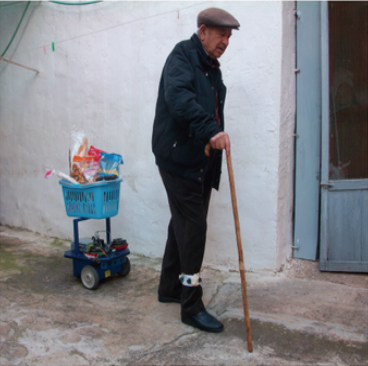
\includegraphics[width=0.4\textwidth]{figs/img/CompaRob}
   \caption{CompaRob Robot}
   \label{fig:CompaRob}
\end{figure}

\begin{figure}[b]
   \centering
   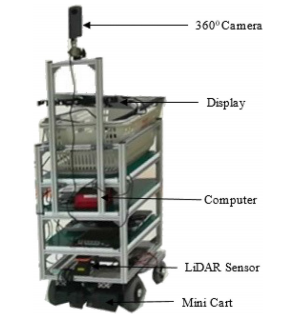
\includegraphics[width=0.38\textwidth]{figs/img/ShoppingSuportRobot}
   \caption{Shopping Support Robot}
   \label{fig:ShoppingSup}
\end{figure}

\begin{figure}[b]
   \centering
   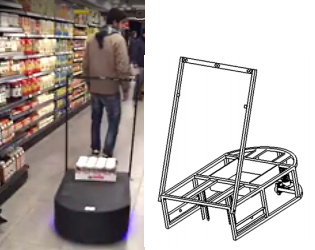
\includegraphics[width=0.45\textwidth]{figs/img/SmartCart}
   \caption{Smart Cart Robot}
   \label{fig:SmartCart}
\end{figure}

\vspace*{12pt}
\noindent
In the current project, we are implementing XBee S2C RF radios, which are inexpensive and easily configurable, as a remote target device that is carried by the user. The robot will be able to track this remote instead of using line of sight methods~\cite{Miah2018-Intelligent}. In addition to the XBee S2C RF radios, we will equip the robot with a parabolic reflector, which improves radio reception at various distances and angles, \textit{i.e.,} angle of arrivals of RF signals from the remote, based on research done previously in this type of robot localization and mapping~\cite{Miah2018-Intelligent}~\cite{Li2013ANA}.

\vspace*{12pt}
\noindent
The approach using signal strength of RF signals also requires an understanding of multipath interference which is common in RF based wireless positioning sensing systems. Authors in~\cite{xie_jiang_zhao_zhang_2019} explain that using course estimation calculations such as received signal strength indicator (RSSI) and time difference of arrival (TDoA) is key to compensate for the multipath interference in received signals.

\vspace*{12pt}
\noindent
The work in ~\cite{ladd_bekris_rudys_kavraki_wallach_2005} shows a different approach to the multipath issue by using an IEEE 802.11b wireless ethernet device to measure RF signals. This device system was used because it is communicable between a mobile device and a localization based service with low complexity for the user.

\vspace*{12pt}
\noindent
Also, in~\cite{lindhe_johansson_bicchi_2007}, the research states several other ways to counteract the multipath fading with methods such as antenna diversity, frequency spreading, or adaptive antenna arrays. The method used in this paper was to sample the radio signal strength (RSS) at discrete points without too much deviation from the robot's desired position in an indoor environment.

\vspace*{12pt}
\noindent
Lastly, in~\cite{Lindhe2009} the method that is utilized exploits multipath fading by measuring the signal-to-noise ratio (SNR) and adjusting the robot's motion to spend more time where the channel strength is greater.

\vspace*{12pt}
\noindent
All of the solutions that were found required line-of-sight communication between the robot and the user. In this project we aim to use the XBee S2C RF radios and a parabolic reflector combined into a rotating system similar to the one presented in~\cite{Miah2018-Intelligent} in order to have the robot track the customer through a store without using line-of-sight sensing. The major challenge of this implementation will be estimating the distance between the robot and the remote in varying environments.

%----------------------------------------------------------------------
\section{Report Organization}
%----------------------------------------------------------------------
\begin{itemize}
    \item Chapter \ref{ch: Chapter1} discusses the background and goals of the project and what other similar projects have accomplished.
    \item Chapter \ref{ch: Chapter2} explains how the robotic cart system in this project is broken down fundamentally, and the components used to build the robot.
    \item Chapter \ref{ch: Chapter3} goes over the design of the parabolic reflector arrays and how they were set up on the robot.
    \item Chapter \ref{ch: Chapter4} provides an explanation of the algorithms that were used to create the code to make the robot move.
    \item Chapter \ref{ch: Chapter5} discusses the implementation of all the parts onto the robot and the experimental results obtained when running the robot.
    \item Chapter \ref{ch: Chapter6} concludes the project work and discusses future endeavors on this project.
\end{itemize}

%%% Local Variables:
%%% mode: latex
%%% TeX-master: "../finalReport"
%%% End:

%======================================================================
\chapter{System Architecture}
\label{ch: Chapter2}
%======================================================================

%----------------------------------------------------------------------
\section{System Block Diagram}
%----------------------------------------------------------------------
The overall system architecture of this project consists of two subsystems which
are the Mobile Cart and the Remote Target, which is held by the user or
customer, as shown in Fig. \ref{fig:sys_block_diag}. The proposed smart robotic
cart is a wheeled robot that sends and receives radio signals to follow the
remote target which acts as the beacon for the robotic cart system.

\vspace*{12pt}
\noindent
The high-level system block diagram of the proposed robotic cart (prototype) is shown in Fig. \ref{fig:sys_block_diag}. There are three inputs to the proposed cart system. The robotic cart is supplied with power through a battery that is mounted in the chassis of the robotic cart. There will be an on/off switch to allow the system to be powered down when not in use. This will save the battery from being drained by the XBees in the reflector array. The motion of the robotic cart is dependent on the motion of the remote.

\begin{figure}[H]
  \centering
  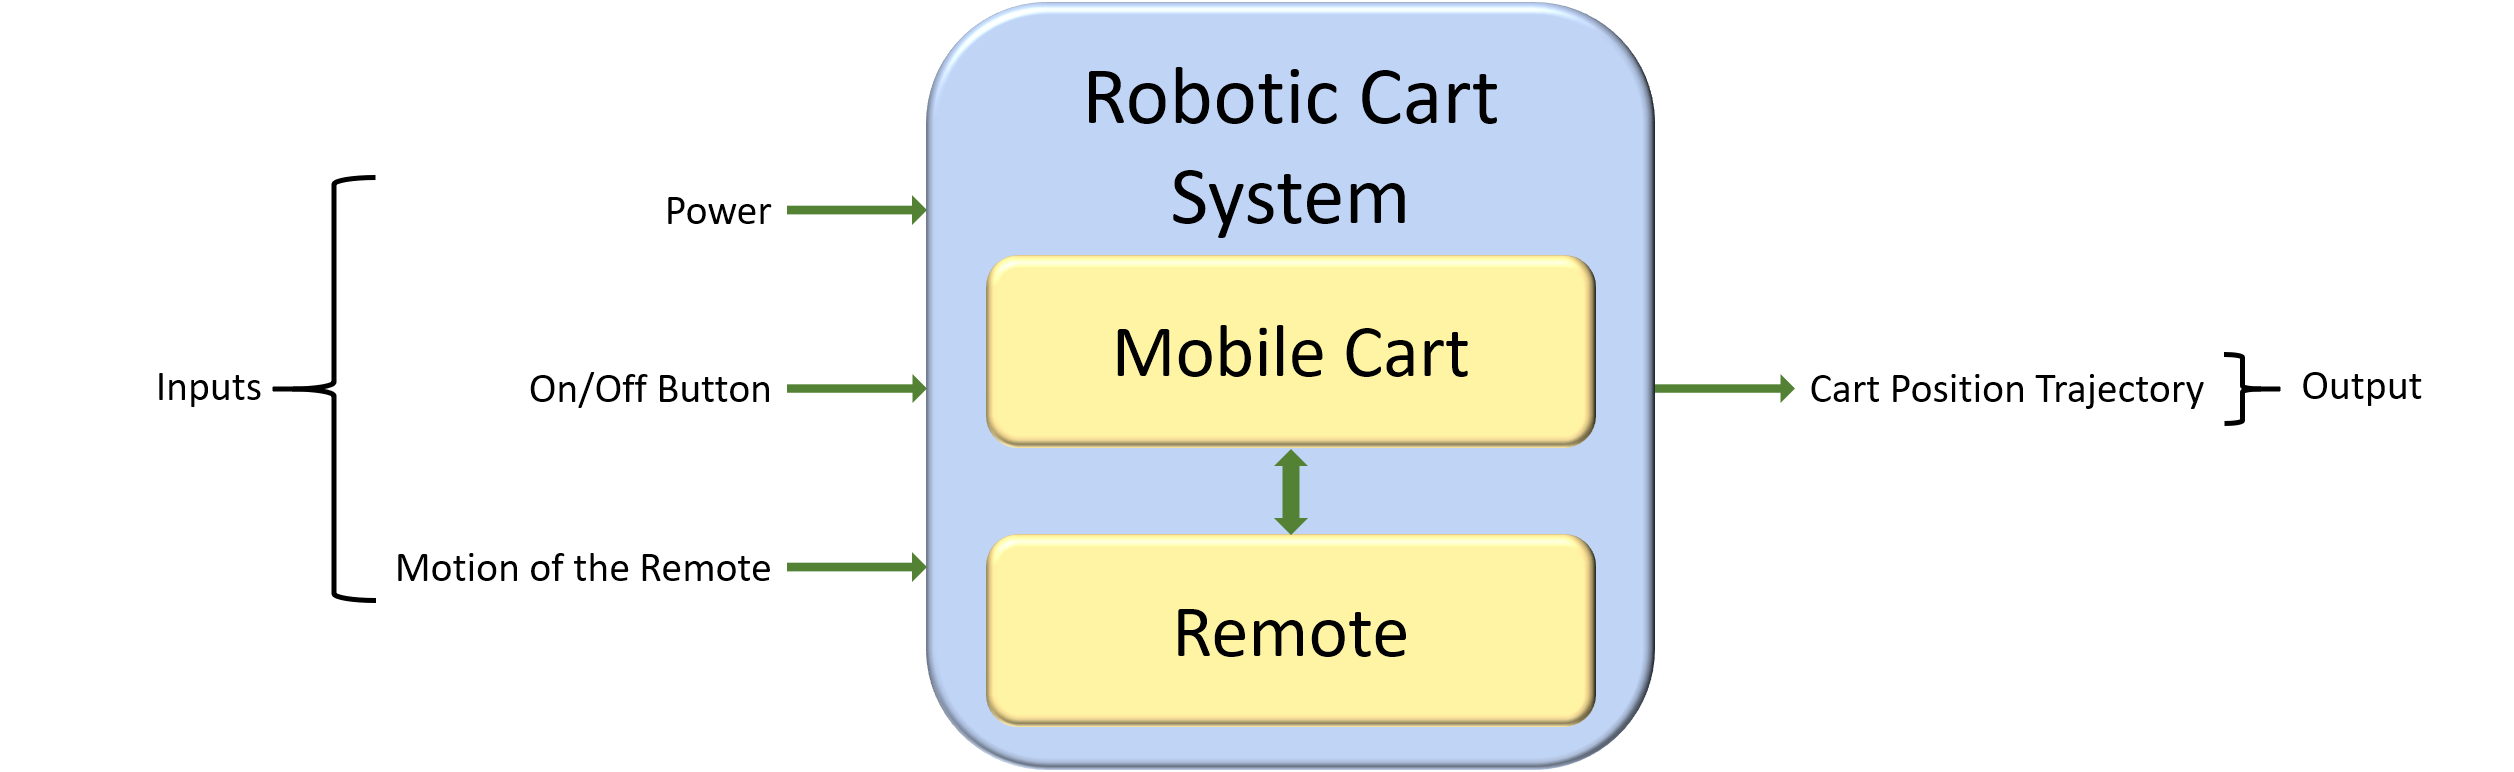
\includegraphics[width=\textwidth]{figs/img/systemBlockDiagram.png}
  \caption{System level block diagram detailing inputs and outputs to the
    robotic cart system.}
	\label{fig:sys_block_diag}
\end{figure}

\vspace*{12pt}
\noindent
The main output of the system is the position trajectory of the robotic cart in its environment. When the user moves with the remote target, the robotic cart is designed to follow the user.



%----------------------------------------------------------------------
\section{Subsystem Block Diagrams}
%----------------------------------------------------------------------
The Mobile Cart and the Remote Target subsystems are two separate operations
within the robotic cart system that run simultaneously. The two subsystems
communicate with one another by relaying radio messages between them. The first
block diagram is of the Remote Target subsystem shown in Fig.
\ref{fig:remote_block_diag}. Of the two subsystems the Remote Target is the
simplest since it only requires an XBee module attached to a 7.4V Li-Po battery
with a voltage regulation circuit since the XBee has a smaller input voltage of
3.3 volts. The two inputs for this system are the battery power and the incoming
RF messages which are passed through the RF transceiver Module and output the
outgoing RF messages.

\begin{figure}[H]
  \centering
  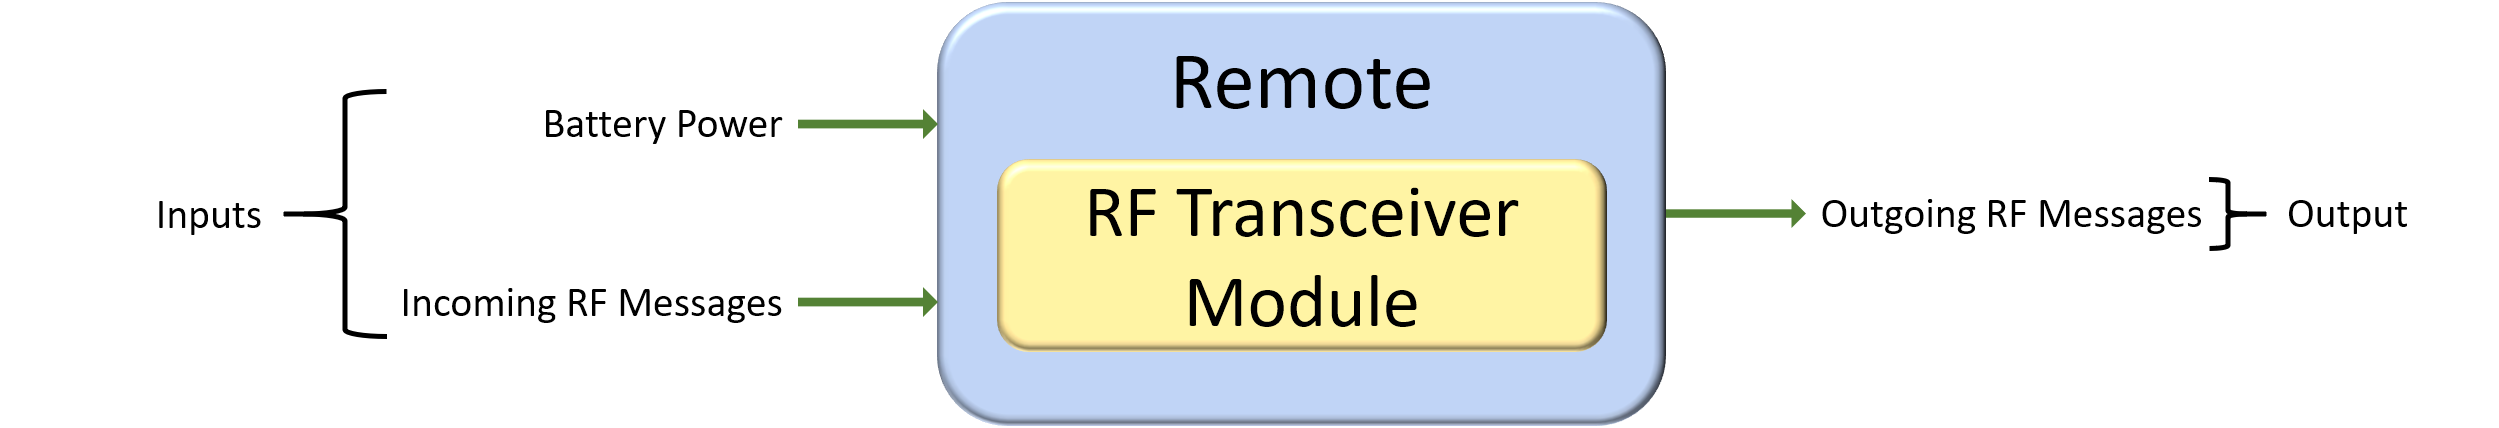
\includegraphics[width=\textwidth]{figs/img/remoteBlockDiagram.png}
  \caption{Remote Target block diagram}
  \label{fig:remote_block_diag}
\end{figure}

\vspace*{12pt}
\noindent
The Mobile Cart subsystem block diagram, shown in Fig.
\ref{fig:mobile_block_diag}, is the most complex of the two subsystems.The cart requires a power source, which will be a 7.4V, 8,000 mAh Li-Po battery since the
Li-Po works well with powering the embedded computer (BeagleBone Blue). The
power to the subsystem will be toggled by an on/off switch located on the
chassis of the robotic cart. The final input to the mobile cart subsystem is the
incoming RF signals. These incoming RF signals are passed to the direction
sensitive RF receivers which output the signals to the dual-direction
multiplexer. The dual-direction multiplexer then takes the four inputs from the
direction sensitive RF receivers and passes one output into the embedded
computer. Once the embedded computer gets these signals it can calculate the
localization and navigation algorithms and pass the information to the DC
motors.

\begin{figure}[H]
  \centering
  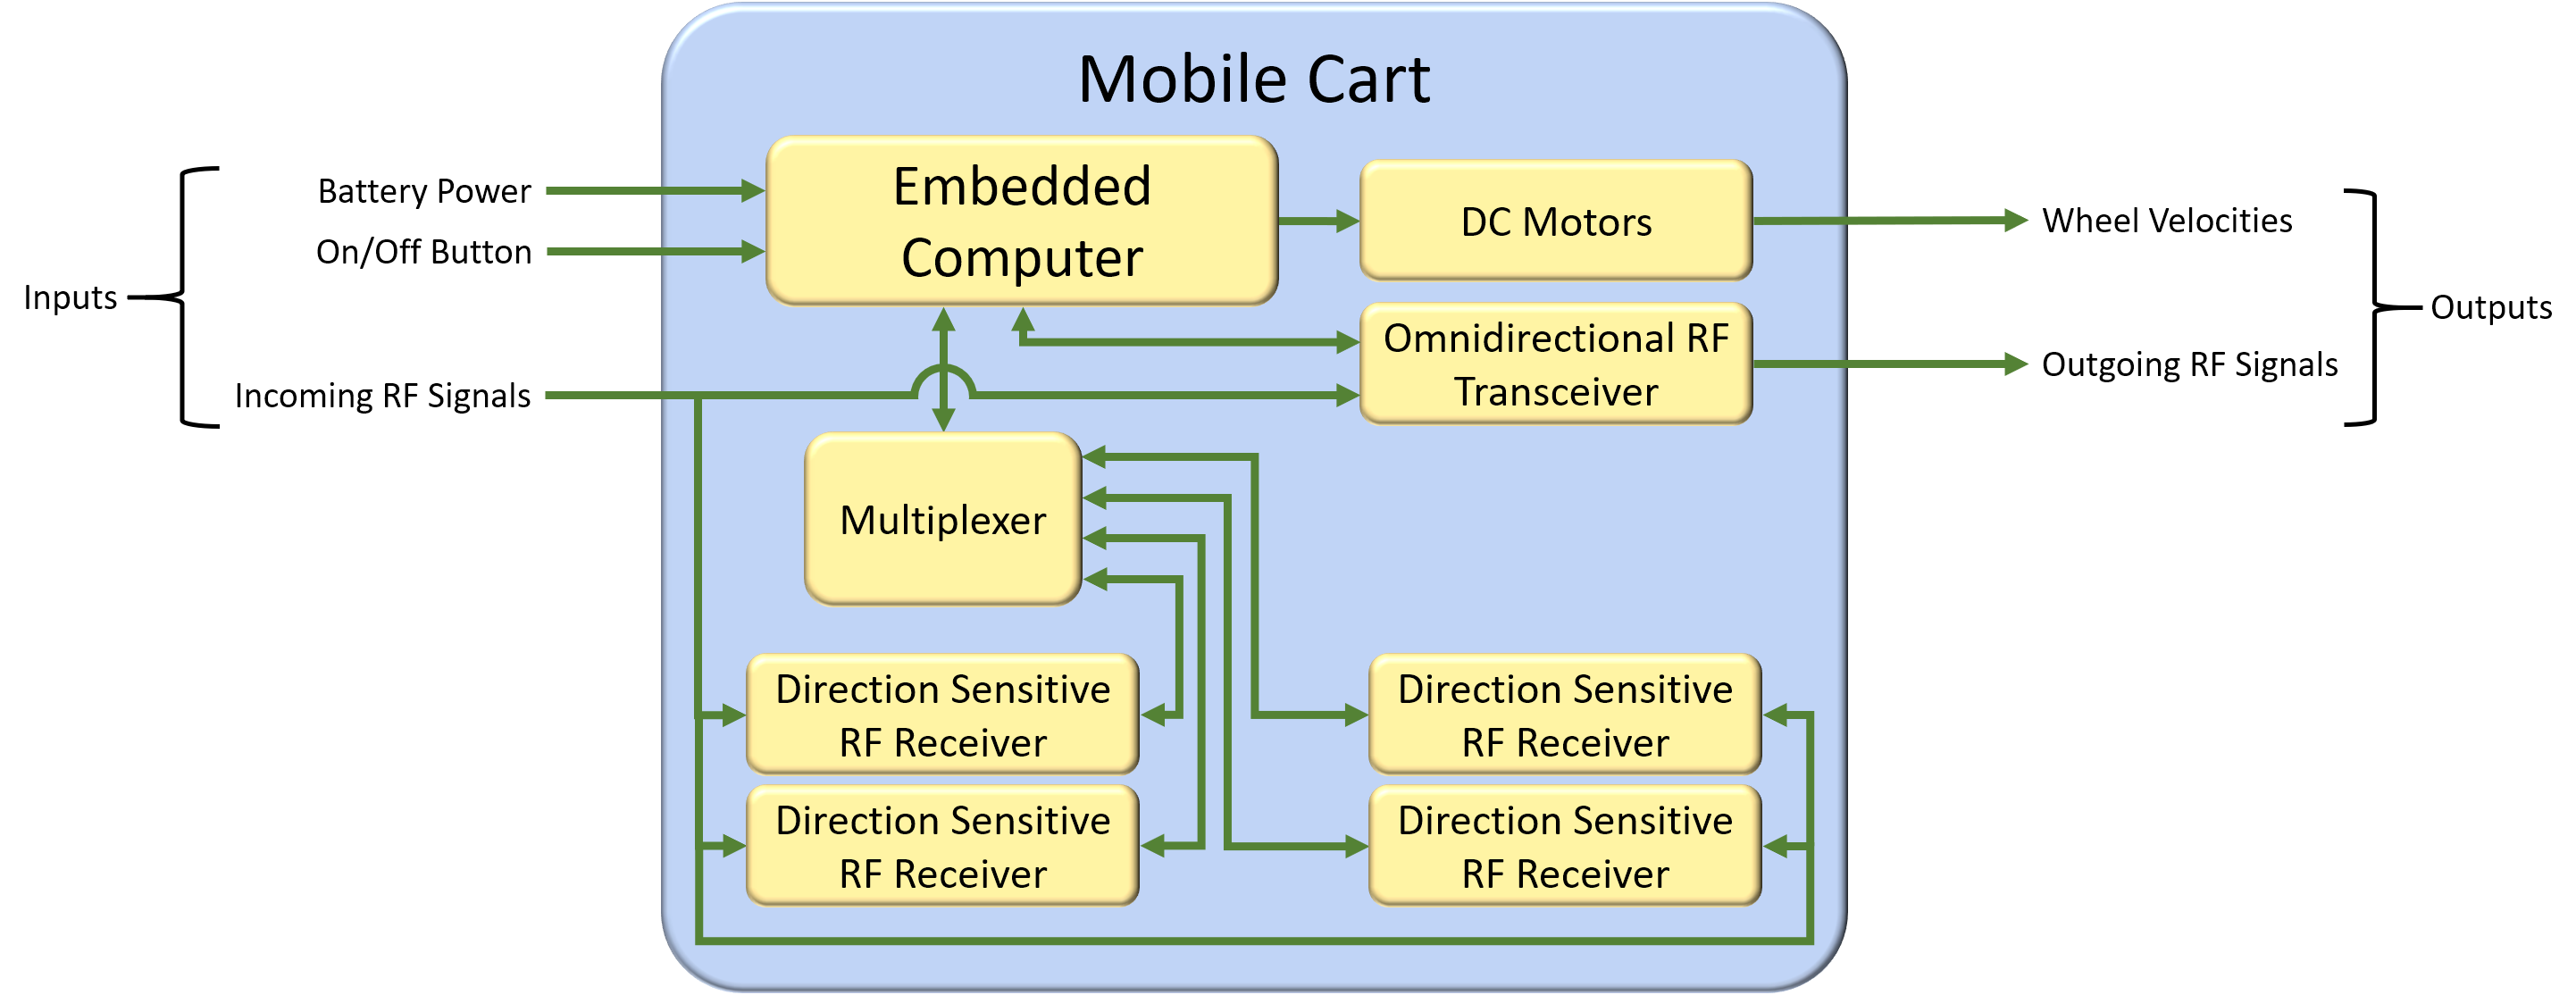
\includegraphics[width=\textwidth]{figs/img/mobileCartBlockDiagram.png}
  \caption{Block diagram showing the subsystem-level components of the proposed robotic cart.}
  \label{fig:mobile_block_diag}
\end{figure}

\vspace*{12pt}
\noindent
There are two outputs of the mobile cart subsystem. The first is the wheel velocities that move the cart and are passed from the DC motors. Lastly, the incoming RF signals are passed to our omnidirectional RF transceiver which outputs the outgoing RF signals.


%----------------------------------------------------------------------
\section{System Components}
\label{sec:System Components}
%----------------------------------------------------------------------

There are several components that are required for the mobile cart system.
Although some of these parts are available in the Bradley University laboratory,
other parts must be purchased. The parts that exist in the lab are listed in
\autoref{tab:Partslablist}. Also, \autoref{tab:Partslist} shows the list of
parts that were purchased. The parts compiled in the lists are the required
parts needed to build two smart robotic cart systems.

\begin{table}[h!]
  \centering
  \caption{Parts Available in Laboratory}
  \begin{tabular}{c|c}
      \toprule
      \textbf{Quantity} & \textbf{Parts}\\
      \toprule
      2 & Budget Bot Chassis\\
      4 & 10 uF Ceramic Capacitor\\
      4 & LM1117 Regulator\\
      8 & 9V Batteries\\
      4 & Solderable PCB Boards\\
      3 & XBee USB Adapter\\
      \bottomrule
      %\multicolumn{2}{r|}{\textbf{Total}} & \$ 562.34\\
      %\bottomrule
  \end{tabular}
  %\caption{Parts Available in Laboratory}
  \label{tab:Partslablist}
\end{table}

\begin{table}[h!]
  \centering
  \caption{Purchased parts for the Robotic Cart Project}
  \begin{tabular}{c|c|c}
    \toprule
    \textbf{Quantity} & \textbf{Parts} & \textbf{Price}\\
    \toprule
    4 & Pololu 37D Metal Gear motor 4751 & \$ 39.95\\
    12 & XBee S2C Module & \$ 23.10\\
    10 & XBee Adapter Board & \$ 4.99\\
    2 & Twotrees 4 Lead Nema 17 Stepper Motor & \$ 9.99\\
    1 & 4-Pin JST SH Connector - 20 Pack & \$ 7.99\\
    1 & 6-Pin JST SH Connector - 10 Pack & \$ 9.99\\
    1 & Aluminum Foil Tape - 2 in x 5 yd & \$ 6.05\\
    2 & Ovonic 7.4V 8000mAh LiPo Battery & \$ 40.99\\
    4 & Multiplexers & \$ 15.99\\
    \bottomrule
    \multicolumn{2}{r|}{\textbf{Total}} & \$ 562.34\\
    \bottomrule
  \end{tabular}
  %\caption{Purchased parts for the Robotic Cart Project}
  \label{tab:Partslist}
\end{table}

\vspace*{6pt}
\noindent
The main components for this project are the Budget Bot Chassis (Fig.
\ref{fig:budgetBotChassis}), the BeagleBone Blue embedded computer (Fig.
\ref{fig:beagleboneBlue}), and the XBee S2C Modules (Fig. \ref{fig:XBeeModule}).
Another major component is the reflector array that will be used to
directionally receive the RF signals from the remote target that is with the
user.

\begin{figure}
  \centering
  \begin{subfigure}[t]{0.32\linewidth}
    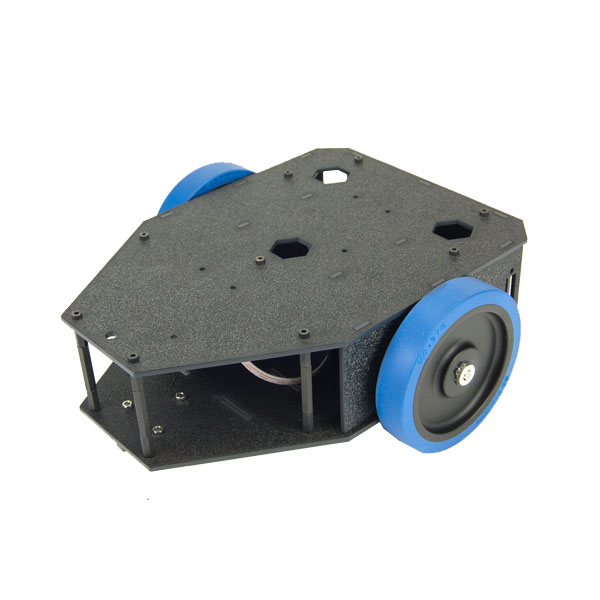
\includegraphics[width=1\linewidth]{figs/img/budgetbot_chassis}
    \captionsetup{width=\linewidth}
    \caption{Budget Bot Chassis}
    \label{fig:budgetBotChassis}
  \end{subfigure}
  \begin{subfigure}[t]{0.32\linewidth}
    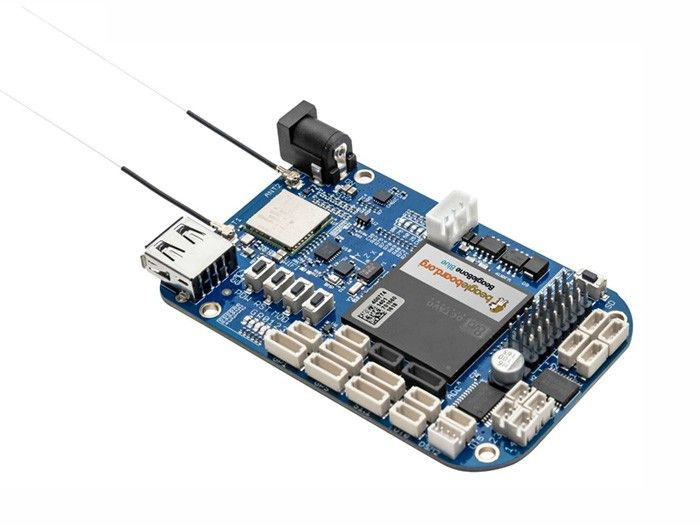
\includegraphics[width=1\linewidth]{figs/img/beaglebone_blue}
    \captionsetup{width=\linewidth}
    \caption{BeagleBone Blue}
    \label{fig:beagleboneBlue}
  \end{subfigure}
  \begin{subfigure}[t]{0.32\linewidth}
    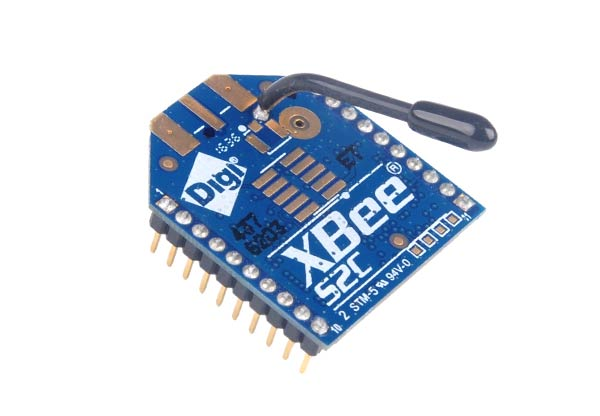
\includegraphics[width=1\linewidth]{figs/img/Xbee-S2C-Module}
    \captionsetup{width=\linewidth}
    \caption{XBee S2C Module}
    \label{fig:XBeeModule}
  \end{subfigure}
\end{figure}

\vspace*{12pt}
\noindent
The reflector array will be mounted on top of the cart with a stepper motor.
There are two reflector designs that were evaluated in this project. The first,
shown in Fig. \ref{fig:parabolodialReflector}, is a paraboloidal reflector which
maximizes the signal strength of the signals that come into the reflector
perpendicularly. Since the remote will be carried by the user, it is likely that
it will be positioned at a higher altitude than the reflector array. The
paraboloidal reflector design may not be able to pick up the signals from the
remote as well because of this. %
%
%
\begin{figure}
  \centering
  \begin{subfigure}[t]{0.5\linewidth}
    \centering
    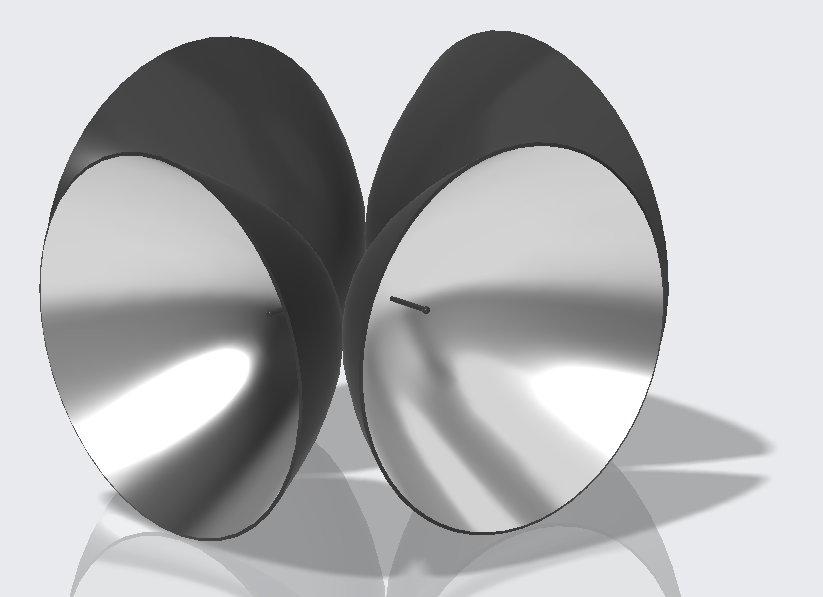
\includegraphics[height=2in\linewidth]{figs/img/paraboloidalReflector}
    \captionsetup{width=\linewidth, justification=raggedright}
    \caption{Paraboloidal Reflector Model}
    \label{fig:parabolodialReflector}
  \end{subfigure}
  \begin{subfigure}[t]{0.4\linewidth}
    \centering
    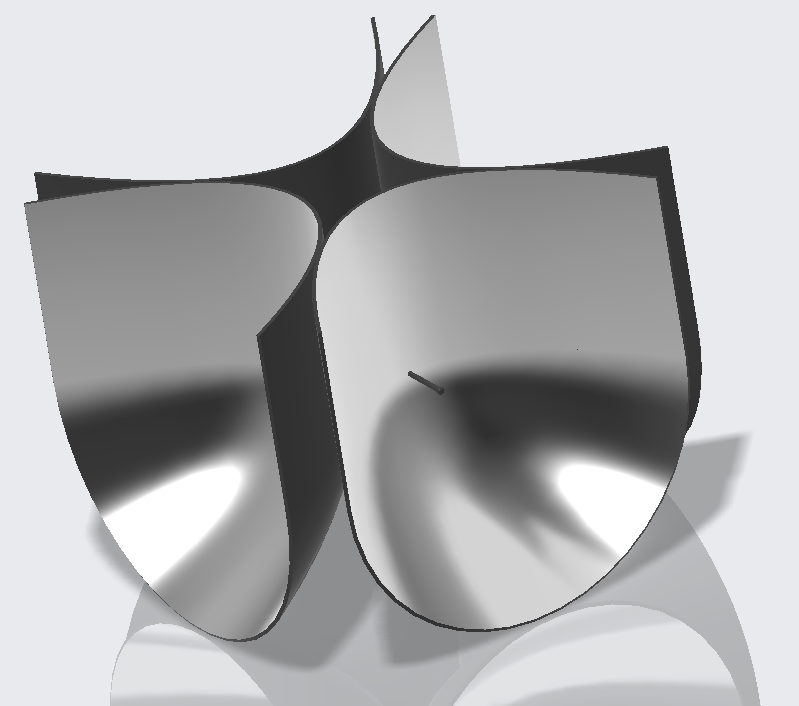
\includegraphics[height=2in\linewidth]{figs/img/parabolicReflector}
    \captionsetup{width=\linewidth, justification=raggedright}
    \caption{Combined Parabolic/Paraboloidal Reflector}
    \label{fig:parabolicReflector1}
  \end{subfigure}
\end{figure}
%
To solve this problem, a combination parabolic/paraboloidal reflector was
designed, as shown in Fig. \ref{fig:parabolicReflector1}. The lower half of this
reflector is paraboloidal in shape to limit the signals coming from below. The
upper part of the reflector is strictly parabolic. This shape focuses the
signals in the horizontal plane, but allows signals from above to still be
received. The plan is to construct both of these reflector designs by 3D
printing the frames, then lining them with reflective foil tape. Both models
will then be tested to determine which design works better.


%----------------------------------------------------------------------
\section{Operation of Robotic Cart System}
\label{sec:Operation of Robotic Cart System}
%----------------------------------------------------------------------
The mobile cart was controlled by a central embedded computer which is the BeagleBone Blue since it is ideal in robotics control. Two DC motors were used to drive wheels and move the cart. Five XBee modules on the cart were used to allow communication with the remote target. One of these radio sensors was mounted on top of the cart to broadcast in all directions. The other four sensors were placed inside parabolic reflectors at right angles to each other. This sensor array was mounted on a stepper motor to allow rotation.


%%% Local Variables:
%%% mode: latex
%%% TeX-master: "../finalReport"
%%% End:

%======================================================================
\chapter{Implementation}
\label{ch: implementation}
%======================================================================

For the implementation of this project we had to start from scratch since this was a new project concept introduced by our advisor Dr. Miah. There have been senior projects in the past that have used XBees to get signal strength but there is very little overlap between these projects to substantiate where our project needed to start from. For this project we had to first build a mobile robot and a remote to use for testing. We then had to build a code base to control the mobile robot that was then implemented with our test algorithms.

%----------------------------------------------------------------------
\section{Robot Assembly}
\label{sec:Robot Assembly}
%----------------------------------------------------------------------

For this project we needed a Remote Target and Smart Robotic Cart that we designed and implemented from off the shelf components.  As mentioned above in section \ref{sec:System Components}, some of our components came from what the school already owned as well as some we had to buy specifically for this project listed in \autoref{tab:Partslablist} and \autoref{tab:Partslist}.

\vspace*{12pt}
\noindent
Since the school already owned the Budget Bot chassis, we decided to build our Smart Robotic Cart with them. The Budget Bot chassis needed to be modified slightly to work with our project. The main change we made was swapping out the motors that came with the Budget Bot for Pololu 27D Metal Gear motors since the original motors have a max speed of 212 RPM or 1.09m/s and the new motors have a max speed of 530 RPM or 2.72m/s when using the wheels with a diameter of 98mm. By switching out the motors we are able to achieve our goal of matching an average person's walking speed of 1.5m/s. The other modifications to the chassis are a hard power switch to directly cut off power to the XBee modules in the reflector and a power indicator LED to let us know when this switch was on.

\vspace*{12pt}
\noindent
As shown in Fig. \ref{fig:FinalizedRobot}, our next step was to attach the BeagleBone Blue microcomputer, XBee reflector array assembly, and breadboard to the top of the robot. We also installed a 2-cell LiPo battery inside the chassis of the mobile cart that delivers power to the BeagleBone Blue directly and the breadboard through the switch.

\begin{figure}[H]
    \centering
    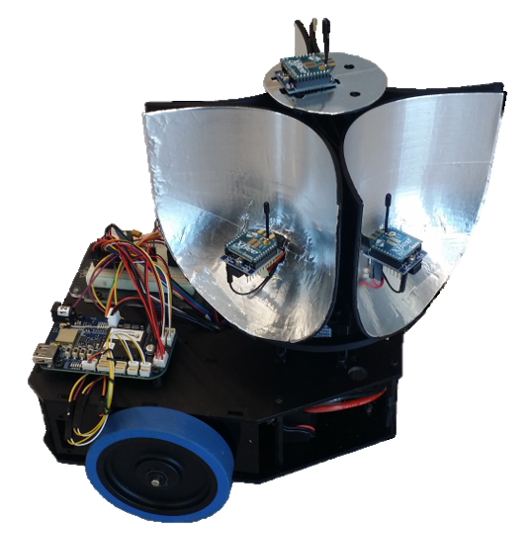
\includegraphics[width=0.5\textwidth]{figs/img/Finalized_robot.png}
    \caption{Overall Prototype of the Robotic Cart}
    \label{fig:FinalizedRobot}
\end{figure}

The power supplied to the breadboard is sent through a regulator circuit to drop it down from the 7.4V of the LiPo to 3.3V of the XBee. This circuit is also used on the remote which consists of a 7.4V LiPo battery and the XBee module with voltage regulator in between. This voltage regulator is built out of a LM117 regulator and a 10uF ceramic capacitor between the input and output pins of the regulator as shown in Fig. \ref{fig:PowerConverter}.

\begin{figure}[H]
    \centering
    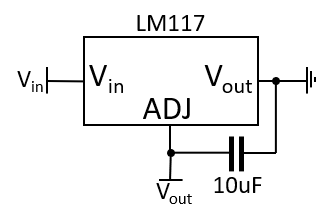
\includegraphics[width=0.5\textwidth]{figs/img/PowerConverter.png}
    \caption{Final Version of the Robotic Cart}
    \label{fig:PowerConverter}
\end{figure}

\vspace*{12pt}
\noindent
The reflector array assembly from \autoref{sec:customReflector} was mounted on a stepper motor that was then attached to the robot chassis using a 3D printed bracket. This bracket was then attached to the chassis using bolts. Another feature of this bracket is that it had a stop block built into the top of it to automatically zero the reflector array when the robot starts up.

\vspace*{12pt}
\noindent
The Xbee modules from the reflector array posed a bit of a problem when it came to connecting them to the BeagleBone Blue. The BeagleBone Blue has five UART ports if one were the three standard UART ports and tow others found in the USB and UART-GPS. Unfortunately though this does not work since UART port zero is tied to the council used to communicate with it from a computer. Since this port is reserved for this function that reduces the number of usable ports down to four and we need to have five XBees in these ports. Our solution to this was to use two of the GPIO pins, two of the UART ports, and a two-way multiplexer. With this setup we can directly connect one of the UARTs to the top XBee and then rout the other four side XBee modules through the MUX so only one UART port is needed for them.


%----------------------------------------------------------------------
\section{Code Base}
\label{sec:Code Base}
%----------------------------------------------------------------------

For the project we needed some base functionality to use with the main follower program so it can interact with the other components in the system. The BeagleBone Blue already has a set of ports on it that we can access and control using the Robot Control Library from Strawson Design ~\cite{Robot_Control_Library}.

\vspace*{12pt}
\noindent
For the project we also built some custom libraries on top of the Robot Control Library to handle XBee Frames, AT Commands, and the stepper motor. The XBee Frames library takes a given block of data containing our message and then packages it into a XBee Frame to send over UART to the XBee module we want to interact with. The XBee communications library also handles received messages from the XBee module and validates the received frames integrity and extracts the message data from it. On top of the XBee communications library we also have a library that generates AT Commands to package in the XBee Frames. The AT Command library also handles extracting response data from the AT Response Command structure and validates it.

\begin{figure}[H]
  \centering
  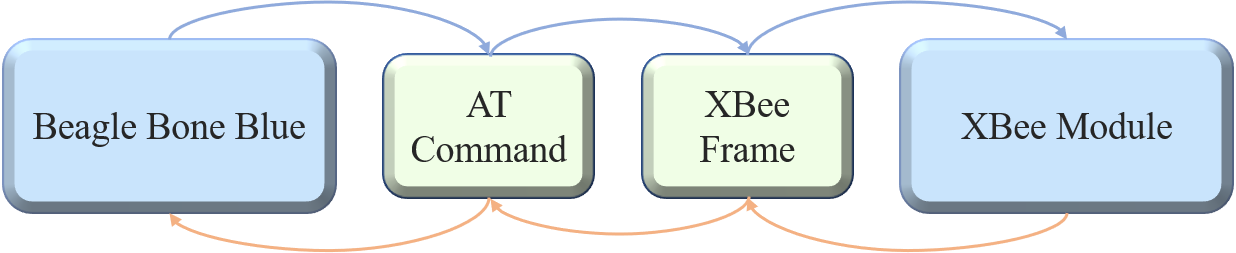
\includegraphics[width=\textwidth]{figs/img/Command Process Diagram.png}
  \caption{Process for XBee Communication over UART}
  \label{fig:CommandProcessDiagram}
\end{figure}

\vspace*{12pt}
\noindent
The final custom library is the stepper motor control library. This library had to be written ourselves since instead of using a dedicated stepper motor controller for our project we were using two of the regular DC motor control ports that are build into the BeagleBone Blue. The library handled translating how many steps to turn into the phase states to be sent to the DC motor ports that are connected to the stepper motor. The library also helped to keep track of basic information related to the stepper motor such as what its current angle should be.

%----------------------------------------------------------------------
\section{Experimental Results}
\label{sec:Experimental Results}
%----------------------------------------------------------------------

In this project after we had the Robotic Cart, Remote Target, and a code base to handle the specifics we started testing different variants of our algorithm explained in \autoref{sec:locAndNavAlgos}. There were two main types of variants we put together, one type the stepper motor is locked preventing the reflector from turning and in the other we use the stepper motor to sweep through a set of angles.

\subsection{Rotating Reflector Tests}

The first type of test we ran was where the robot would zero out the arrays rotation with the stepper motor then move in nine degree increments taking measurements as it went. A sweep ends when the motor has turned 81 degrees since at that point, with the four sides of the reflector, a full 360 degrees has bean scanned.

\vspace*{12pt}
\noindent
This method offers us a sufficiently dense set of data to base our angle predictions off of but at the cost of having to wait until a entire sweep of the reflectors is completed. With this data we first put together a simple test that would continuously be sweeping and moving at the same time. Though this version did successfully follow the remote it had some errors in the robot's navigation trajectory. For example, the robot would correctly turn towards the remote, however, if it picked up a stronger signal from the XBee reverberations, it would drive off in a different direction. The robot would eventually find its way back into alignment and resume moving towards the remote.

\vspace*{12pt}
\noindent
The next version that used a rotating reflector, as well as the final version, works mostly the same as the first version but with some improvements to its navigation. The first big fix is that we determined that the oscillation we were seeing in the first test were a result of turning while also rotating the reflector which would add additional rotation to the measurements in global scope. Due to how our robot is designed we can only rotate the reflector array 90 degrees but to properly fix this rotation issue we would need to rotate the reflector more or less during a sweep to compensate for the robots rotation. Our compromise was simply to allow the robot to always move forward but to alternate between getting measurements and then rotating the robot based on the measurements. In this version some additional windowed filters to average out the angle measurements were added, which did help to reduce the effects of random angles from noise in the system. We also applied offsets to each of the directional receivers revived signal strengths based off the data that we had collected while testing it. This offset was needed due to each side having a different minimum that it would cap out at.

\subsection{Locked Reflector Tests}

The locked reflector tests were ran in between our first algorithm and our final algorithm which ultimately used a sweeping function to capture the XBee signals. These algorithms were an attempt to reduce the time needed to get a set of measurements from the reflector by zeroing its rotation and then keeping it locked in the zeroed position. Since the data from this is relatively sparse we tried three different ways to fill in the gaps in the data from only the four cardinal directions. The first of these three methods was to try and select a strongest direction that the signal was coming from and then which of its two neighbor directions had the next strongest signal. With these two strengths the algorithm would then try to interpolate between these two angles based on the difference of the strengths between them. This method could work but due to the time constraints of our project, we did not have enough time to implement and test this method.

\vspace*{12pt}
\noindent
The other two methods that we tried with the locked reflector were both different variants on machine learning algorithms based on a small pool of data we had collected. The first algorithm tested was K Nearest Neighbors then followed up by a Neural Network for our final fixed rotation test. Both of these algorithms failed to produce any meaningful results due to the fact that we had a very small pool of data to work off of compared to the large amounts of data needed to perform machine learning algorithms. These algorithms, with the small data pool size, did not perform well with the noise in the signals.

\subsection{System noise}

In both our fixed and sweeping experiments a underlying issue is the amount of noise our system produces. The first type of noise that occurs is noise from the Multipath Effect where the signals bounce off of obstacles around it adding constructing and destructive interference randomly based off of the robots surroundings. The second noise was from internal noise in the XBees which was worse that we had expected. We managed to isolate the XBee internal noise by using an anechoic chamber where we did see all the signals strengths become stronger but the base noise from the XBees persisted. The noise coming from the XBees tends to be about 2 to 6 dBm on average. The change from facing towards the remote then away from the remote is about 13 to 15 dBm. These ranges result in the occasional measurement that flip flops which reflector is actually facing the remote. The noise can be seen in our test measurements we collected where we, at set rotations, record a burst of 300 measurements as seen in Fig. \ref{fig:SensorDataGraphs}

\begin{figure}[H]
    \centering
    \begin{subfigure}{0.50\textwidth}
        \centering
        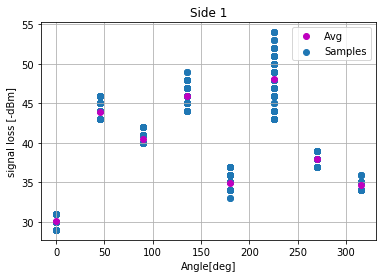
\includegraphics[width=0.95\textwidth]{figs/img/Side1_Data.png}
        \label{fig:Side1Dat}
    \end{subfigure}%
    \begin{subfigure}{0.50\textwidth}
        \centering
        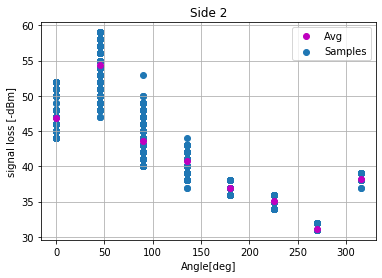
\includegraphics[width=0.95\textwidth]{figs/img/Side2_Data.png}
        \label{fig:Side2Dat}
    \end{subfigure}
        \begin{subfigure}{0.50\textwidth}
        \centering
        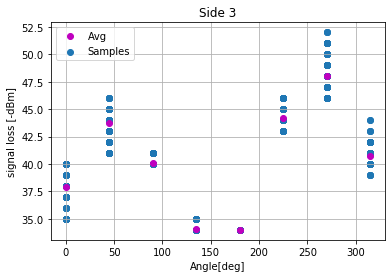
\includegraphics[width=0.95\textwidth]{figs/img/Side3_Data.png}
        \label{fig:Side3Dat}
    \end{subfigure}%
    \begin{subfigure}{0.50\textwidth}
        \centering
        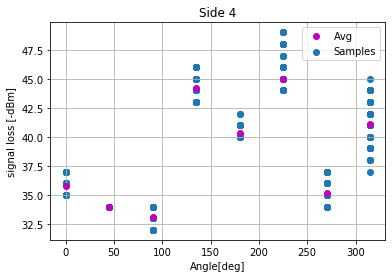
\includegraphics[width=0.95\textwidth]{figs/img/Side4_Data.png}
        \label{fig:Side4Dat}
    \end{subfigure}
    \caption{Navigation Algorithm Details}
    \label{fig:SensorDataGraphs}
\end{figure}

\subsection{Distance}
This project initially planned to use the top XBee modules signal strength to determine the distance to the remote.  In practice, though, it was determined to be practically impossible with our setup.  The free space path loss equation was used as a base equation to work from for implementing this feature in the project.  The issue arises initially from that the free space path loss failed to return a usable distance by itself whenever any form of obstacle ends up in the line of sight path to the remote.  The free space path loss equation also is thrown off by any reflective surfaces around it due to the multipath effect.  These issues could be potentially solved by Simultanius Localization and Mapping algorithms like EKF-SLAM.  Unfortunately, this approach also does not work since it relies on a known global reference point that is absent in this project design. Since within the allotted time for the project, no viable solution was found, it was decided that the distance measurement would be put on hold for future work on the project



\section{Simulation using Robot Simulator}

Before constructing the physical robot prototype, a simulation was performed using a commercial robot simulator CoppeliaSim. However, since RF signal behavior depends highly on the environment, the system could not be fully simulated. This section explains the steps taken to simulate the proposed robotic cart.

\vspace*{12pt}
\noindent
First, a model of the Budget Bot chassis was created in CoppeliaSim. The model is shown in Fig. \ref{fig:budgetBotModel}. The model was designed with the same dimensions as the physical chassis to accurately simulate the robot kinematics. Details on modeling a robot chassis in CoppeliaSim can be found in \autoref{ch: coppSimModeling}. Although \autoref{ch: coppSimModeling} explains the modeling of a robot chassis that is different than the Budget Bot chassis, the concepts are the same for modeling any robot chassis.

\begin{figure}
    \centering
    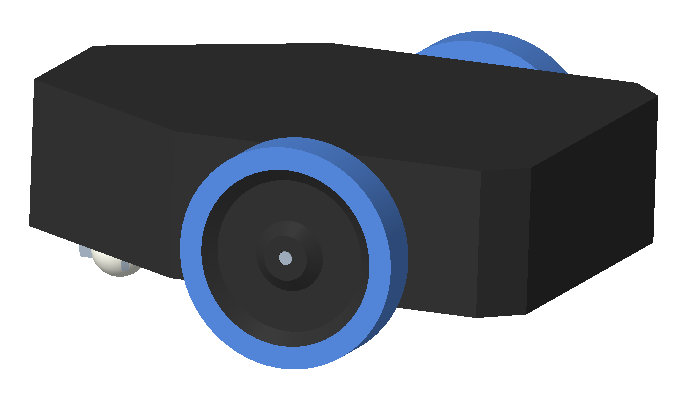
\includegraphics[width=0.6\textwidth]{figs/img/budgetBotModel.png}
    \caption{Model of Budget Bot Chassis}
    \label{fig:budgetBotModel}
\end{figure}

\vspace*{12pt}
\noindent
MATLAB code was written to control the simulation. The actual distance between the robot and the remote was measured, then random noise was added with a mean of 0 and a standard deviation of 0.07. This noisy measurement was then used in the navigation algorithm to determine how to drive the robot (see \autoref{subsec:navAlgo}). An image of the simulation is shown in Fig. \ref{fig:coppSimExample}, where the blue sphere represents the remote, and the green dot represents the target point.
\begin{figure}
    \centering
    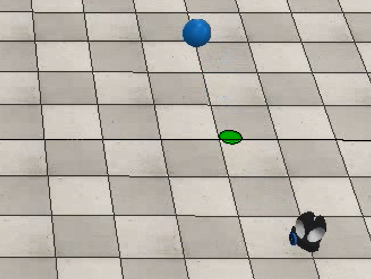
\includegraphics[width=0.5\textwidth]{figs/img/coppSimExample.png}
    \caption{CoppeliaSim Simulation}
    \label{fig:coppSimExample}
\end{figure}


%%% Local Variables:
%%% mode: latex
%%% TeX-master: "../finalReport"
%%% End:

%======================================================================
\chapter{Conclusion and Future Work}
<<<<<<< HEAD:parts/60-conclusion_and_future_work.tex
\label{ch: Chapter6}
=======
\label{ch: conclusionAndFuture}
>>>>>>> 9e3deacdd38258c6493f669a814a6d4aebc5764b:parts/40-conclusion_and_future_work.tex
%======================================================================

%----------------------------------------------------------------------
\section{Conclusion}
%----------------------------------------------------------------------

From what we have seen in this project we would conclude that the robotic cart can indeed successfully follow the remote target radio.


  
\todo[inline]{Complete the conclusion section}

%----------------------------------------------------------------------
\section{Future Work}
%----------------------------------------------------------------------


\todo[inline]{Complete the future work section}

%%% Local Variables:
%%% mode: latex
%%% TeX-master: "../finalReport"
%%% End:


% %----------------------------------------------------------------------
% % APPENDICES
% %---------------------------------------------------------------------- 
\appendix
% % Designate with \appendix declaration which just changes numbering style 
% % from here on
% % Add a title page before the appendices and a line in the Table of Contents
\addcontentsline{toc}{chapter}{APPENDICES} 
% %

%======================================================================
\chapter{Modeling in CoppeliaSim}
\label{ch: coppSimModeling}
%======================================================================

%----------------------------------------------------------------------
\section{Problem Statement}
%----------------------------------------------------------------------
It is important to be able to simulate a robot's behavior before using the
actual robot to help find unexpected behaviors. CoppeliaSim is commercial robot
simulation software with the ability to simulate a robot that would operate in
exactly the way it would happen with a real robot. However, the robot of
interest is not currently included in CoppeliaSim's library that leads to
creating a model of the robot and simulating it before practical implementation.
The following sections explain how to model the Runt Rover robot in CoppeliaSim.

%----------------------------------------------------------------------
\section{Dimensions and 3D Modeling}
%----------------------------------------------------------------------
The Runt Rover robot is geometrically simple, with only a few dimensions being necessary to model the shape of the body and wheels. The dimensions used in this guide are shown in Fig. \ref{fig:runtRoverDims}

\begin{figure}
    \centering
    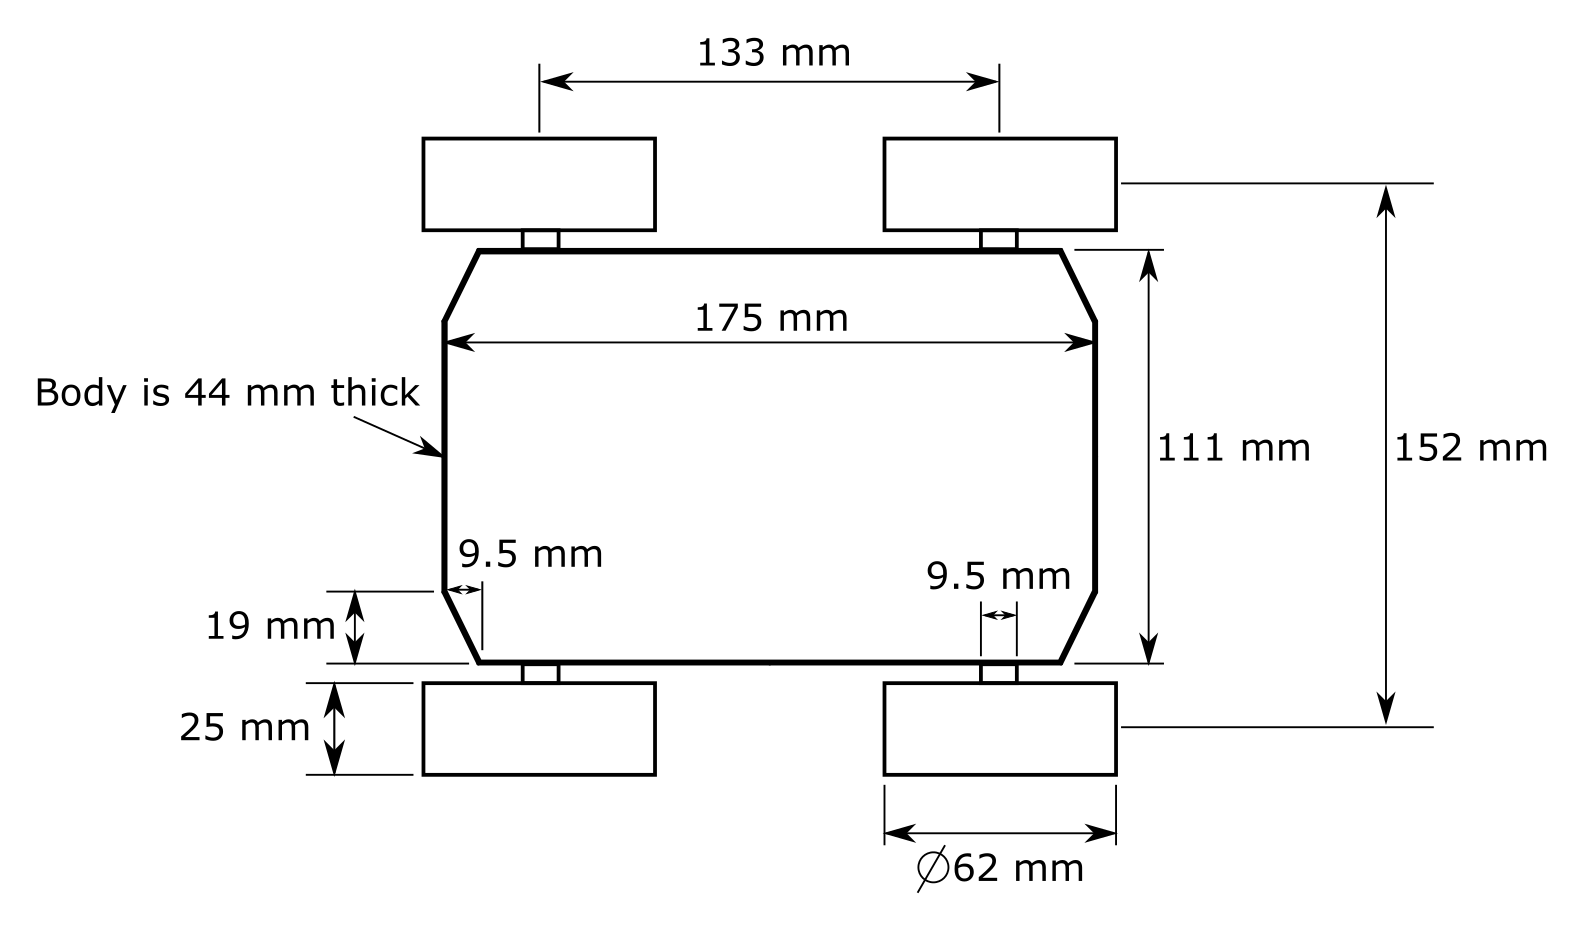
\includegraphics[width=3.5in]{figs/img/runtRoverDimensions}
    \caption{Dimensions of the Runt Rover Robot}
    \label{fig:runtRoverDims}
\end{figure}

The final 3D models are shown in Fig. \ref{fig:runtRoverModels}. An arrow was placed on the body to indicate orientation during simulation.

\begin{figure}
    \centering
    \begin{subfigure}[b]{0.6\textwidth}
        \centering
        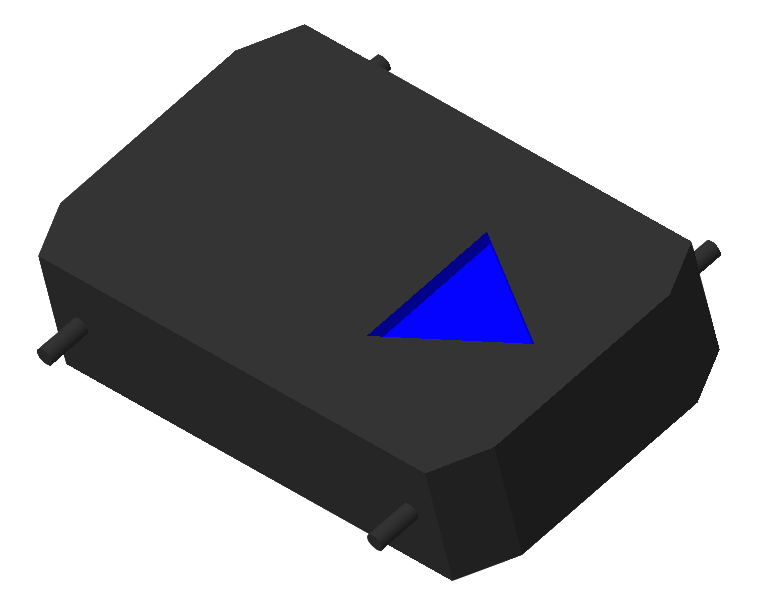
\includegraphics[width=\textwidth]{figs/img/runtRoverChassis}
        \caption{Chassis}
        \label{fig:runtRoverChassis}
    \end{subfigure}
    \hfill
    \begin{subfigure}[b]{0.3\textwidth}
        \centering
        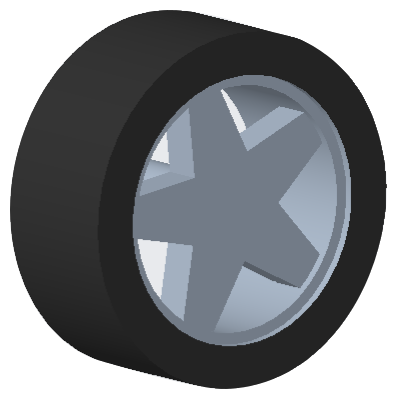
\includegraphics[width=\textwidth]{figs/img/runtRoverWheel}
        \caption{Wheel}
        \label{fig:runtRoverWheel}
    \end{subfigure}
    \caption{Modeled Parts}
    \label{fig:runtRoverModels}
\end{figure}

%----------------------------------------------------------------------
\section{Importing Models}
%----------------------------------------------------------------------
The next step is to import the 3D models into CoppeliaSim. This is accomplished using File \textgreater \ Import \textgreater \ Mesh. If the models were dimensioned in millimeters, the scale must be changed to 0.001 since CoppeliaSim uses meters. Since there are multiple colors in the models, there will be multiple shapes in CoppeliaSim. These can be grouped by dragging one shape onto another. Also, the shapes can be renamed. In modeling the Runt Rover, one chassis and four wheels are needed. The wheels must be placed in the correct locations on the axles.

%----------------------------------------------------------------------
\section{Adding Motors}
%----------------------------------------------------------------------
The robot can be given motors by means of revolute joints. These can be added using Add \textgreater \ Joint \textgreater \ Revolute. For the Runt Rover, one revolute joint was placed at each wheel. The joints should be named according to the wheel location since their names are used to interface the robot with Matlab. These joints are then made invisible by moving them to visibility layer 10. This is achieved in the Object Common Properties dialog box. The joints can be viewed by turning on visibility for layer 10 using the Layers dialog box. In the Object Properties dialog box, there is a button to open the Dynamic Properties dialog box. In this box, make sure the ``Motor enabled'' checkbox is enabled.

%----------------------------------------------------------------------
\section{Dynamic Shapes}
%----------------------------------------------------------------------
The 3D models do not have any dynamic properties within CoppeliaSim. It is recommended to use primitive shapes for the dynamic properties to reduce computation during simulation. For the Runt Rover, the wheels can be dynamically represented as cylinders, and the chassis can be dynamically represented as a cuboid. To add a primitive cylinder, use Add \textgreater \ Primitive Shape \textgreater \ Cylinder, and specify the size to be the same as a wheel. To add a cuboid, use Add \textgreater \ Primitive Shape \textgreater \ Cuboid, and specify the size to be the same as the chassis. These bodies must now be configured with the appropriate dynamic properties.

In the dynamic properties dialog box, make sure the ``Body is respondable'' checkbox is enabled, and enable the first four checkboxes and disable the last four checkboxes in the local respondable mask. Repeat this process on all of the dynamic shapes, alternating between selecting the first four and selecting the last four checkboxes in the local respondable mask. To give the robot mass and inertia, make sure the ``Body is dynamic'' checkbox is enabled, and click the ``Compute mass and inertia'' button. These dynamic shapes should be named according to the parts they represent (FrontLeftWheelDyn, for example). In the Object Common Properties dialog box, assign the dynamic shapes to visibility layer 9 to make them invisible.

%----------------------------------------------------------------------
\section{Linkage}
%----------------------------------------------------------------------
Now it is time to link everything together into one robot. First assign each graphical shape to its corresponding dynamic shape by dragging and dropping it onto the dynamic shape. Then assign the dynamic shapes for the wheels to the corresponding revolute joints in the same way. Finally, assign the revolute joints to the dynamic chassis. The name of the dynamic chassis is the name that will be used to interface with Matlab, so change it to ``RuntRover.'' Assign this shape to be the model base in the Object Common Properties dialog box. To make the bounding box the correct size, select the revolute joints and enable the ``Ignored by model bounding box'' and the ``Invisible during selection'' checkboxes in the Object Common Properties dialog box. Now enable the ``Select base of model instead'' checkbox for each of the visible objects. This allows us to select the entire robot by clicking on any part.

%----------------------------------------------------------------------
\section{Saving the Model}
%----------------------------------------------------------------------
To save this model, go to File \textgreater \ Save model as \textgreater \ CoppeliaSim model. The default location should be in the CoppeliaSim models directory. Create a new directory to contain your models and save the model within that directory. Your model will now be available in the CoppeliaSim library.


%%% Local Variables:
%%% mode: latex
%%% TeX-master: "../finalReport"
%%% End:

% %======================================================================
\chapter{Assembly Instructions}
\label{ch: assemblyInstructions}
%======================================================================

This appendix explains how to assemble the robot from the individual components. Some useful tools to have on hand during the assembly are a 2.5mm Allen key, a pair of needlenose pliers, a wire stripper, a scissors, and an exacto knife. Follow the steps below to assemble the robot.

\vspace*{18pt}
\noindent
\begin{Large}\textbf{Instructions}\end{Large}

\begin{enumerate}[label = \textbf{Step \arabic*.}]
    \item Get a Budget Bot Chassis (Fig. \ref{fig:assemblyBudgetBot}). For this project, a fuse, power switch, and power indicator LED were added to the Budget Bot Chassis. Install a 2-cell LiPo battery inside the Budget Bot. Route the balance plug and battery output cable up through the center hole on top of the Budget Bot.
    \begin{figure}[H]
        \centering
        \includegraphics[width=3.6in]{figs/img/assembly/01-BudgetBot.png}
        \caption{Modified Budget Bot Chassis}
        \label{fig:assemblyBudgetBot}
    \end{figure}

    \item Install a BeagleBone Blue and a solderless breadboard on the Budget Bot using 6mm M3 screws (Fig. \ref{fig:bbblueInstallation}, red circles). Connect the battery's balance plug to the terminal on the BBBlue, and the power output to the breadboard (Fig. \ref{fig:bbblueInstallation}, green circles). Finally, insert the motor cables into the breadboard (Fig. \ref{fig:bbblueInstallation}, blue circle).
    \begin{figure}[H]
        \centering
        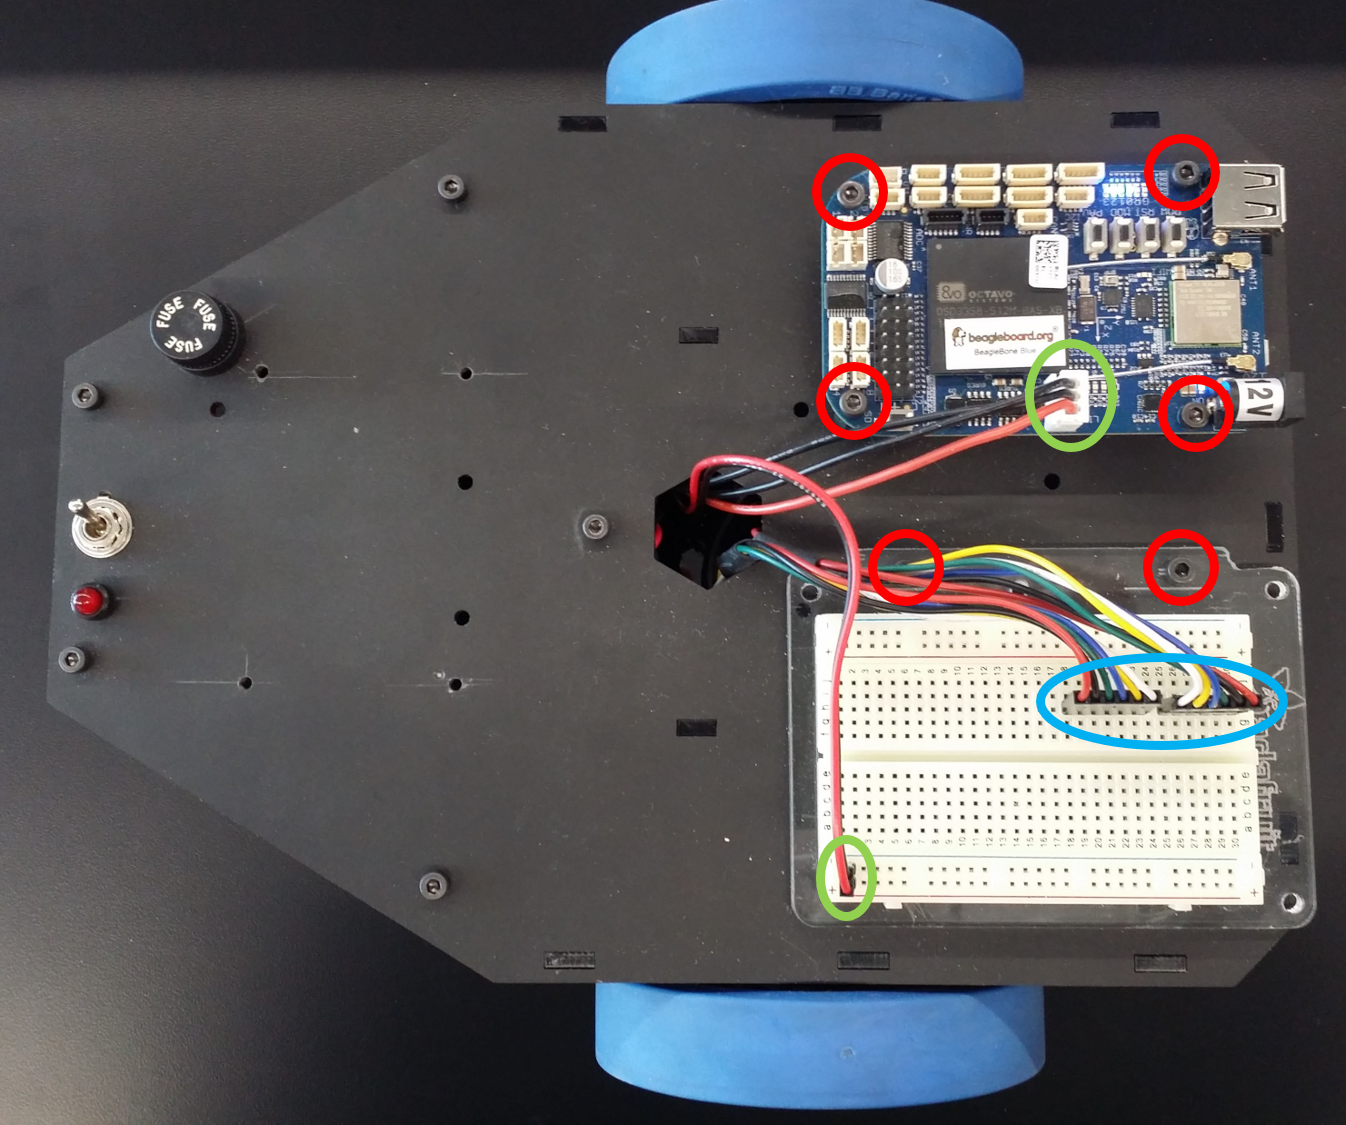
\includegraphics[width=3.6in]{figs/img/assembly/02-bbblueInstallation.png}
        \caption{BBBlue and Breadboard Installation}
        \label{fig:bbblueInstallation}
    \end{figure}

    \item Connect the motor terminals to the motor output channels on the BBBlue (left: ch1, right: ch2) using two 2-pin JST-ZH connectors. Connect the motor encoders to the encoder channels on the BBBlue (left: ch1, right: ch2) using two 4-pin JST-SH connectors (Fig. \ref{fig:motorWiring}).
    \begin{figure}[H]
        \centering
        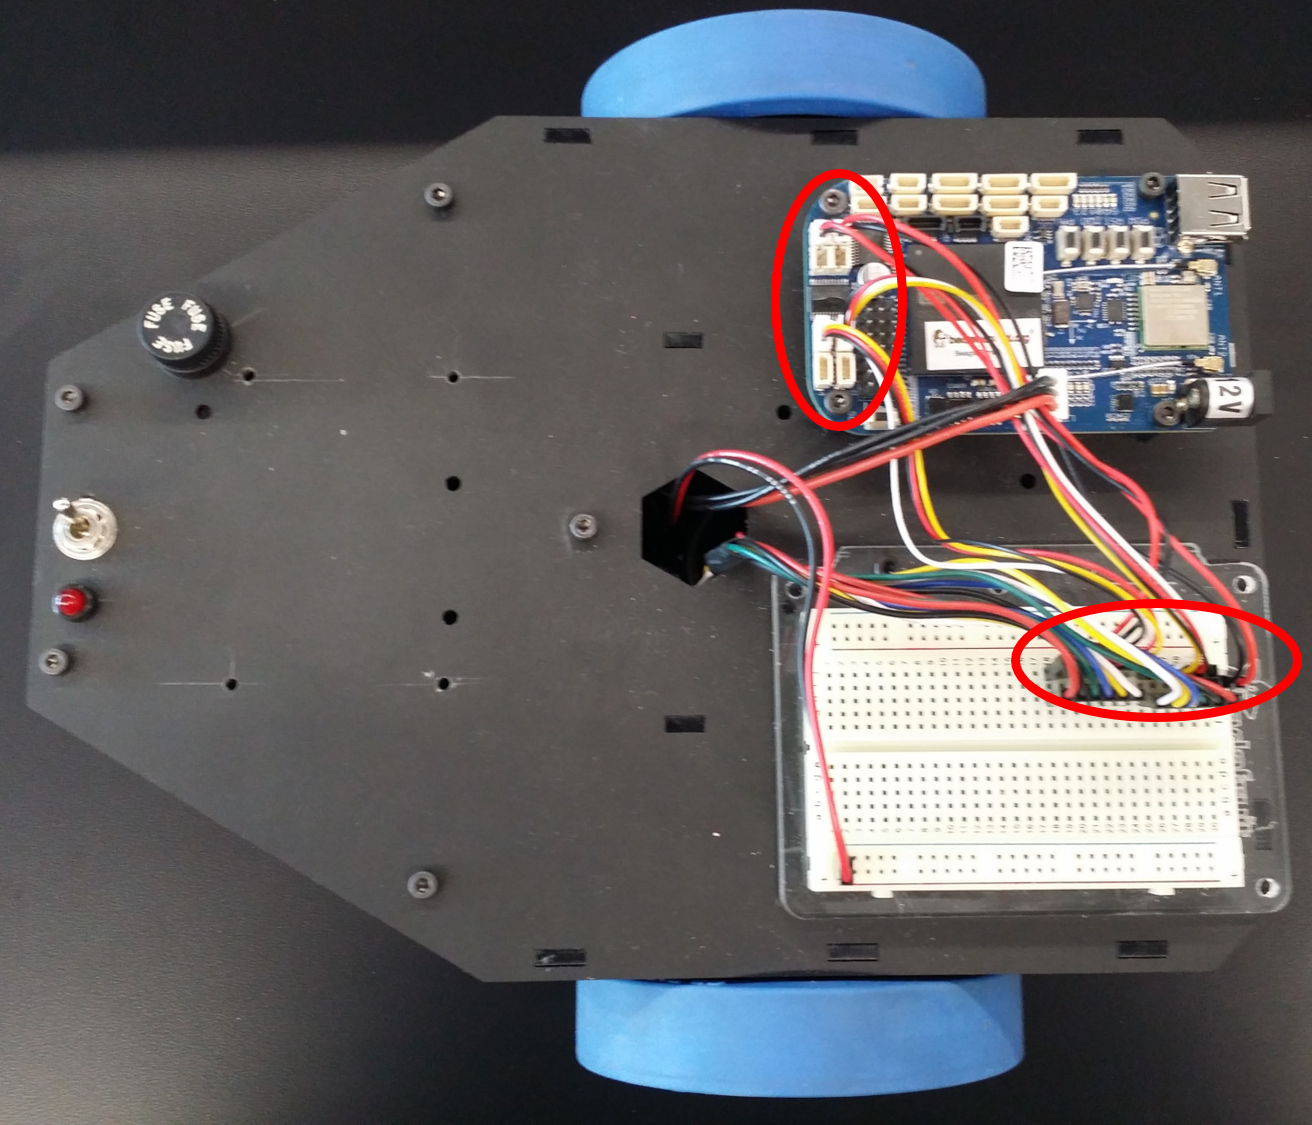
\includegraphics[width=3.6in]{figs/img/assembly/03-motorWiring.png}
        \caption{Motor Wiring}
        \label{fig:motorWiring}
    \end{figure}

    \item Prepare the stepper motor, the stepper motor bracket, four 6mm M3 screws, and four 8mm M3 screws (Fig. \ref{fig:stepperParts}).
    \begin{figure}[H]
        \centering
        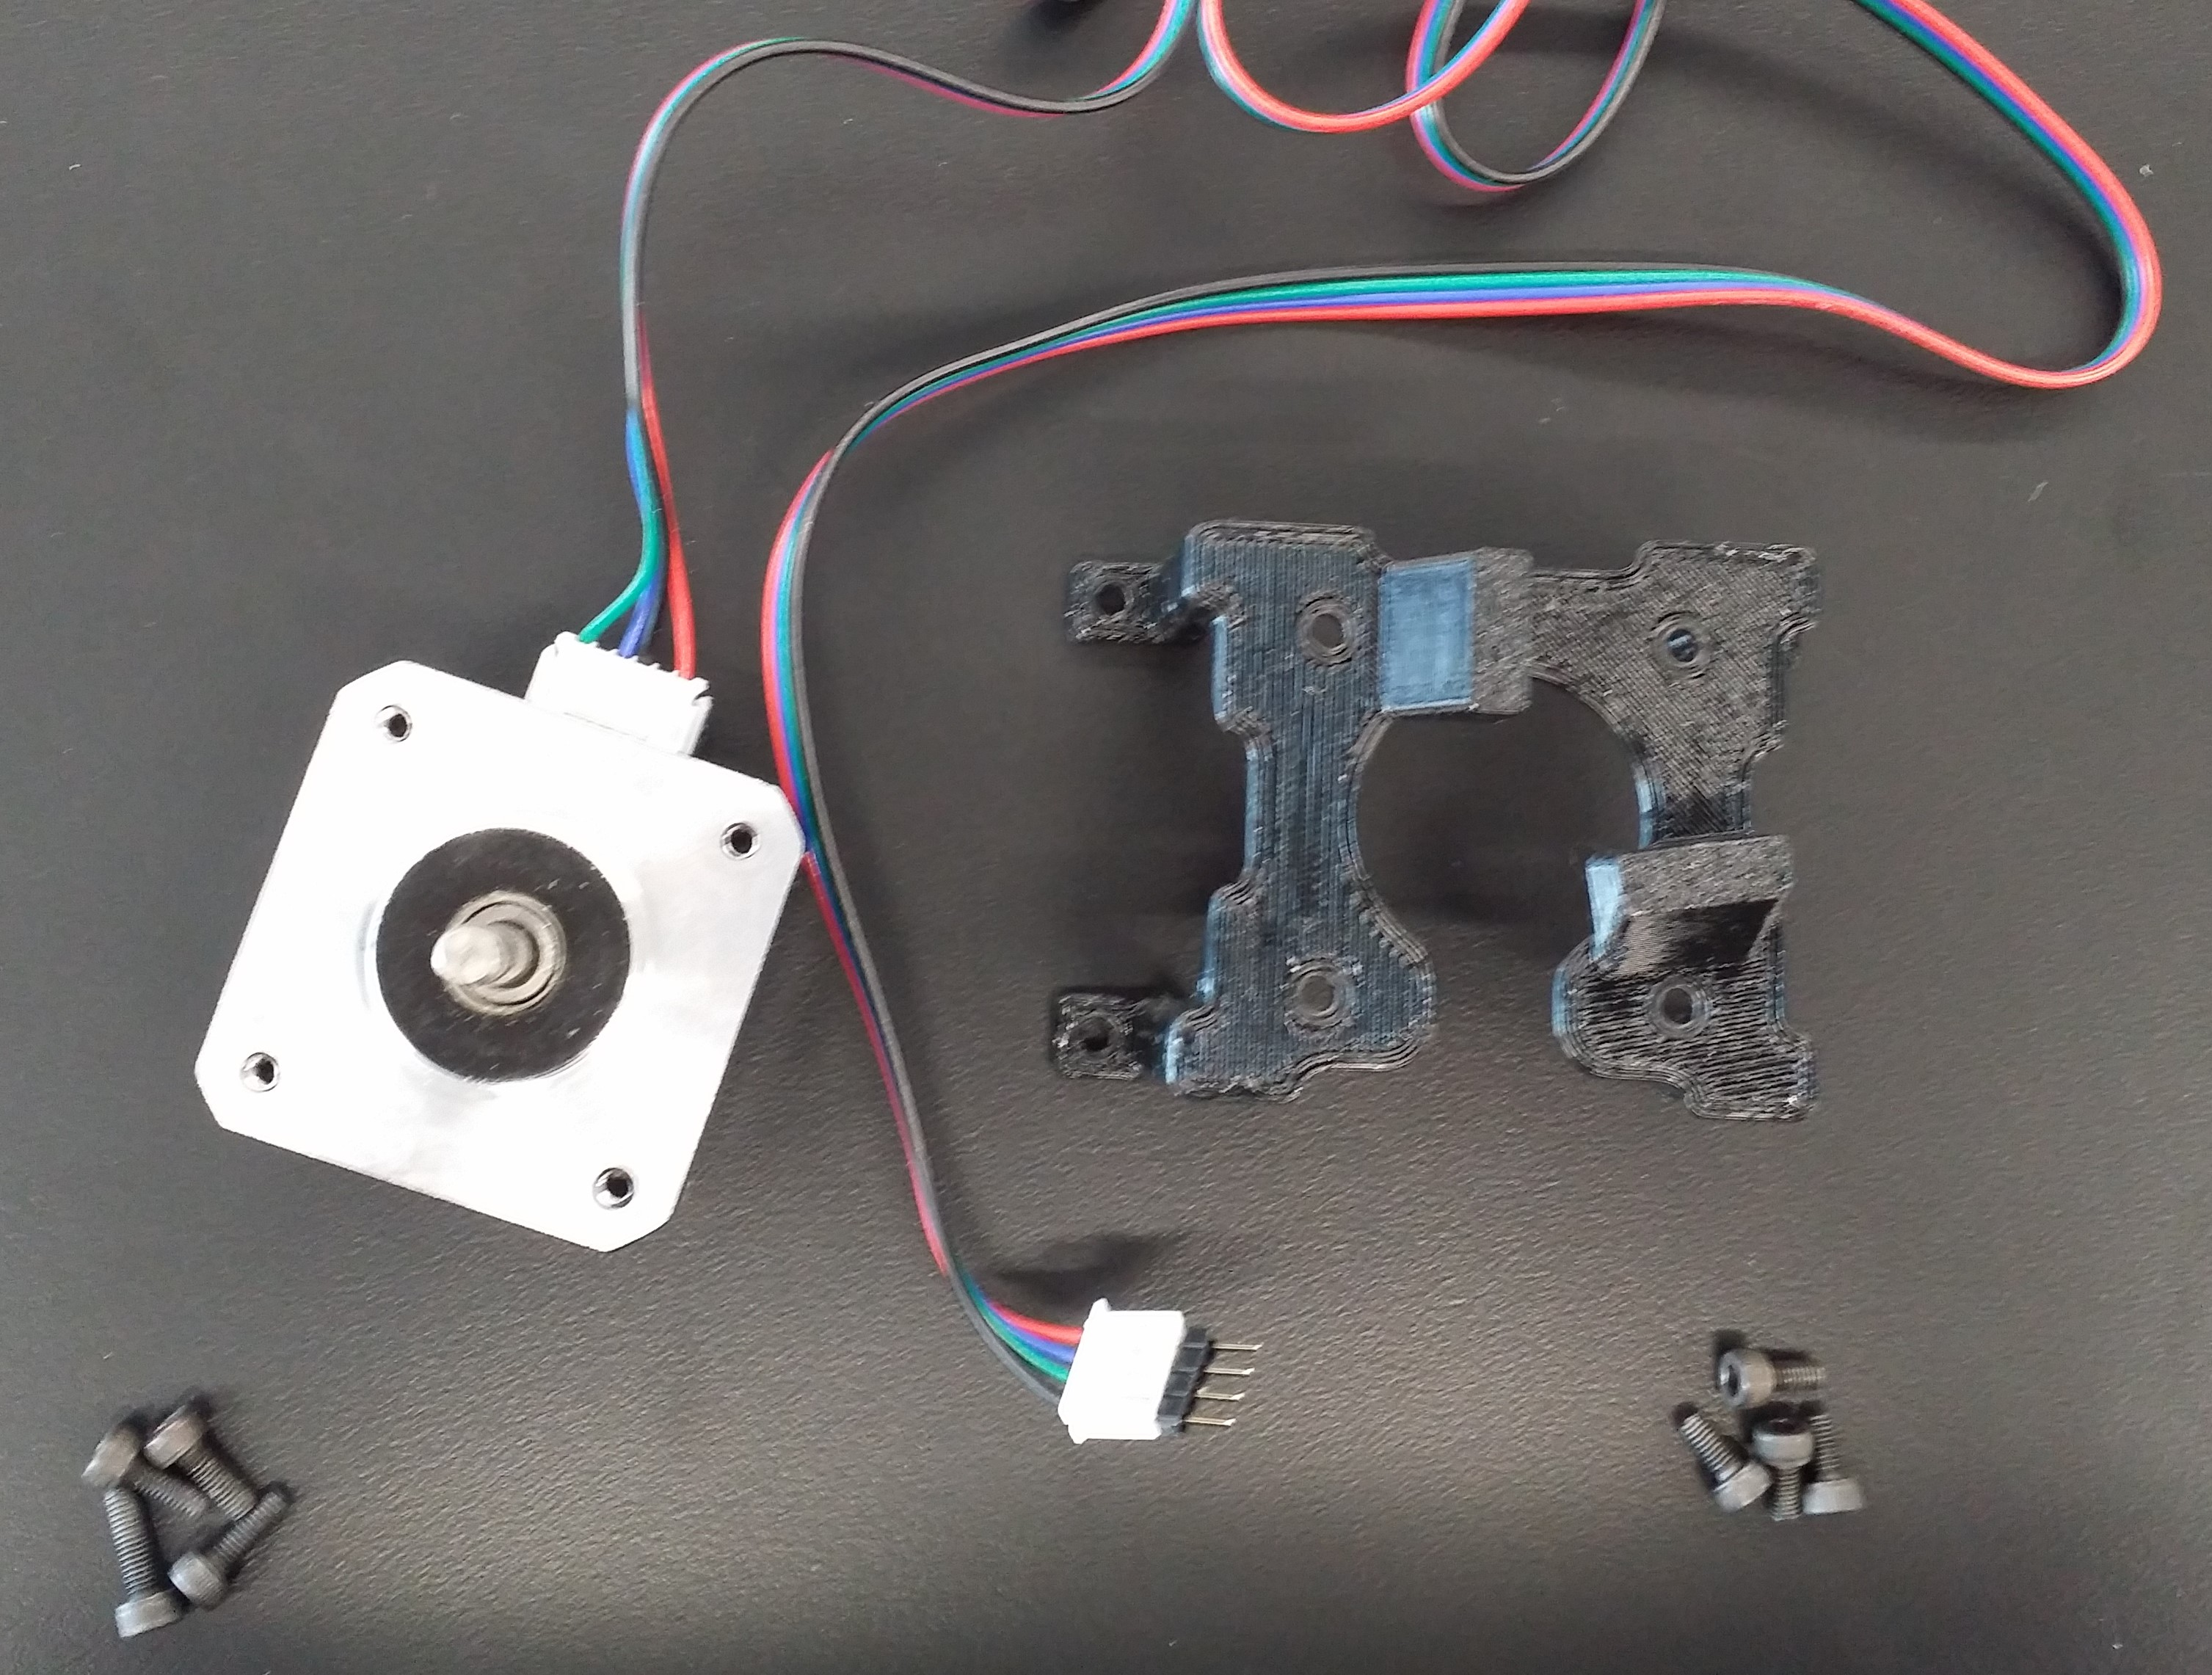
\includegraphics[width=4in]{figs/img/assembly/04-stepperParts.jpg}
        \caption{Stepper Motor Parts}
        \label{fig:stepperParts}
    \end{figure}

    \item Insert four 6mm M3 screws through the holes on the top of the bracket and secure the stepper motor to the stepper motor bracket by threading the screws into the holes in the stepper motor (Fig. \ref{fig:stepperAssembly}). Make sure the motor connector comes out on the side of the bracket with the notch.
    \begin{figure}[H]
        \centering
        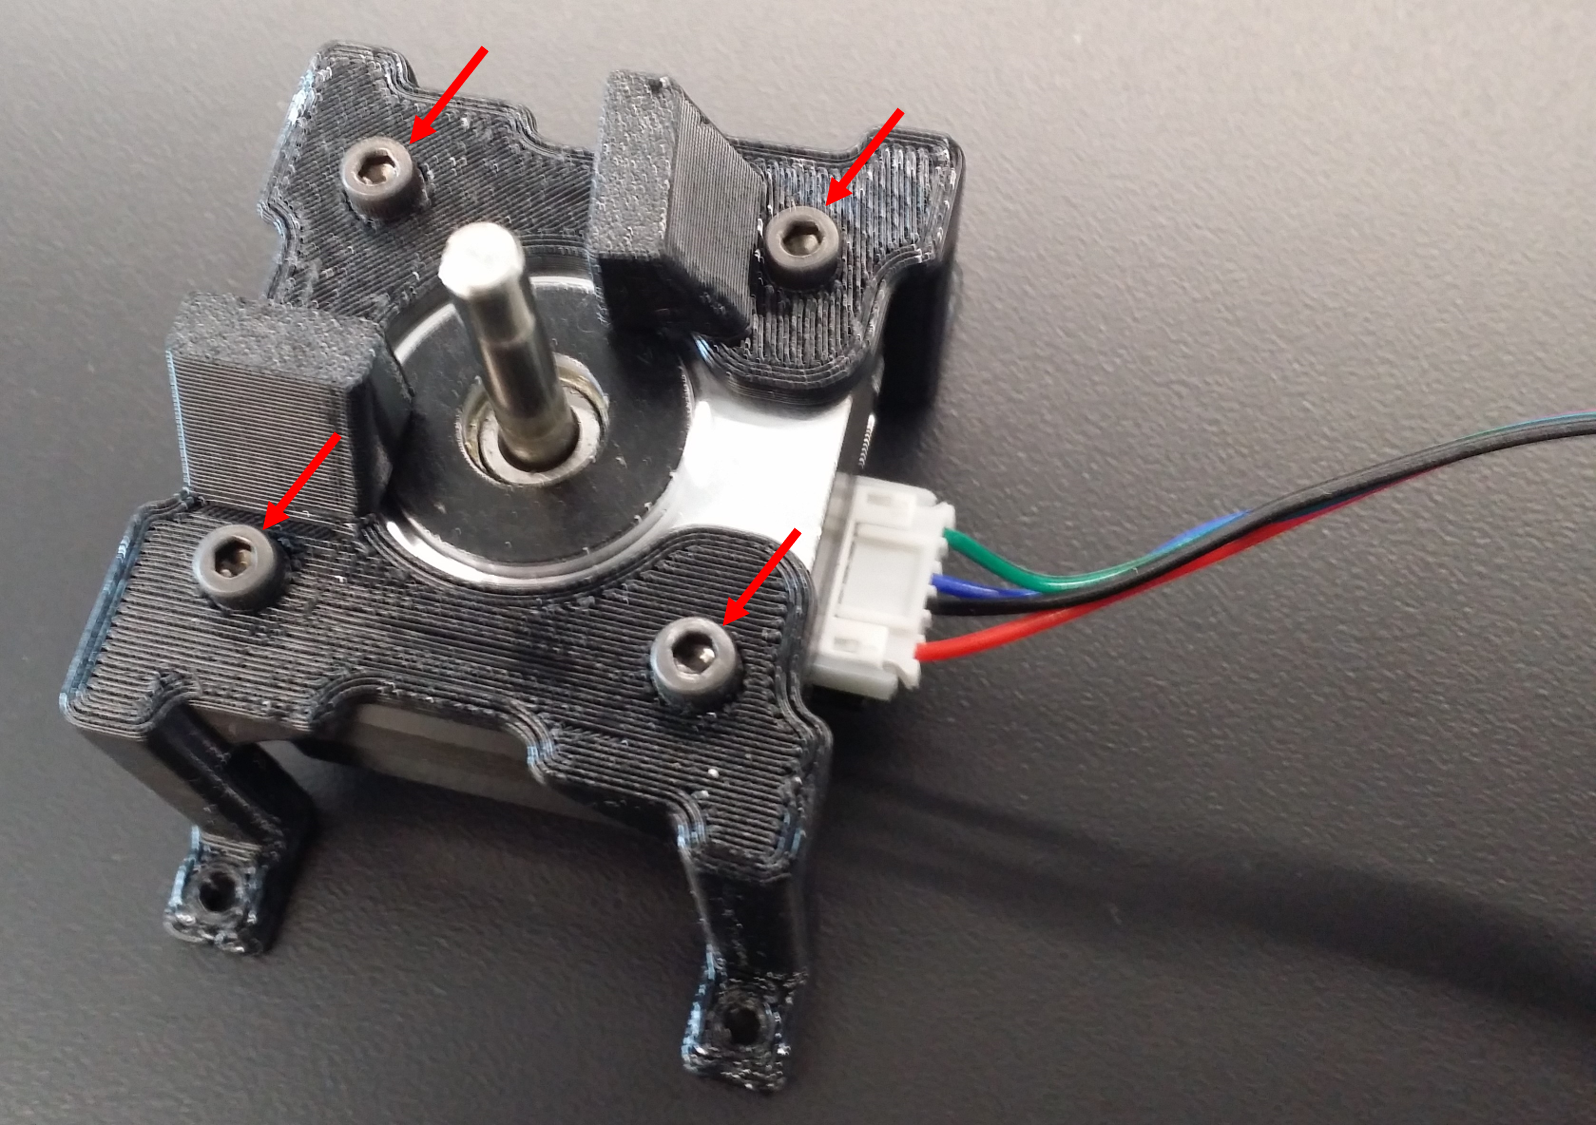
\includegraphics[width=4in]{figs/img/assembly/05-stepperAssembly.png}
        \caption{Mounting Stepper Motor onto Bracket}
        \label{fig:stepperAssembly}
    \end{figure}
    \pagebreak

    \item Insert four 8mm M3 screws through the holes in the feet of the bracket and secure the bracket to the Budget Bot (Fig. \ref{fig:stepperMounting}). Holes must be drilled in the Budget Bot Chassis to thread the screws into. Insert the stepper motor connector into the breadboard and tuck away the excess cable inside the Budget Bot.
    \begin{figure}[H]
        \centering
        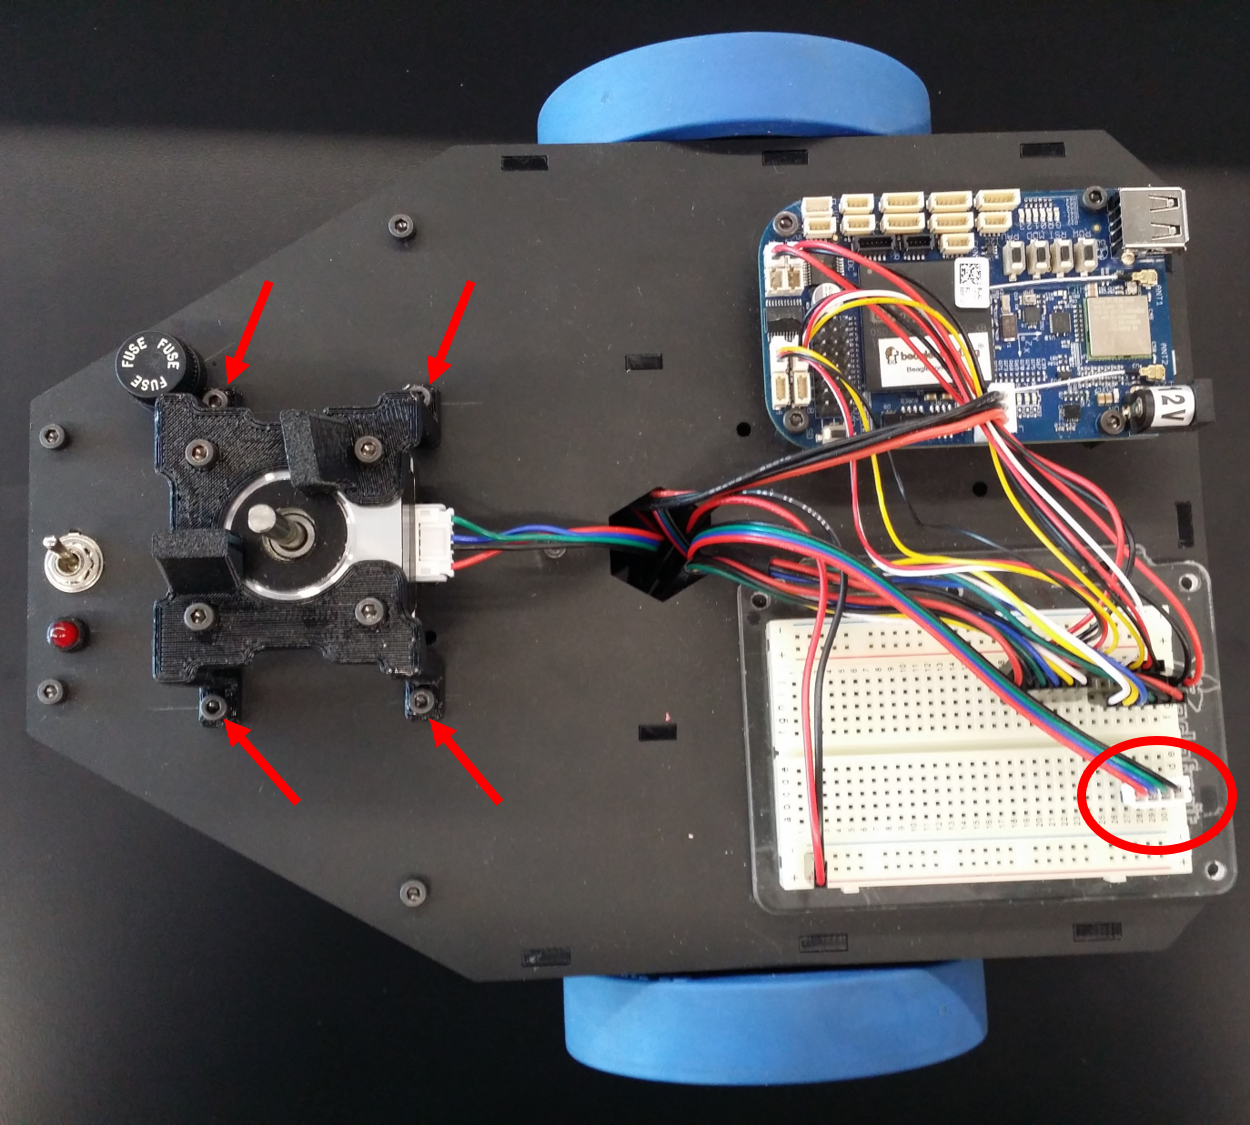
\includegraphics[width=3.7in]{figs/img/assembly/06-stepperMounting.png}
        \caption{Mounting Stepper Motor onto Budget Bot}
        \label{fig:stepperMounting}
    \end{figure}

    \item Using two 2-pin JST-ZH connectors, connect motor output channels 3 and 4 to the stepper motor windings (Fig. \ref{fig:stepperWiring}).
    \begin{figure}[H]
        \centering
        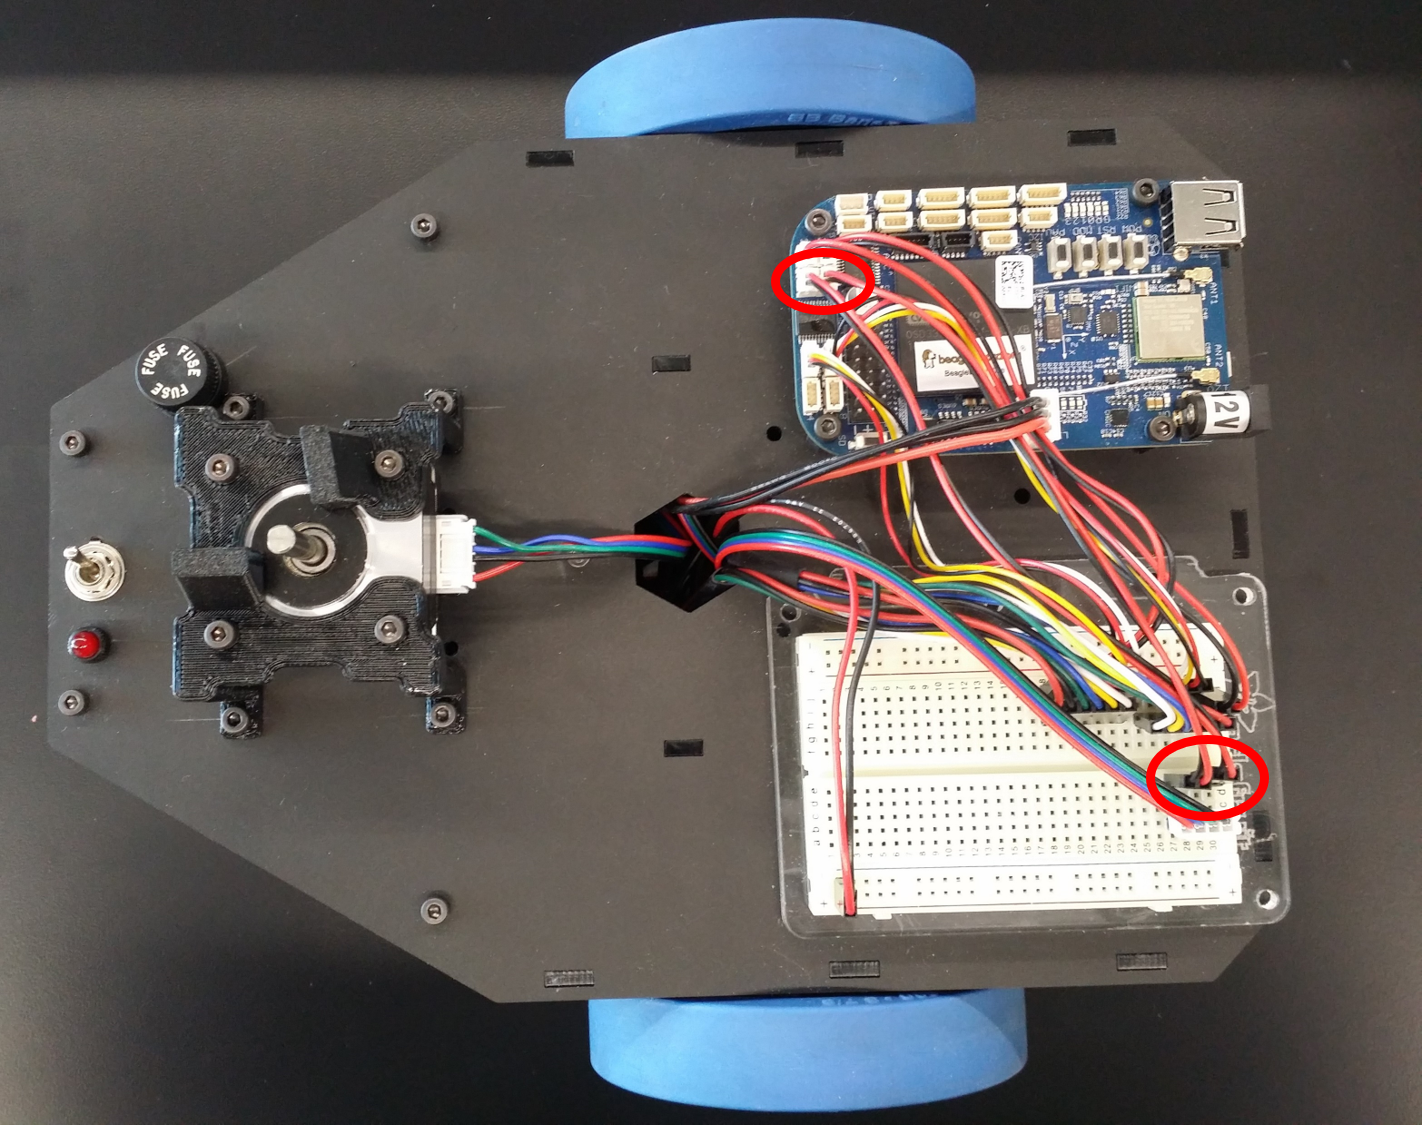
\includegraphics[width=4in]{figs/img/assembly/07-stepperWiring.png}
        \caption{Stepper Motor Wiring}
        \label{fig:stepperWiring}
    \end{figure}
    \pagebreak

    \item Insert a DG409DJ+ multiplexer across the center of the breadboard (Fig. \ref{fig:multiplexer}). Make sure the divot is toward the end of the breadboard to prevent mistakes during the rest of the assembly.
    \begin{figure}[H]
        \centering
        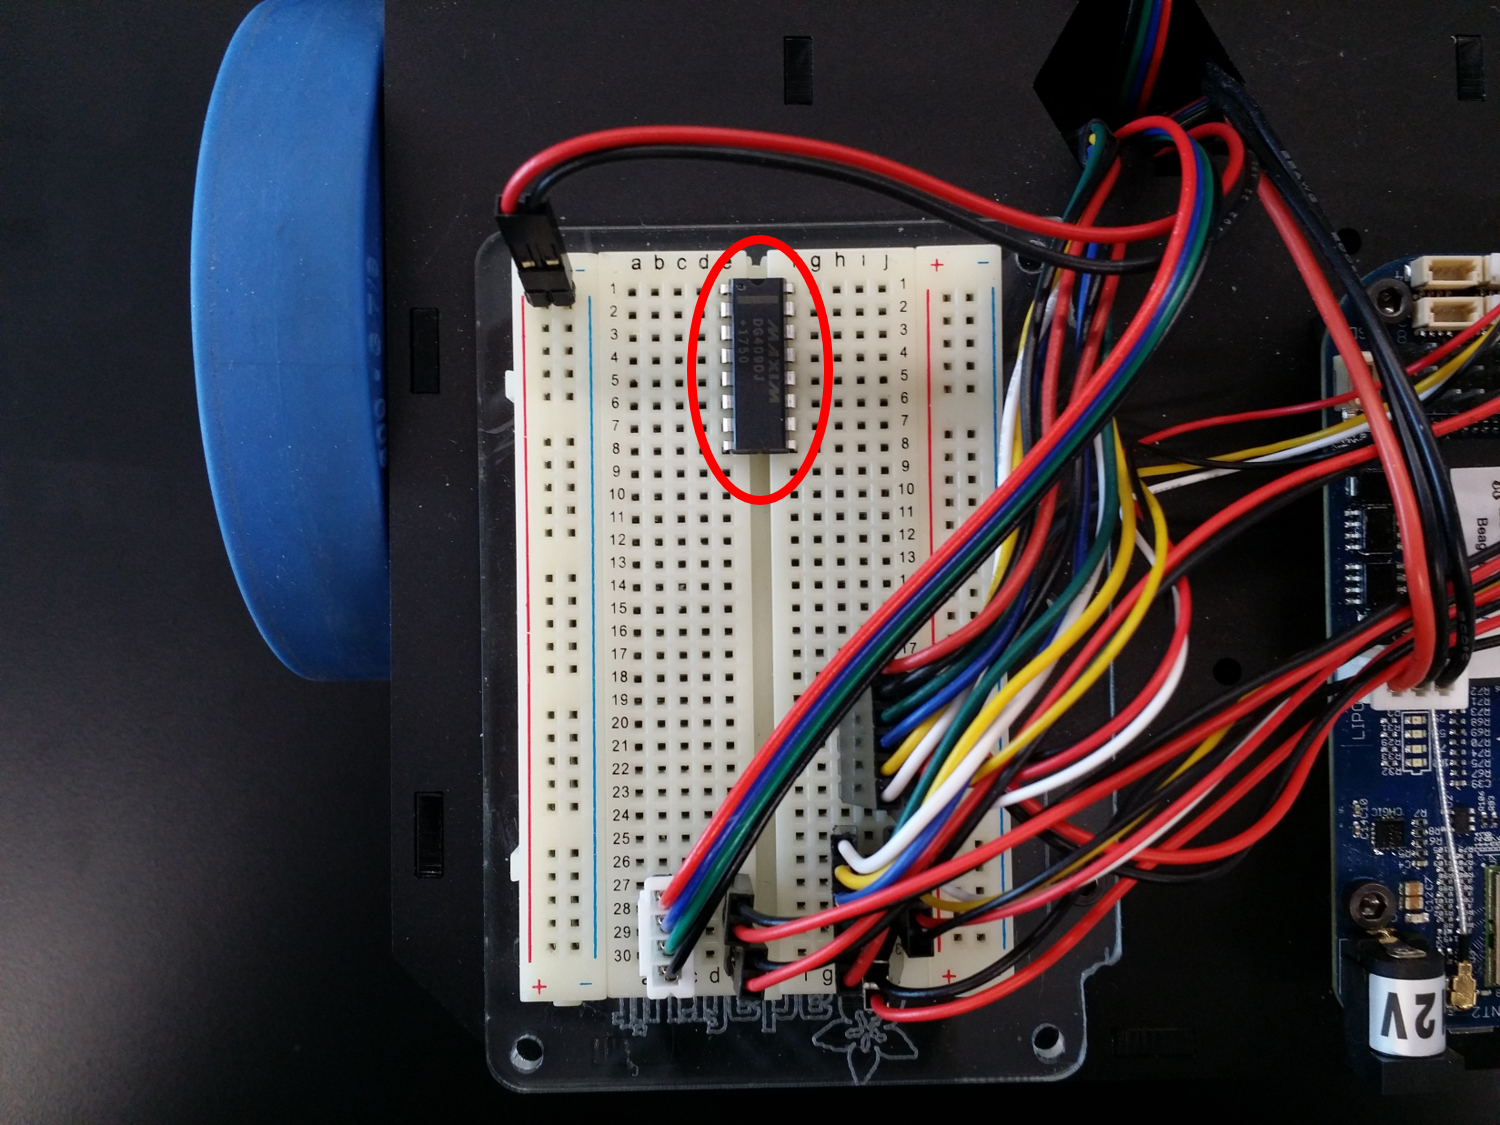
\includegraphics[width=4.2in]{figs/img/assembly/08-multiplexer.png}
        \caption{Multiplexer Installation}
        \label{fig:multiplexer}
    \end{figure}

    \item Connect battery power to the multiplexer by connecting V+ to pin 14 and GND to pin 15 of the multiplexer (Fig. \ref{fig:multiplexerPower}).
    \begin{figure}[H]
        \centering
        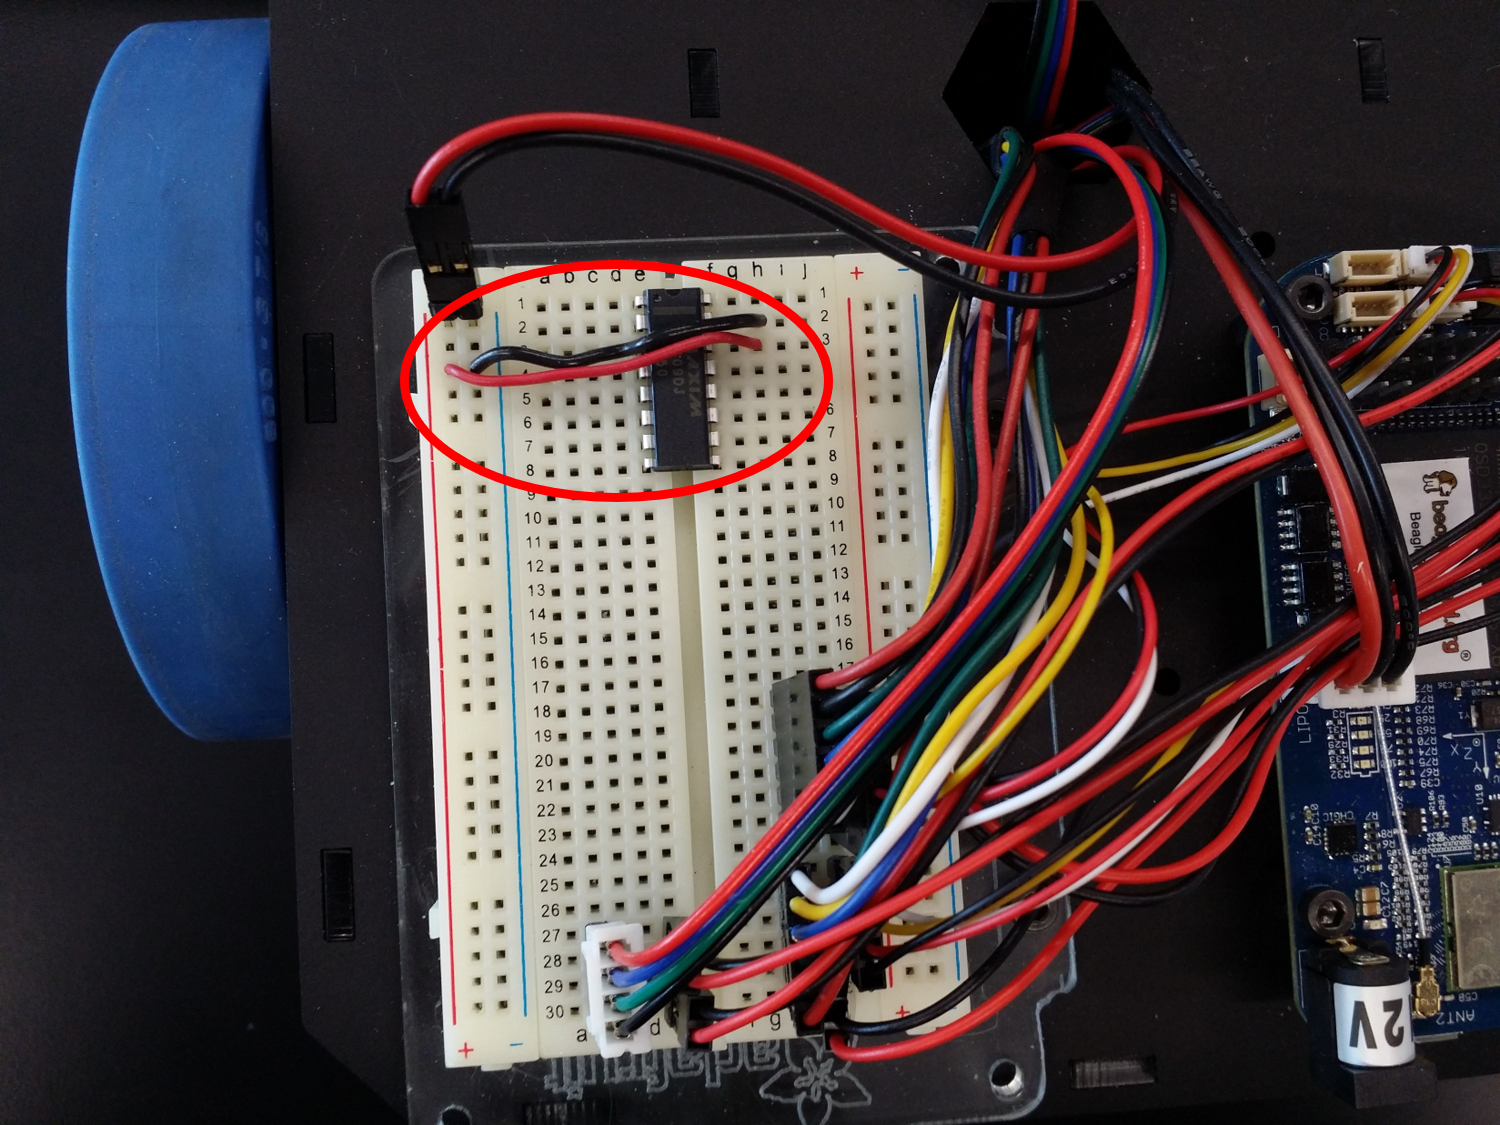
\includegraphics[width=4.2in]{figs/img/assembly/09-multiplexerPower.png}
        \caption{Powering the Multiplexer}
        \label{fig:multiplexerPower}
    \end{figure}
    \pagebreak

    \item Insert an LM1117 3.3V regulator into the breadboard. Place a 10\textmu F capacitor between the output terminal and ground. Connect the ground terminal to the battery ground and the input power terminal to the battery V+ (Fig. \ref{fig:regulator})
    \begin{figure}[H]
        \centering
        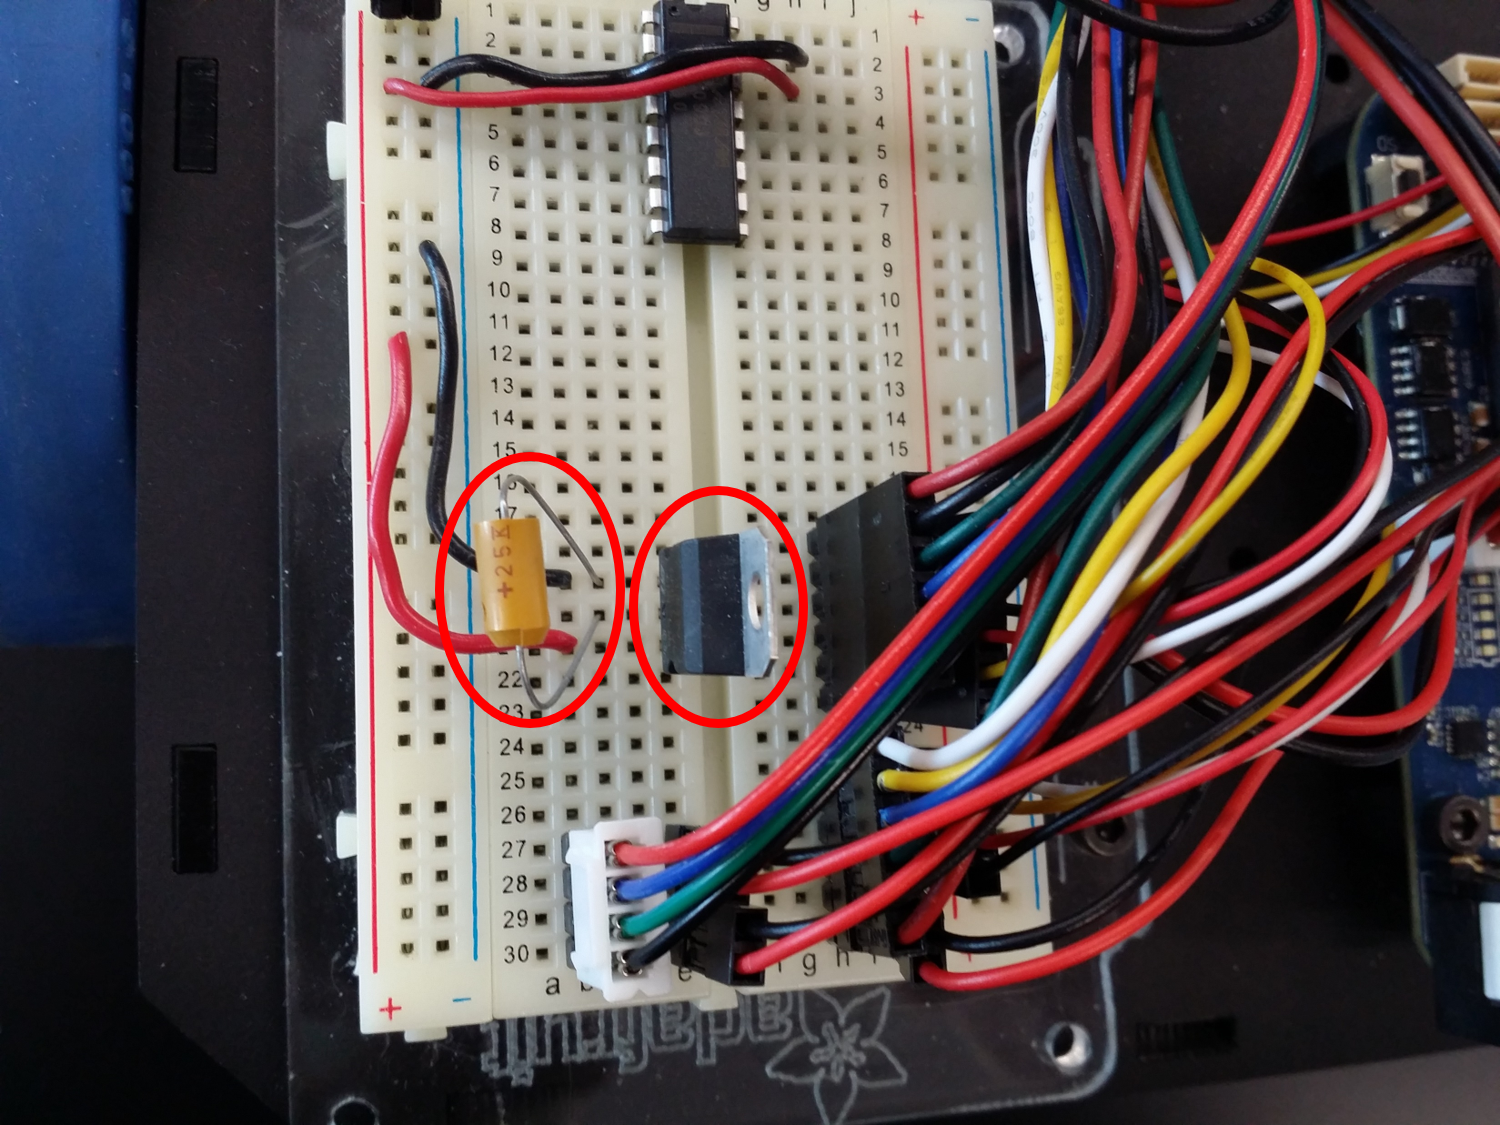
\includegraphics[width=3.8in]{figs/img/assembly/10-regulatorWiring.png}
        \caption{Regulator Installation}
        \label{fig:regulator}
    \end{figure}

    \item Connect +3.3V from GPIO1 to pin 2 on the multiplexer (Fig. \ref{fig:multiplexerWiring}, red arrows). Connect GPIO1 pins 1 and 2 to multiplexer pins 1 and 16, respectively (Fig. \ref{fig:multiplexerWiring}, green and orange arrows). Connect UART1 TX and RX to multiplexer pins 8 and 9, respectively (Fig. \ref{fig:multiplexerWiring}, yellow and purple arrows). Finally, connect UART5 TX and RX into the breadboard (Fig. \ref{fig:multiplexerWiring}, blue arrows).
    \begin{figure}[H]
        \centering
        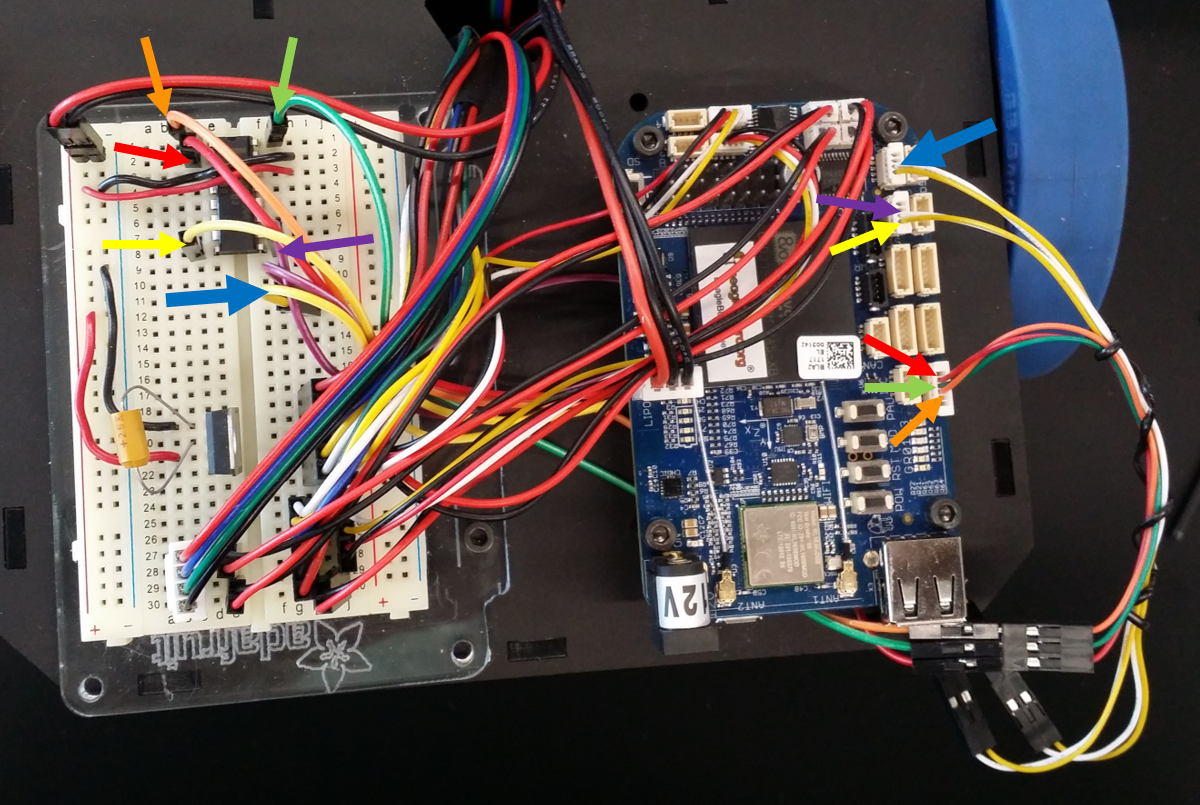
\includegraphics[width=4.8in]{figs/img/assembly/11-multiplexerBBBlueWiring.png}
        \caption{Connecting the Multiplexer to the BBBlue}
        \label{fig:multiplexerWiring}
    \end{figure}
    \pagebreak

    \item Prepare the reflector dishes, top plate, and bottom frame. Also prepare some 8mm and 10mm M3 screws and some M3 nuts (Fig. \ref{fig:reflectorParts}).
    \begin{figure}[H]
        \centering
        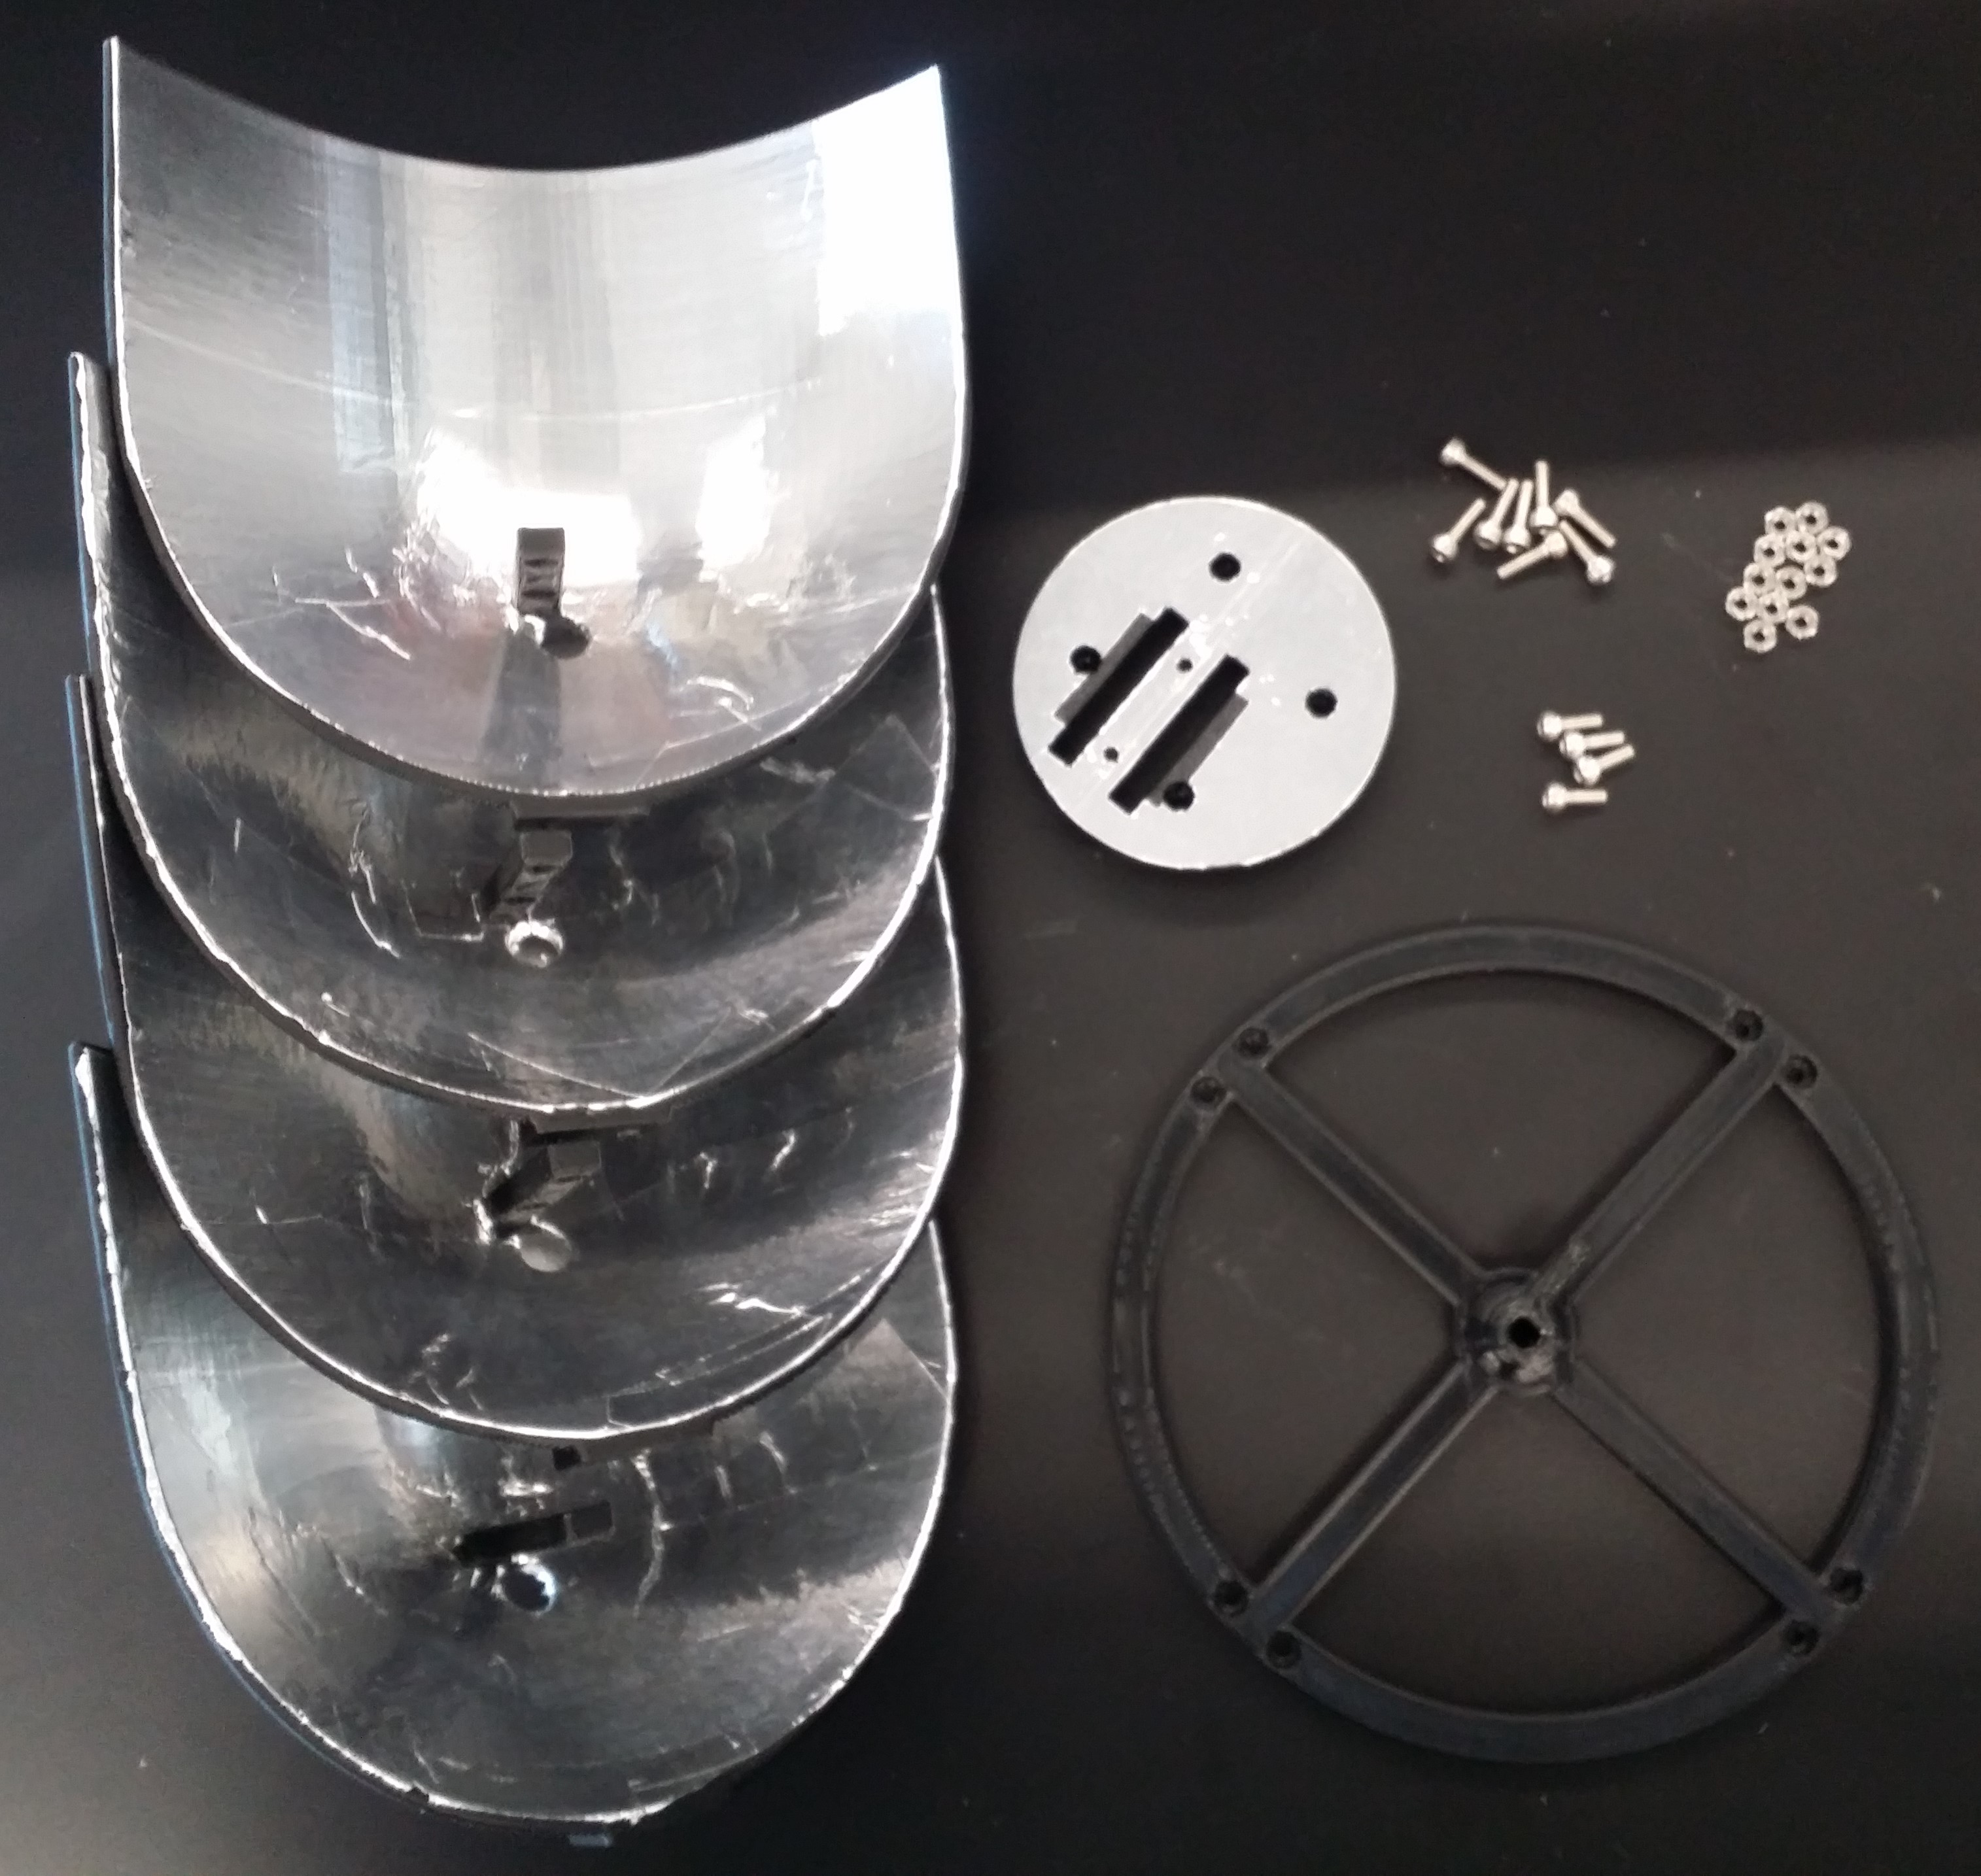
\includegraphics[width=4.4in]{figs/img/assembly/12-reflectorParts.jpg}
        \caption{Reflector Parts}
        \label{fig:reflectorParts}
    \end{figure}

    \item Insert an M3 nut into the slot at the top of one of the reflector dishes (Fig. \ref{fig:reflectorTopNut}).
    \begin{figure}[H]
        \centering
        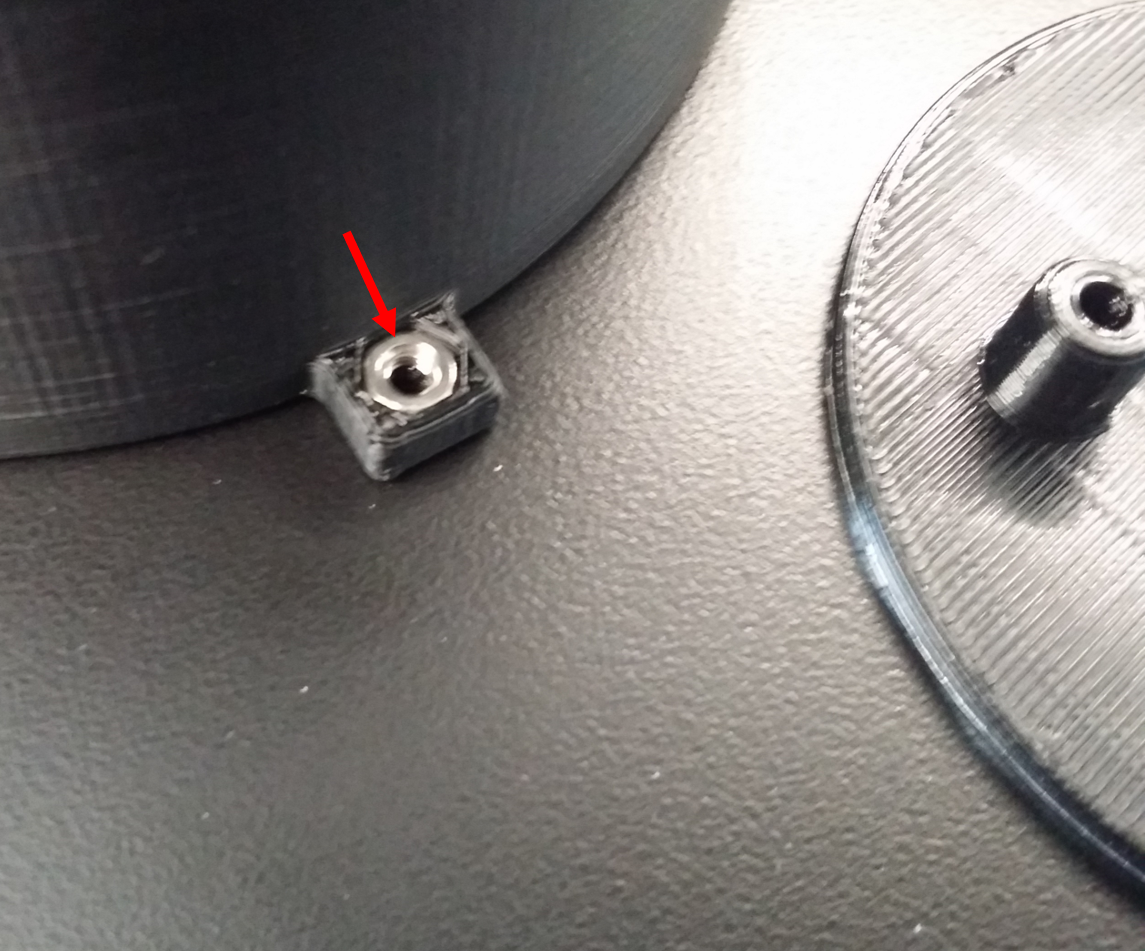
\includegraphics[width=3.6in]{figs/img/assembly/13-reflectorTopNut.png}
        \caption{Top Reflector Nut}
        \label{fig:reflectorTopNut}
    \end{figure}
    \pagebreak

    \item Attach the top plate using an 8mm M3 screw (Fig. \ref{fig:reflectorTopPlate}).
    \begin{figure}[H]
        \centering
        \includegraphics[width=4.1in]{figs/img/assembly/14-reflectorTopPlate.jpg}
        \caption{Attaching Top Plate}
        \label{fig:reflectorTopPlate}
    \end{figure}

    \item Repeat steps 13 and 14 to attach all of the reflector dishes to the top plate (Fig. \ref{fig:finishedTopPlate}).
    \begin{figure}[H]
        \centering
        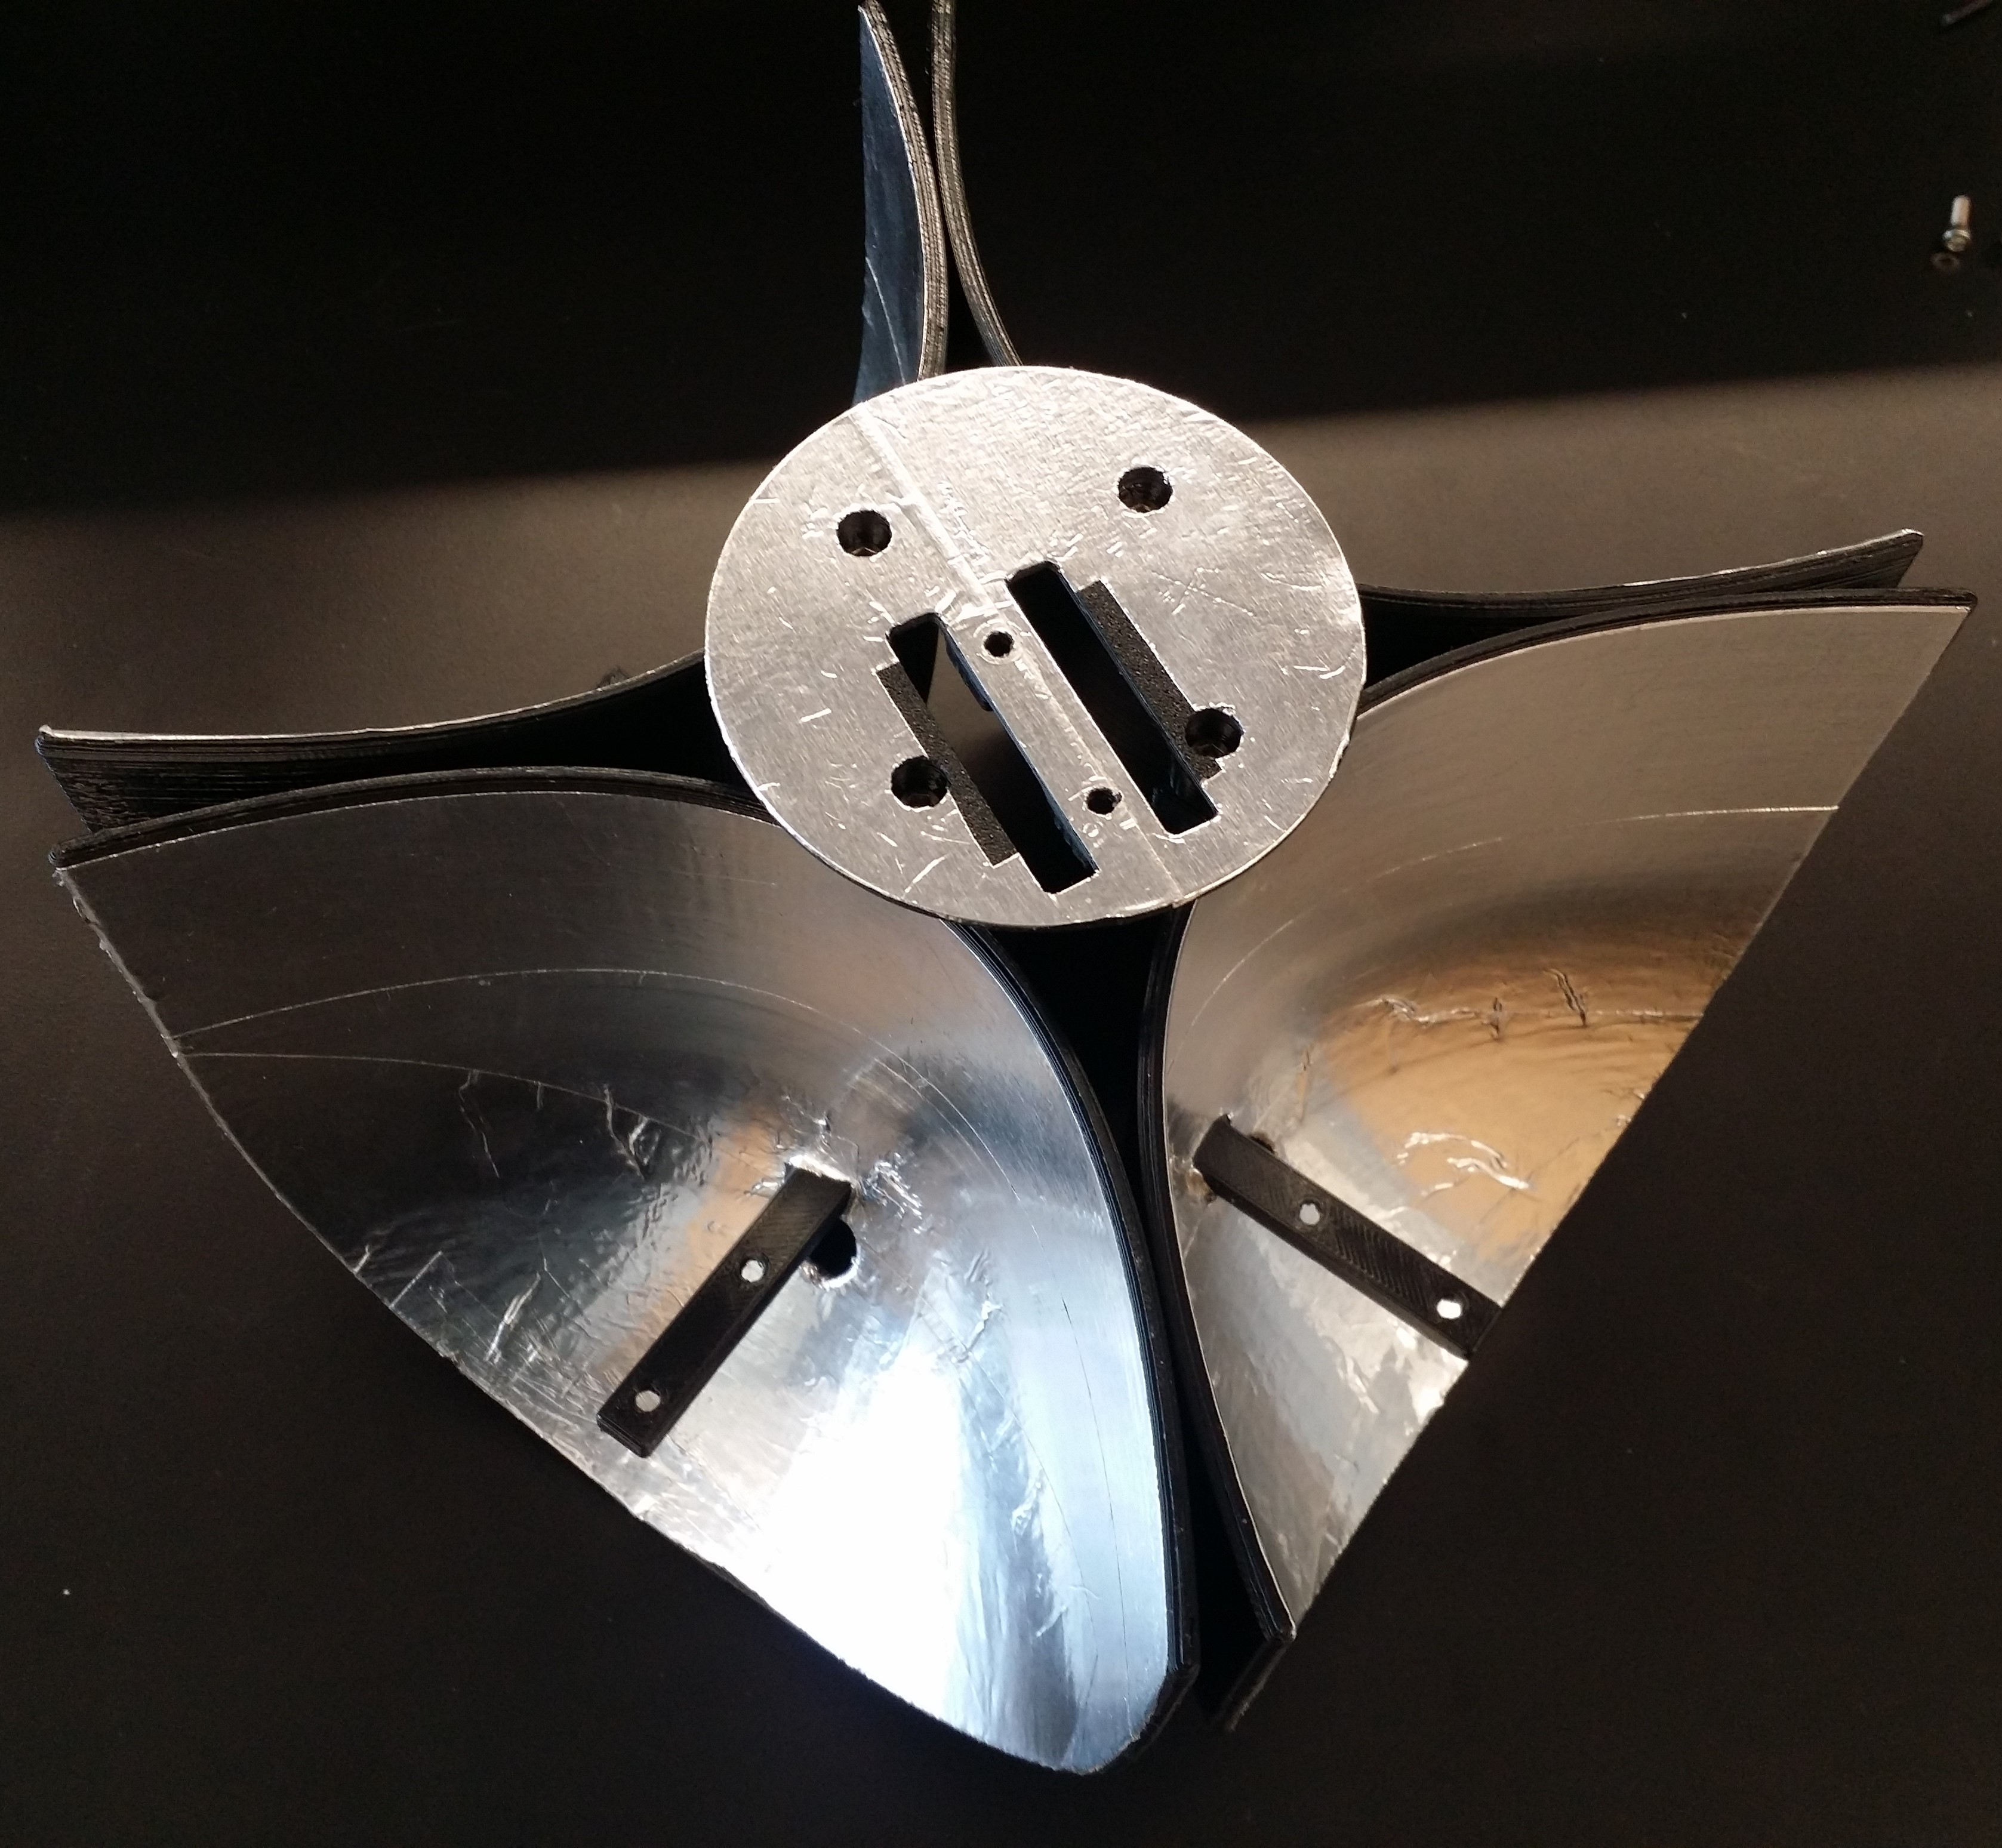
\includegraphics[width=4.1in]{figs/img/assembly/15-finishedReflectorTopPlate.jpg}
        \caption{Finished Top Plate}
        \label{fig:finishedTopPlate}
    \end{figure}
    \pagebreak

    \item Insert wires from the bottom of the reflectors up through the left slot (when viewed from above) and connect them to the VCC (red), DOUT (purple), DIN (yellow), and VSS (black) pins of an XBee adapter board (Fig. \ref{fig:topXBeeWiring}).
    \begin{figure}[H]
        \centering
        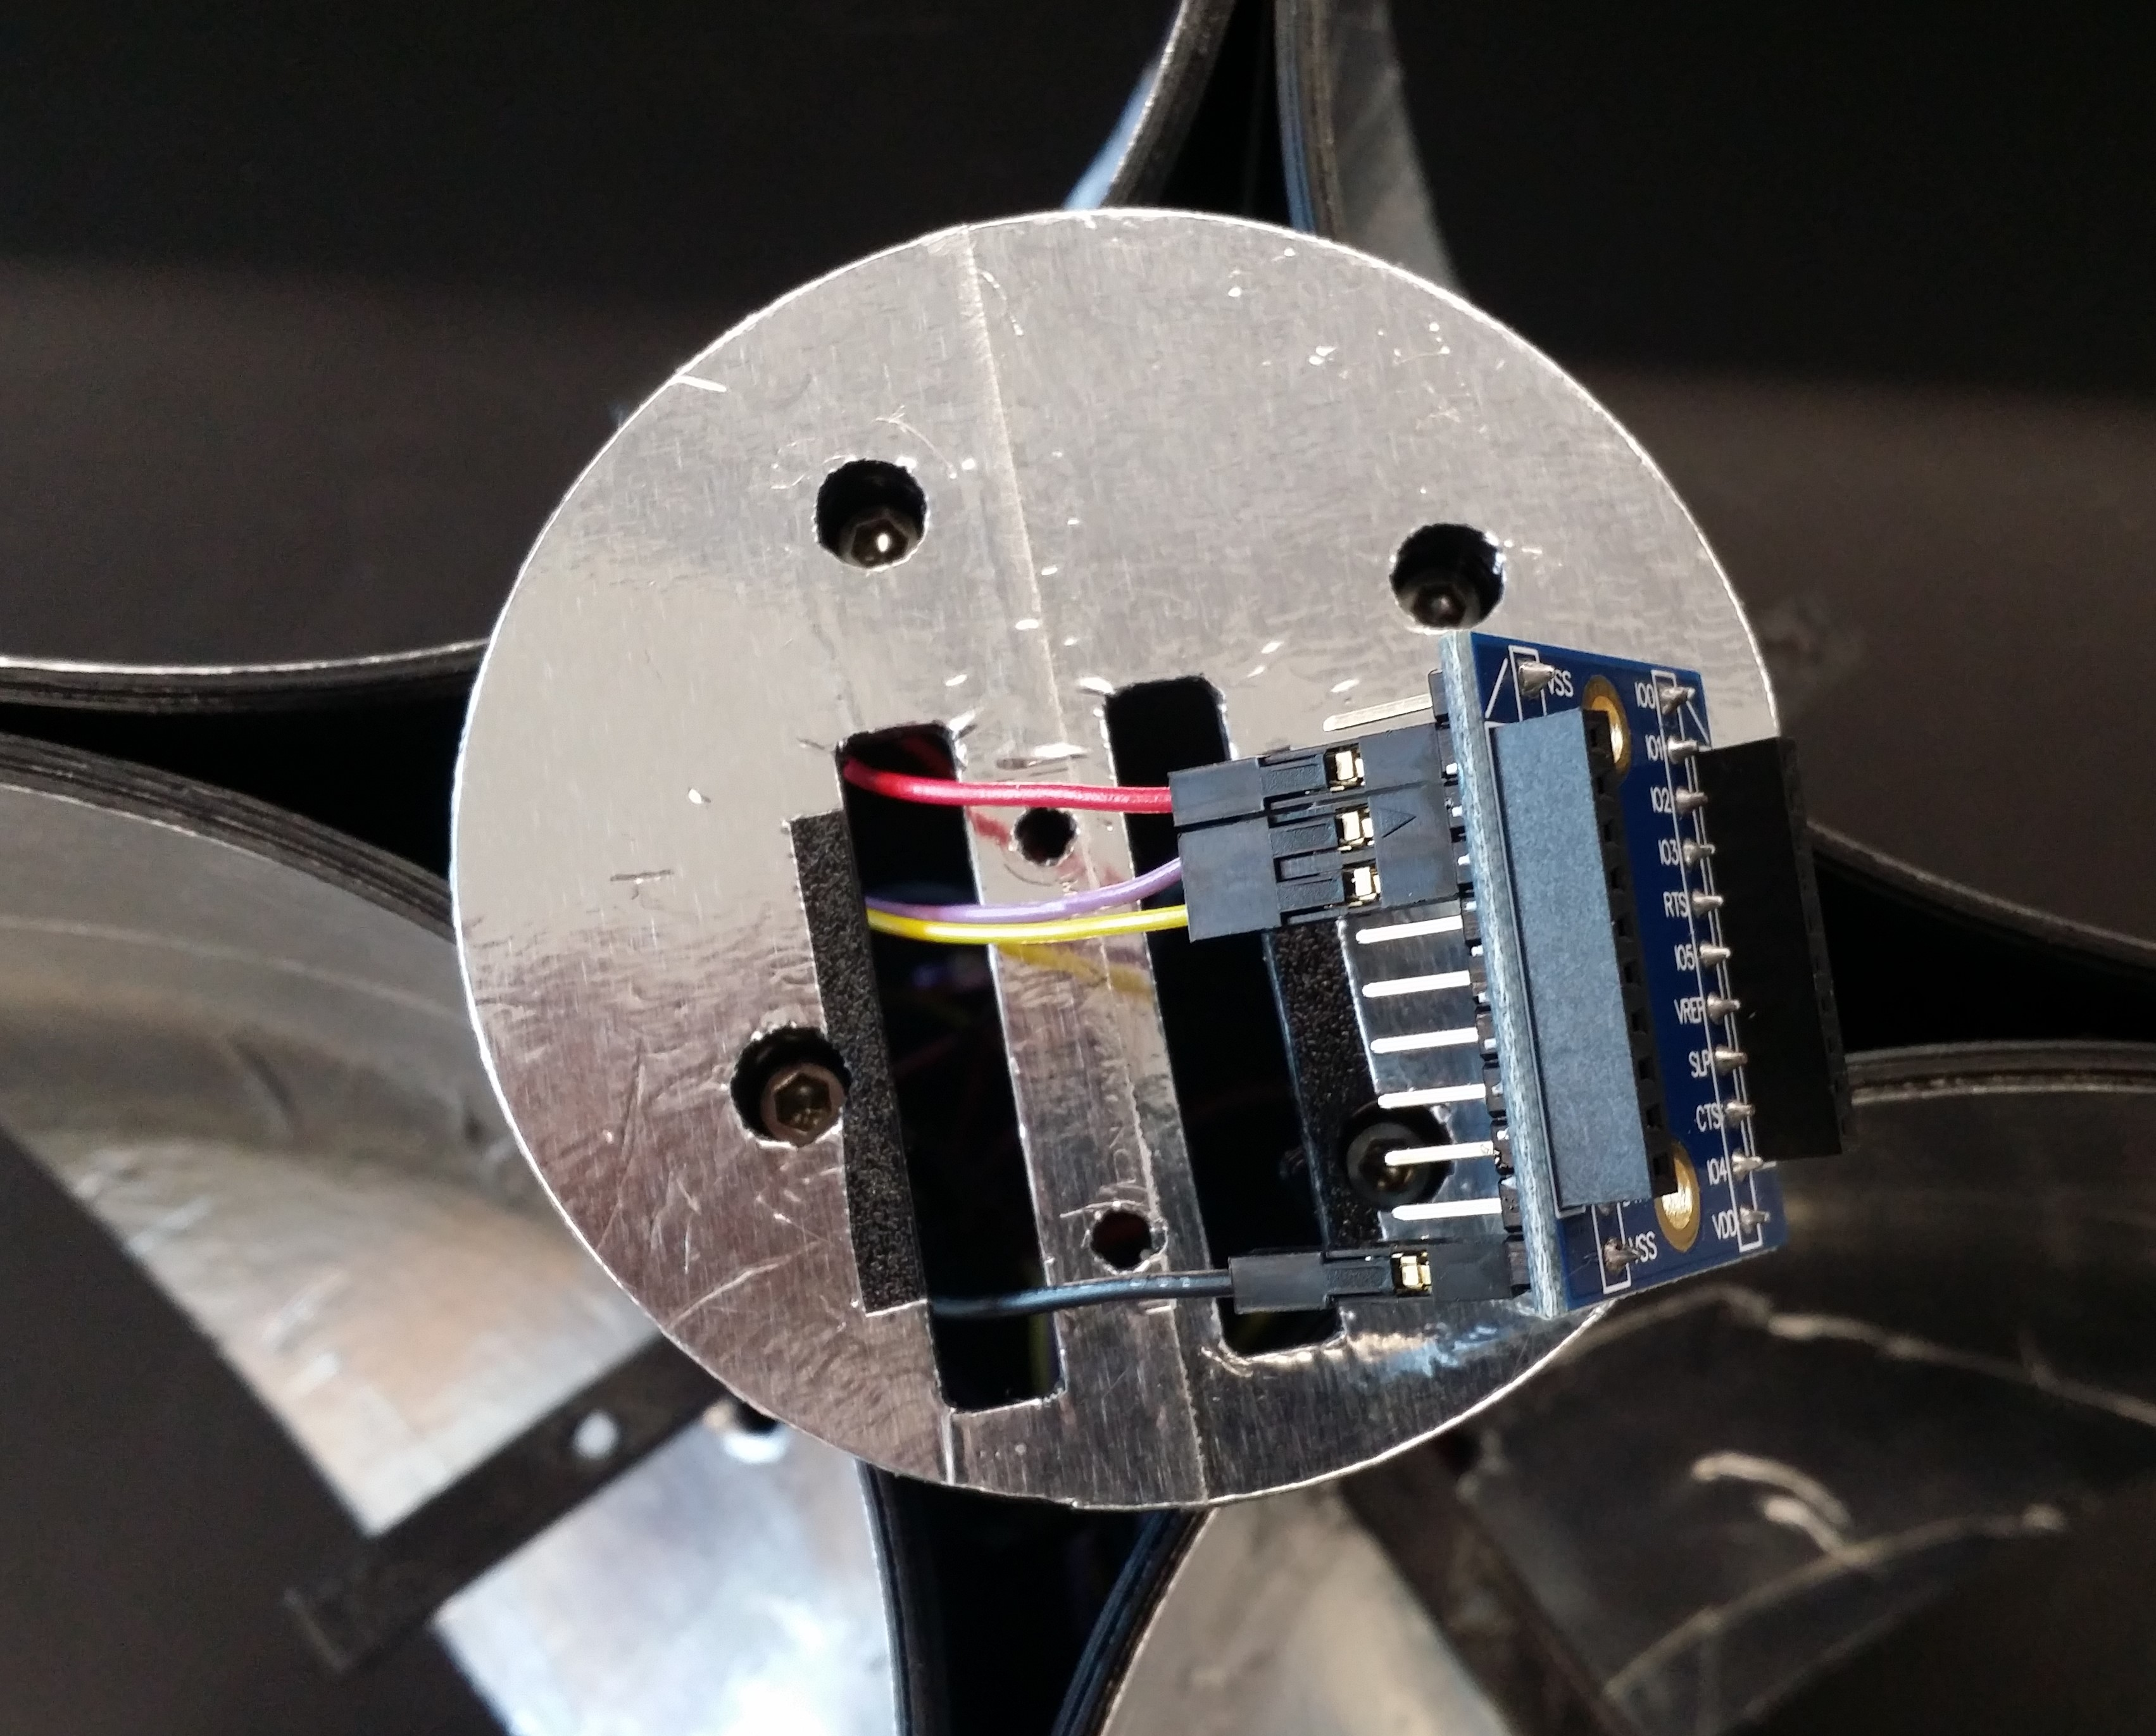
\includegraphics[width=4.2in]{figs/img/assembly/16-topXBeeWiring.jpg}
        \caption{Wiring for Top XBee}
        \label{fig:topXBeeWiring}
    \end{figure}

    \item Insert two M3 nuts into the slots on the underside of the top plate (Fig. \ref{fig:topXBeeNuts}).
    \begin{figure}[H]
        \centering
        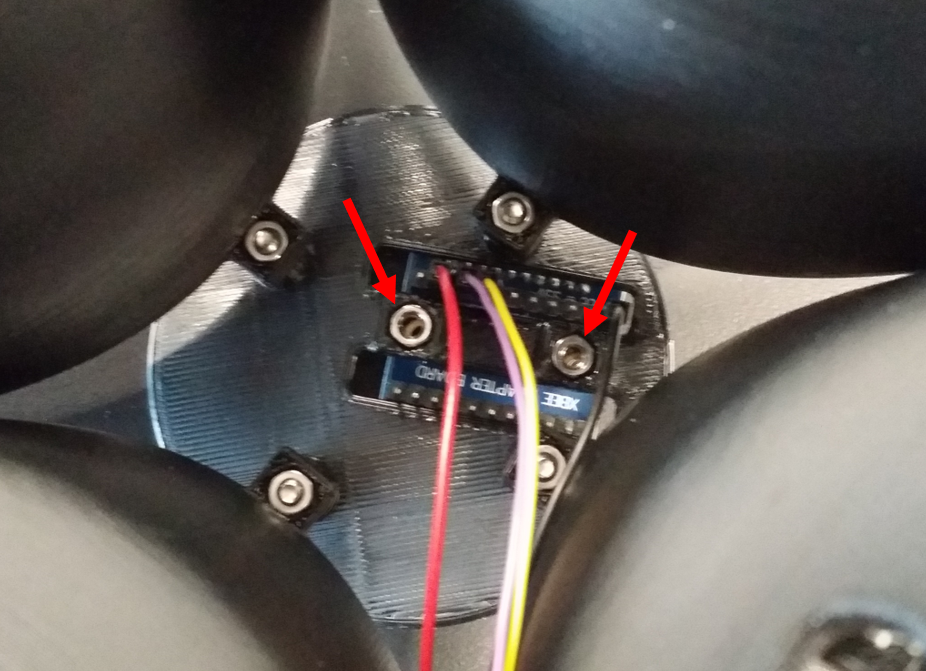
\includegraphics[width=4.2in]{figs/img/assembly/17-topXBeeNuts.png}
        \caption{Nuts for top XBee}
        \label{fig:topXBeeNuts}
    \end{figure}
    \pagebreak

    \item Attach the XBee adapter board to the top plate using two 8mm M3 screws (Fig. \ref{fig:topXBeeMounting}).
    \begin{figure}[H]
        \centering
        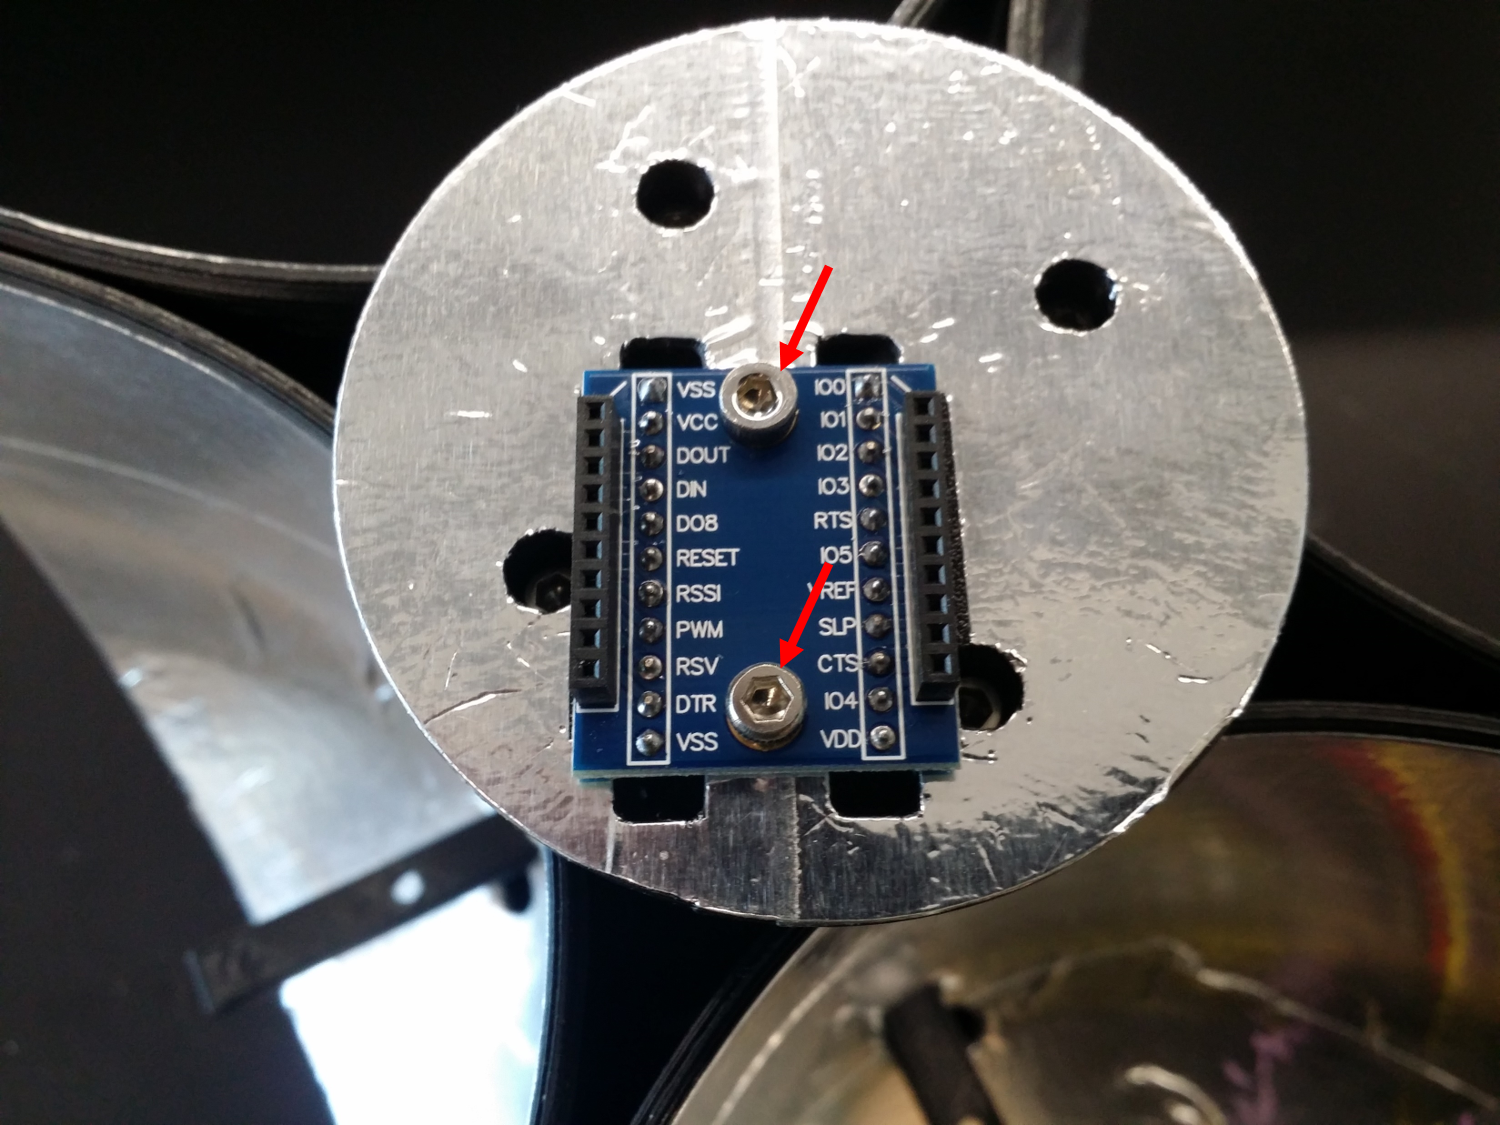
\includegraphics[width=4.2in]{figs/img/assembly/18-topXBeeMounting.png}
        \caption{Mounting the Top XBee}
        \label{fig:topXBeeMounting}
    \end{figure}

    \item Insert wires through the back of a reflector dish and connect them to the VCC (red), DOUT (purple), DIN (yellow), and VSS (black) pins of an XBee adapter board (Fig. \ref{fig:sideXBeeWiring}). It is useful to number the purple and yellow wires at both ends with the reflector number. The reflectors should be numbered 1 through 4 going clockwise.
    \begin{figure}[H]
        \centering
        \includegraphics[width=4.2in]{figs/img/assembly/19-sideXBeeWiring.jpg}
        \caption{Wiring a Side XBee}
        \label{fig:sideXBeeWiring}
    \end{figure}
    \pagebreak

    \item Insert two M3 nuts into the underside of the support protruding from the reflector (Fig. \ref{fig:sideXBeeNuts})
    \begin{figure}[H]
        \centering
        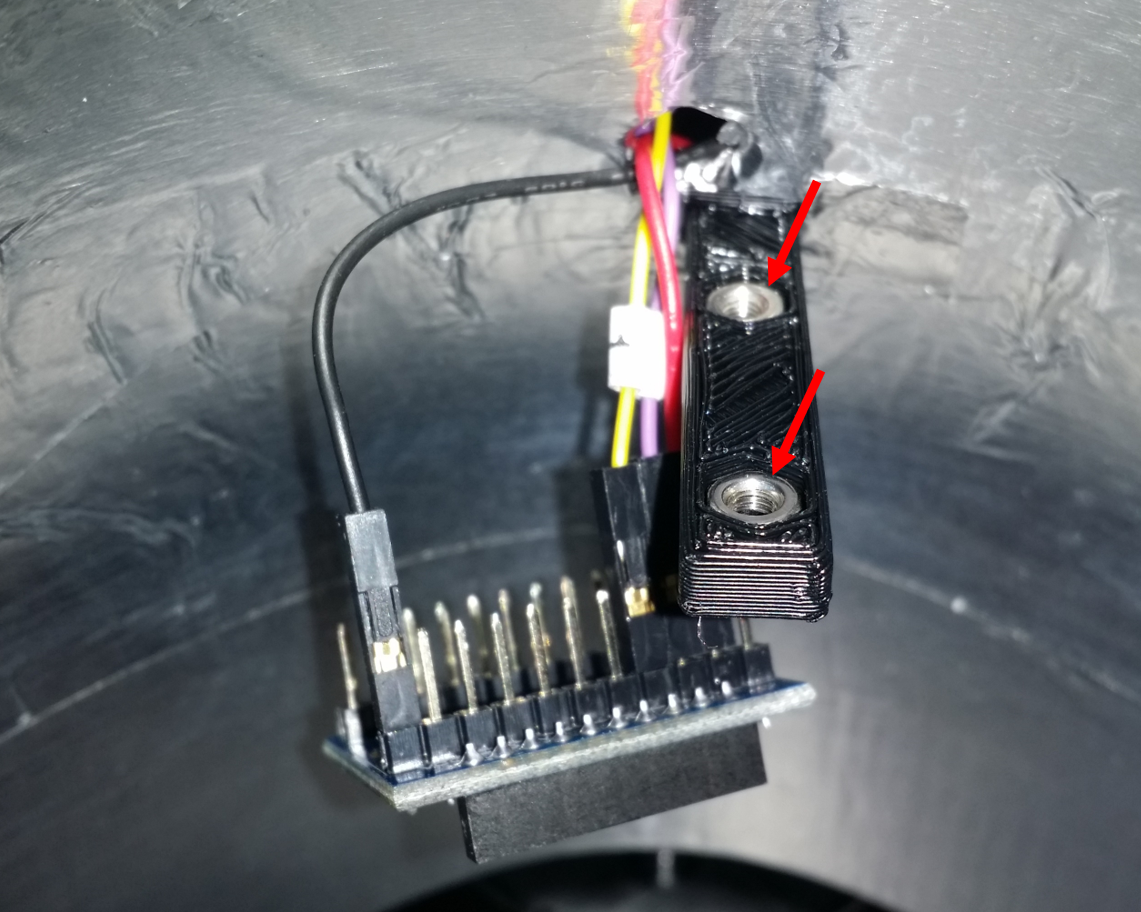
\includegraphics[width=4.2in]{figs/img/assembly/20-sideXBeeNuts.png}
        \caption{Nuts for Side XBee}
        \label{fig:sideXBeeNuts}
    \end{figure}

    \item Mount the XBee adapter board using two 8mm M3 screws (Fig. \ref{fig:sideXBeeMounting}). Make sure the board is oriented such that the antenna of the XBee will be toward the reflective surface.
    \begin{figure}[H]
        \centering
        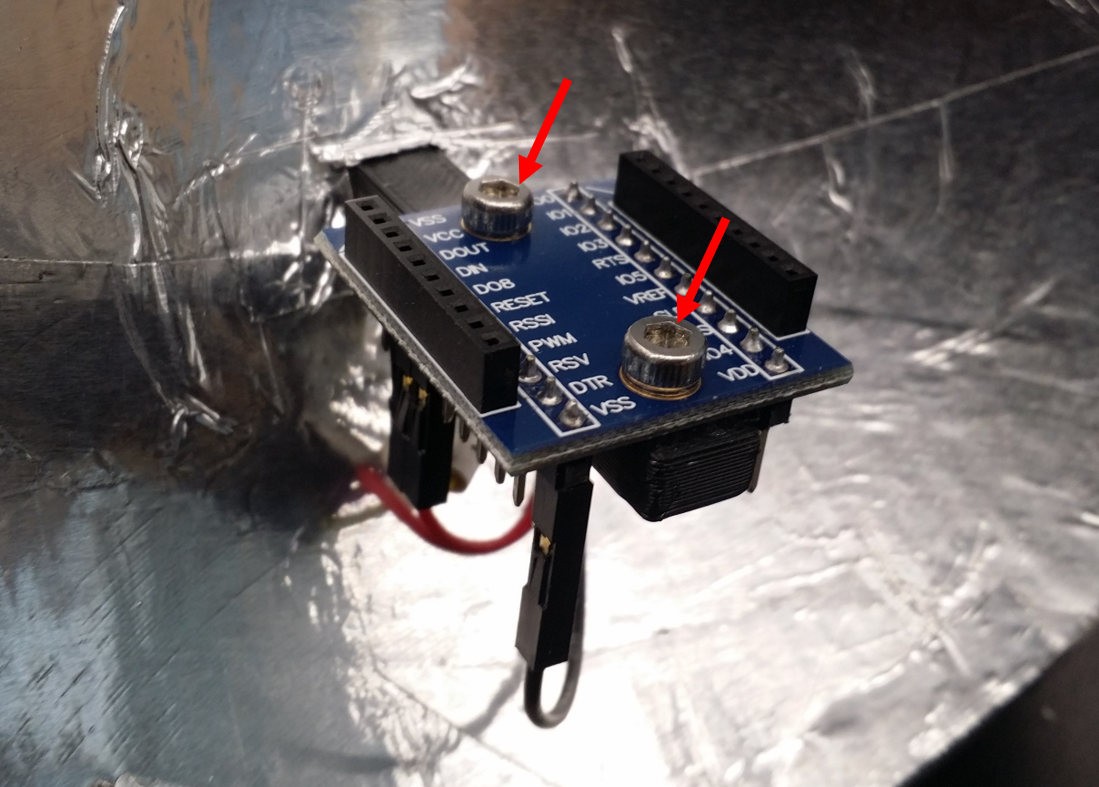
\includegraphics[width=4.2in]{figs/img/assembly/21-sideXBeeMounting.png}
        \caption{Mounting a Side XBee}
        \label{fig:sideXBeeMounting}
    \end{figure}
    \pagebreak

    \item Repeat steps 19 through 21 to mount XBee adapter boards into each of the four reflectors (Fig. \ref{fig:finishedSideXBees}).
    \begin{figure}[H]
        \centering
        \includegraphics[width=3.9in]{figs/img/assembly/22-finishedSideXBees.jpg}
        \caption{All Side XBees Mounted}
        \label{fig:finishedSideXBees}
    \end{figure}

    \item Wrap the wires coming from the reflector to keep them bundled into a single cable. Terminate the ends such that there is a 2-pin connector for +3.3V and GND (Fig. \ref{fig:reflectorWires}, red arrow), a 2-pin connector for the TX and RX to the top XBee (Fig. \ref{fig:reflectorWires}, blue arrow), a 4-pin connector for the TX pins of all four side XBees (Fig. \ref{fig:reflectorWires}, purple arrow), and a 4-pin connector for the RX pins of all four side XBees (Fig. \ref{fig:reflectorWires}, yellow arrow). Once again, it is useful to number both ends of the TX and RX wires to the side XBees.
    \begin{figure}[H]
        \centering
        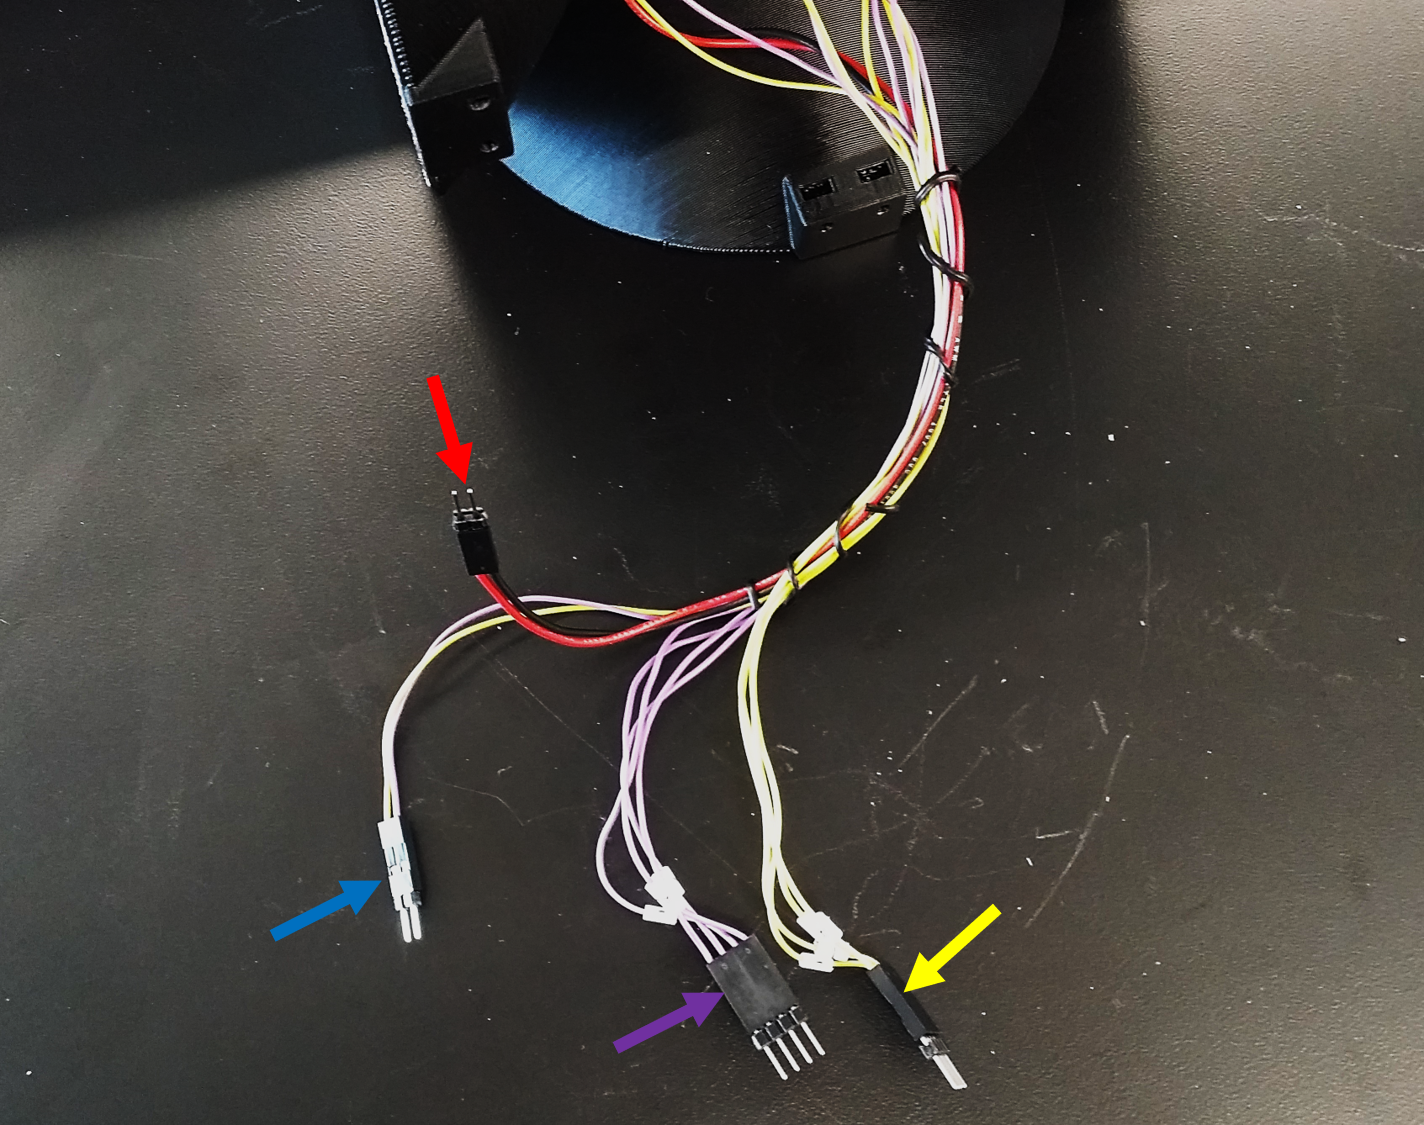
\includegraphics[width=3.9in]{figs/img/assembly/23-reflectorWireEnds.png}
        \caption{Reflector Wire Ends}
        \label{fig:reflectorWires}
    \end{figure}
    \pagebreak

    \item Insert two M3 nuts into the slots at the bottom of a reflector (Fig. \ref{fig:bottomNuts}). The nuts should recess into a hexagonal slot that prevents them from rotating.
    \begin{figure}[H]
        \centering
        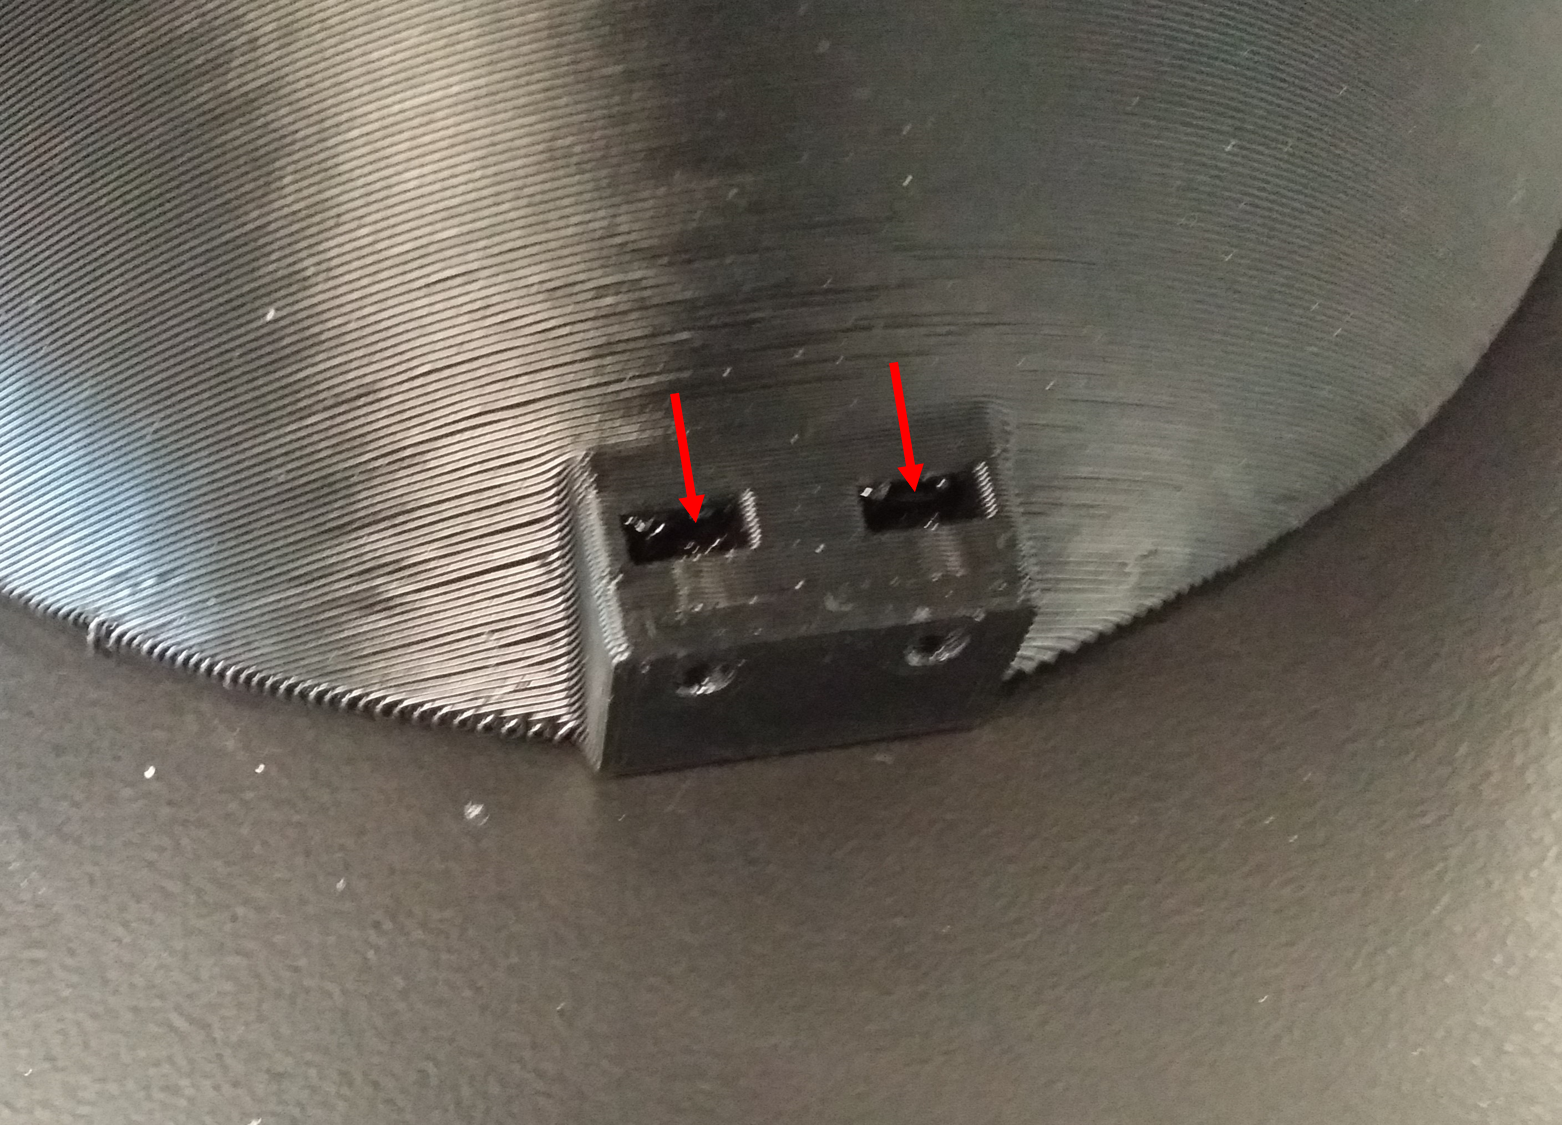
\includegraphics[width=3.6in]{figs/img/assembly/24-reflectorBottomNuts.png}
        \caption{Nuts for Bottom Frame}
        \label{fig:bottomNuts}
    \end{figure}

    \item Place the bottom frame onto the reflectors, with the stop plate pointed upward toward reflector 3. Route the wires through the hole between reflectors 1 and 2 (Fig. \ref{fig:reflectorWireRouting}).
    \begin{figure}[H]
        \centering
        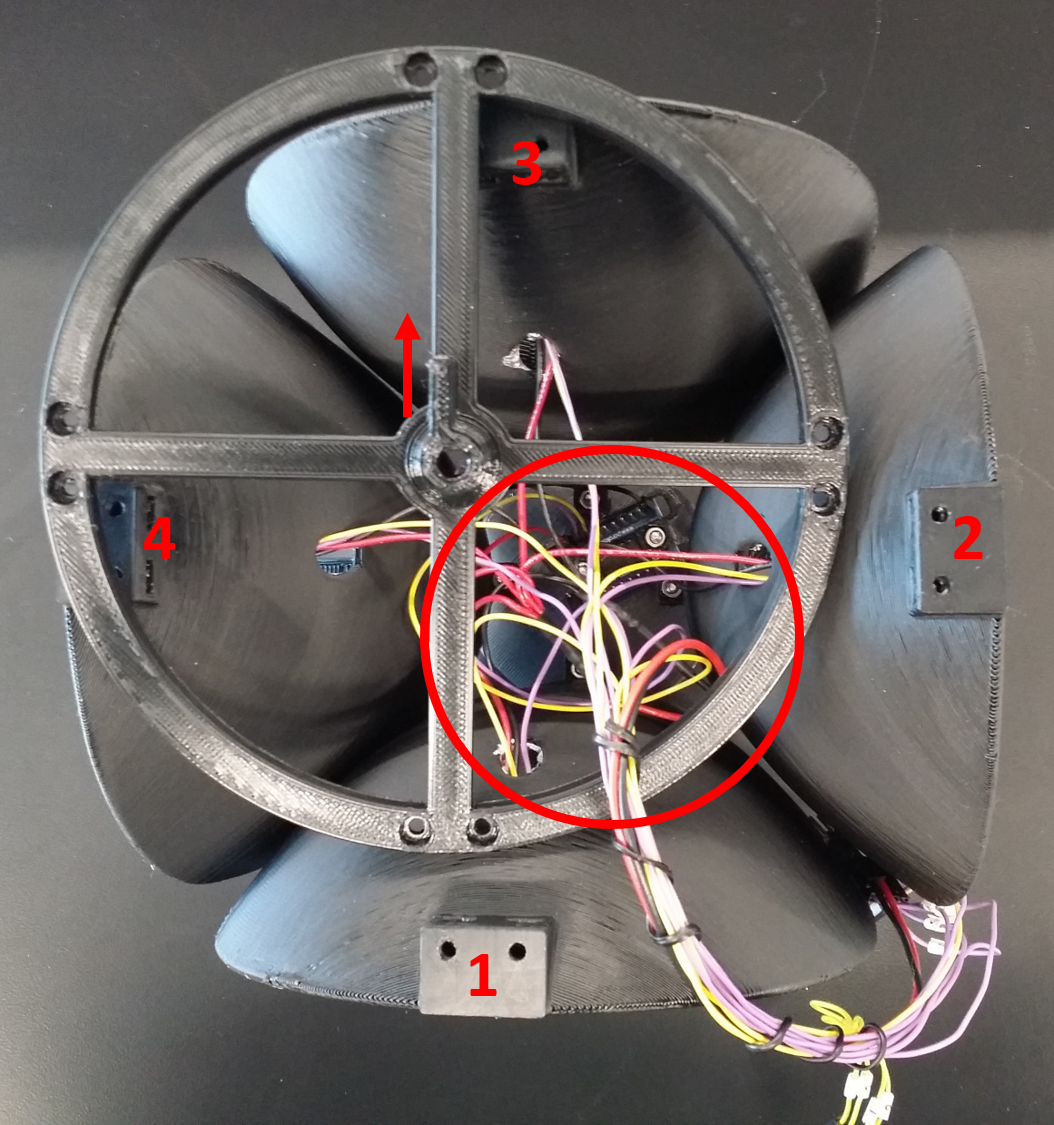
\includegraphics[width=3.9in]{figs/img/assembly/25-reflectorWireRouting.png}
        \caption{Reflector Wire Routing}
        \label{fig:reflectorWireRouting}
    \end{figure}
    \pagebreak

    \item Attach the bottom plate to the reflectors using eight 10mm M3 screws (Fig. \ref{fig:bottomMounting}).
    \begin{figure}[H]
        \centering
        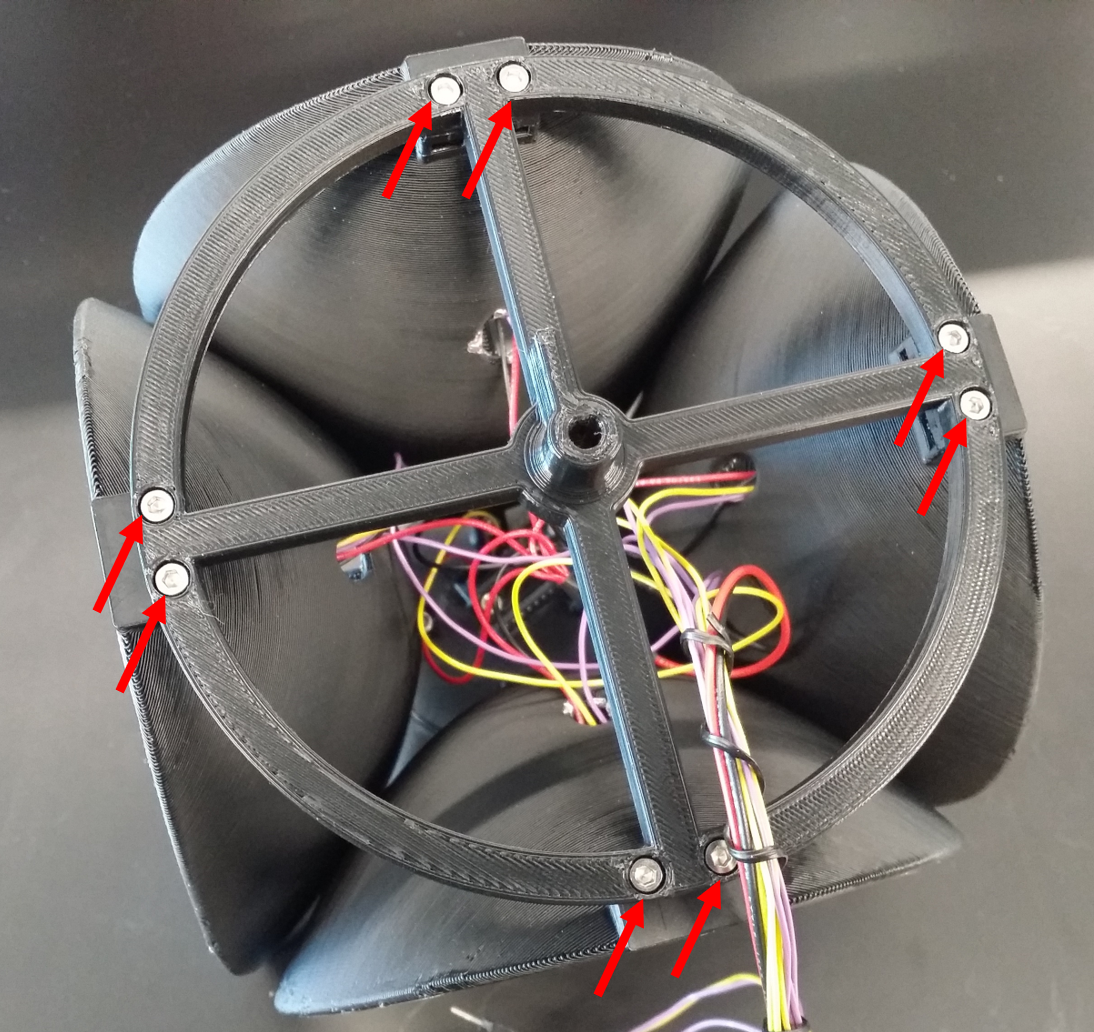
\includegraphics[width=3.6in]{figs/img/assembly/26-reflectorBottomMounting.png}
        \caption{Mounting the Bottom Frame}
        \label{fig:bottomMounting}
    \end{figure}

    \item Insert an XBee into each of the 5 XBee adapter boards (one on top and one in each reflector). Again, make sure that the XBees inside the reflectors are oriented with the antenna on the side toward the reflective surface (Fig. \ref{fig:XBeeInstallation}).
    \begin{figure}[H]
        \centering
        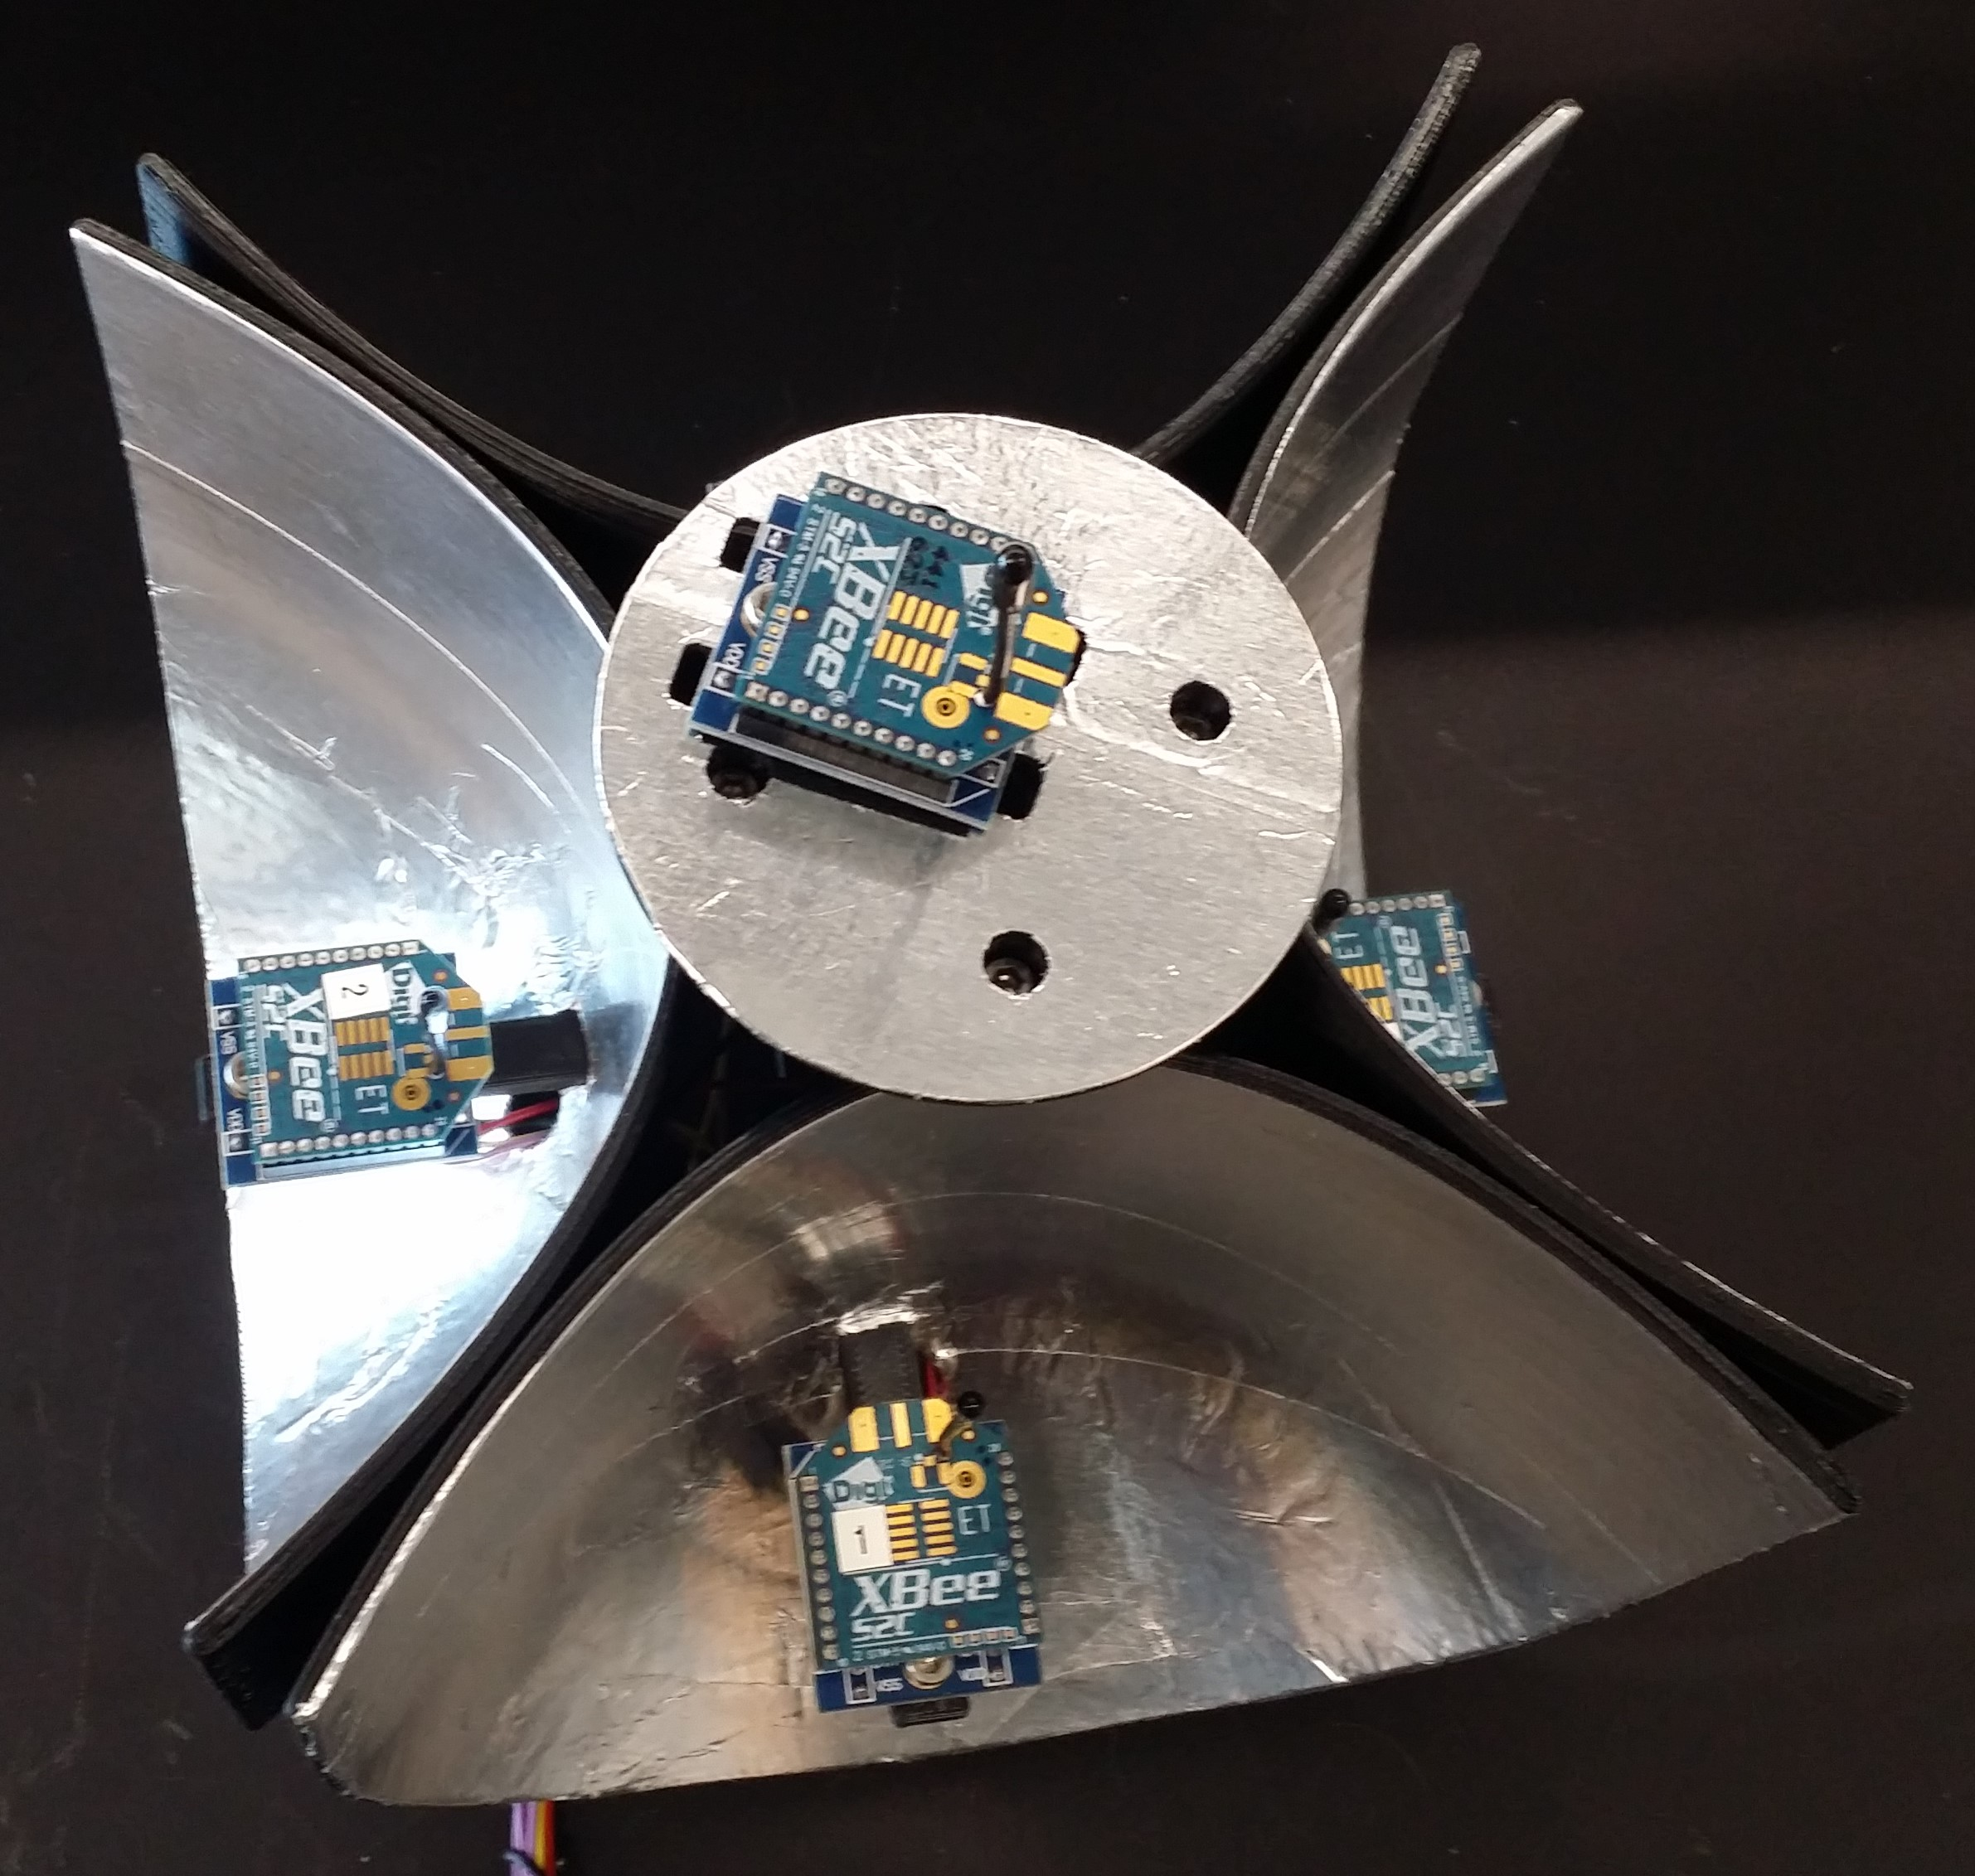
\includegraphics[width=3.6in]{figs/img/assembly/27-XBeeInstallation.jpg}
        \caption{XBee Installation}
        \label{fig:XBeeInstallation}
    \end{figure}
    \pagebreak

    \item Make sure the flat side of the stepper motor shaft is toward the back of the robot. Slide the reflector array onto this motor shaft, making sure the stop plate is pointed toward the back of the robot and is between the two stops on the stepper motor bracket (Fig. \ref{fig:reflectorMounting}).
    \begin{figure}[H]
        \centering
        \includegraphics[width=3.8in]{figs/img/assembly/28-reflectorMounting.png}
        \caption{Mounting the Reflectors on the Stepper Motor}
        \label{fig:reflectorMounting}
    \end{figure}

    \item Verify that the stop plate on the reflector array is between the stops on the stepper motor bracket (Fig. \ref{fig:installedReflector})
    \begin{figure}[H]
        \centering
        \includegraphics[width=3.8in]{figs/img/assembly/29-installedReflector.png}
        \caption{Reflector Stop Verification}
        \label{fig:installedReflector}
    \end{figure}
    \pagebreak

    \item Connect the reflector to the rest of the system by connecting the power cables to the output of the LM1117 regulator (Fig. \ref{fig:reflectorWiring}, red arrow), the top XBee TX and RX to the UART5 TX and RX (Fig. \ref{fig:reflectorWiring}, blue arrow), the side XBee TX wires to multiplexer pins 10 - 13 (Fig. \ref{fig:reflectorWiring}, purple arrow), and the side XBee RX wires to multiplexer pins 4 - 7 (Fig. \ref{fig:reflectorWiring}, yellow arrow). The side XBees should be connected to the multiplexer in order, with XBee 1 connecting to multiplexer pins 4 and 13.
    \begin{figure}[H]
        \centering
        \includegraphics[width=3.4in]{figs/img/assembly/30-reflectorWiring.png}
        \caption{Reflector Wiring}
        \label{fig:reflectorWiring}
    \end{figure}
\end{enumerate}

The robot assembly is complete! The fully assembled robot should look like the one shown in Fig. \ref{fig:assembledRobot}.
\begin{figure}[H]
    \centering
    \includegraphics[width=3.4in]{figs/img/assembly/31-assembledRobot.jpg}
    \caption{Assembled Robot}
    \label{fig:assembledRobot}
\end{figure}

%%% Local Variables:
%%% mode: latex
%%% TeX-master: "../finalReport"
%%% End:


% %----------------------------------------------------------------------
% % END MATERIAL
% %----------------------------------------------------------------------

% % B I B L I O G R A P H Y
% % -----------------------
% %
% % The following statement selects the style to use for references.  It controls the sort order of the entries in the bibliography and also the formatting for the in-text labels.
% \bibliographystyle{plain}
% % This specifies the location of the file containing the bibliographic information.  
% % It assumes you're using BibTeX (if not, why not?).
% \ifthenelse{\boolean{PrintVersion}}{
% \cleardoublepage % This is needed if the book class is used, to place the anchor in the correct page,
%                  % because the bibliography will start on its own page.
% }{
% \clearpage       % Use \clearpage instead if the document class uses the "oneside" argument
% }
% \phantomsection  % With hyperref package, enables hyperlinking from the table of contents to bibliography             
% % The following statement causes the title "References" to be used for the bibliography section:
% % \renewcommand*{\bibname}{References}
% Bibliography 
\renewcommand{\bibname}{Bibliography}

% Add the References to the Table of Contents
\addcontentsline{toc}{chapter}{\textbf{References}}

\bibliographystyle{IEEEtran}
\bibliography{bib/references.bib}
% Tip 5: You can create multiple .bib files to organize your references. 
% Just list them all in the \bibliogaphy command, separated by commas (no spaces).


%----------------------------------------------------------------------
\end{document}
%======================================================================



%%% Local Variables: 
%%% mode: latex
%%% TeX-master: t
%%% End: 
